%%%%%%%% ICML 2025 EXAMPLE LATEX SUBMISSION FILE %%%%%%%%%%%%%%%%%

\documentclass{article}

% Recommended, but optional, packages for figures and better typesetting:
\usepackage{microtype}
\usepackage{graphicx}
\usepackage{subcaption}
\usepackage{booktabs} % for professional tables

% hyperref makes hyperlinks in the resulting PDF.
% If your build breaks (sometimes temporarily if a hyperlink spans a page)
% please comment out the following usepackage line and replace
% \usepackage{icml2025} with \usepackage[nohyperref]{icml2025} above.
\usepackage{hyperref}


% Attempt to make hyperref and algorithmic work together better:
\newcommand{\theHalgorithm}{\arabic{algorithm}}

% Use the following line for the initial blind version submitted for review:
\usepackage{icml2025}

% If accepted, instead use the following line for the camera-ready submission:
% \usepackage[accepted]{icml2025}

% For theorems and such
\usepackage{amsmath}
\usepackage{amssymb}
\usepackage{mathtools}
\usepackage{amsthm}

% if you use cleveref..
\usepackage[capitalize,noabbrev]{cleveref}

%%%%%%%%%%%%%%%%%%%%%%%%%%%%%%%%
% THEOREMS
%%%%%%%%%%%%%%%%%%%%%%%%%%%%%%%%
\theoremstyle{plain}
\newtheorem{theorem}{Theorem}[section]
\newtheorem{proposition}[theorem]{Proposition}
\newtheorem{lemma}[theorem]{Lemma}
\newtheorem{corollary}[theorem]{Corollary}
\theoremstyle{definition}
\newtheorem{definition}[theorem]{Definition}
\newtheorem{assumption}[theorem]{Assumption}
\theoremstyle{remark}
\newtheorem{remark}[theorem]{Remark}

% Todonotes is useful during development; simply uncomment the next line
%    and comment out the line below the next line to turn off comments
%\usepackage[disable,textsize=tiny]{todonotes}
\usepackage[textsize=tiny]{todonotes}


% The \icmltitle you define below is probably too long as a header.
% Therefore, a short form for the running title is supplied here:
\icmltitlerunning{Submission and Formatting Instructions for ICML 2025}

\begin{document}

\twocolumn[
\icmltitle{Submission and Formatting Instructions for \\
           International Conference on Machine Learning (ICML 2025)}

% It is OKAY to include author information, even for blind
% submissions: the style file will automatically remove it for you
% unless you've provided the [accepted] option to the icml2025
% package.

% List of affiliations: The first argument should be a (short)
% identifier you will use later to specify author affiliations
% Academic affiliations should list Department, University, City, Region, Country
% Industry affiliations should list Company, City, Region, Country

% You can specify symbols, otherwise they are numbered in order.
% Ideally, you should not use this facility. Affiliations will be numbered
% in order of appearance and this is the preferred way.
\icmlsetsymbol{equal}{*}

\begin{icmlauthorlist}
\icmlauthor{Firstname1 Lastname1}{equal,yyy}
\icmlauthor{Firstname2 Lastname2}{equal,yyy,comp}
\icmlauthor{Firstname3 Lastname3}{comp}
\icmlauthor{Firstname4 Lastname4}{sch}
\icmlauthor{Firstname5 Lastname5}{yyy}
\icmlauthor{Firstname6 Lastname6}{sch,yyy,comp}
\icmlauthor{Firstname7 Lastname7}{comp}
%\icmlauthor{}{sch}
\icmlauthor{Firstname8 Lastname8}{sch}
\icmlauthor{Firstname8 Lastname8}{yyy,comp}
%\icmlauthor{}{sch}
%\icmlauthor{}{sch}
\end{icmlauthorlist}

\icmlaffiliation{yyy}{Department of XXX, University of YYY, Location, Country}
\icmlaffiliation{comp}{Company Name, Location, Country}
\icmlaffiliation{sch}{School of ZZZ, Institute of WWW, Location, Country}

\icmlcorrespondingauthor{Firstname1 Lastname1}{first1.last1@xxx.edu}
\icmlcorrespondingauthor{Firstname2 Lastname2}{first2.last2@www.uk}

% You may provide any keywords that you
% find helpful for describing your paper; these are used to populate
% the "keywords" metadata in the PDF but will not be shown in the document
\icmlkeywords{Machine Learning, ICML}

\vskip 0.3in
]

% this must go after the closing bracket ] following \twocolumn[ ...

% This command actually creates the footnote in the first column
% listing the affiliations and the copyright notice.
% The command takes one argument, which is text to display at the start of the footnote.
% The \icmlEqualContribution command is standard text for equal contribution.
% Remove it (just {}) if you do not need this facility.

%\printAffiliationsAndNotice{}  % leave blank if no need to mention equal contribution
\printAffiliationsAndNotice{\icmlEqualContribution} % otherwise use the standard text.

\begin{abstract}
This document provides a basic paper template and submission guidelines.
Abstracts must be a single paragraph, ideally between 4--6 sentences long.
Gross violations will trigger corrections at the camera-ready phase.
\end{abstract}


\section{Introduction}
\label{Introduction}
With the development of Internet of Things(IoT), many end devices are generating plenty of data each day.
Due to the growing storage and computing power, it becomes more appealing to store data locally and push more compution function to them.
It motivates the application of federated learning, which supports local storage and local training on each device without violating their privacy.

As shown in Fig.1, a federated learning system comprises a central server and a large number of clients(i.e. end devices).
The central server maintains a global model while each client owns local statistic.
During each iteration, the clients download global model from the central server and makes local updates on their private data. Then the central server will aggregate the updated models from the clients and generate a new global model.
The training process will terminate when the accuracy of global model has reached the preset threshold.
During the process, since the clients share not their private data but the trained local model with the central server, the federated learning system can protect clients' privacy efficiently.

Despite its advantage in enabling collaborating learning while protecting data privacy, it still faces some key challenges.
The first challenge is design of incentive mechanism.
In FL model training, the clients usually consume massive amount of resources, including computing capacity, communication bandwidth and battery charge.
Considering excessive resources expenditure, clients would be reluctant to participate in FL model training without sufficient economic compensation.
Therefore, the central server needs to encourage clients to contribute their data and resources for the FL model training by offering sufficient payment. 
There are plenty of works focusing on the design of incentive mechanism in FL, varing from game theory [1], [2] to contract theory [3] and acution theory[4].
However, these works don't consider the scenarios of dynamic data stream. In reality, these clients(or end devices) can generate new data continuously.
In this case, design of incentive mechanism for scenarios where clients own static local data can not be applied directly in scenarios where clients with dynamic data stream.

The second challenge is the uncertainty caused by dynamic data stream. 
In reality, clients may generate new data continuously. 
For example, a smartphone owner may take pictures or send messages at any time. These new data are then stored in its internal storage.
When participating in FL model training, continuously generated new data will arrive in real time and cause severe data shift and training uncertainty [4] compared with scenarios where clients own pre-determined static dataset.
There are a few works studying the FL method in the scenarios with dynamic data stream. [4][5] try to manage data stream by introducing a medium buffer in order to reduce the negative impact of data uncertainty on training process. [6][7] provide the convergence guarantee in FL with dynamic data stream and model a new federated optimization problem.
However, these works don't analyse the behaviour of central server and clients from a perspective of economy. That is, they don't take model clients and central server's reward and expenditure into account.

Motivated by the above discussions, in this article, we propose a new federated learning framework, FedStream. This framework is a kind of incentive mechanism for FL with dynamic data stream.  
Specially, before each iteration, the central server first announce its FL task and total payment, then the clients choose its optimal amount of data generation.

\section{Related Work}
\label{Related Work}
\subsection{Federated Learning on Incentive Mechanism}
Incentive mechanism designed for federated learning has been widely studied in previous works.
They can be assorted into three catagories:
(1) \textbf{game theory:} [10]  proposes a hierarchical incentive mechanism based on coalitional game theory approach, where multiple workers can form various federations.
[11] designs a novel incentive framework based on Stackelberg game to model the collaboration behaviour among server and clients in federated learning with difference privacy.
[12] builds a incentive mechanism utilizing repeated game theory to enable long-term cooperation among participants in cross-silo federated learning.
(2) \textbf{auction theory:} [13] adopts auction theory for wireless federated learning services market and builds a reverse auction mechanism to maximize the social welfare.
(3) \textbf{contract theory:} [14] introduces a contract theory based incentive mechanism to stimulate workers to update data, which can balance the trade off between age of information and service latency.
[15] presents an incentive mechanism leveraging contract theory to encourage workers with high reputation and high data quality to take part in federated learning tasks.

In addition, there are some other methods to be utilized for design of incentive mechanism in federated learning.
[16] designs an incentive mechanism based on deep reinforcement learning, in which the central server can adjust the optimal price strategy dynamically in accordance with the uncertain environment.
[17] proposes a blockchain based incentive mechanism in hierarchical federated learning for end-edge-cloud communications, which prevents unreliable participants' disturbance and further ensure data privacy efficiently.

However, the above studies only consider the scenario that each client owns a static dataset. They ignore the fact that clients can generate new data continuously.
Thus, the incentive mechanism designed on the basis of static dataset cannot be applied to federated learning tasks against dynamic data stream directly.

\subsection{Learning upon Streaming Data}
Machine learning on streaming data faces key challenges including uncertain arrival patterns, limited storage and so on.
To deal with the challenges, [18] proposes an online learning algorithm of strSAGA, which maintains a buffer between arrived data and training data to handle the uncertainty of data arrival patterns.
In addition, to enhance the stability of convergence, the gradient used for model updating is computed on new data points at first and then revised by previous data points.
However, this work doesn't extend strSAGA to distributed machine learning.

The study in [19] introduces strSAGA into federated learning, which considers the features of streaming data and convergence of federated learninig at the same time.
[20] jointly optimizes the number of local update and mini batch size to strike the trade off among accuracy, expenditure and time latency in federated learning with streaming data.
[30] combines federated learning with online data management and computation offloading, trying to find the best model aggregation frequency and data offloading rate to promote model performance and reduce cost expenditure.
However, all the above works neglect the expenditure and utility in the clients' side while training, which may leads to clients' reluctance to participate in federated learning task.

\section{Preliminary Knowledge}
\subsection{Federated Learning with Data Stream}
\begin{figure}[ht]
  \centering
  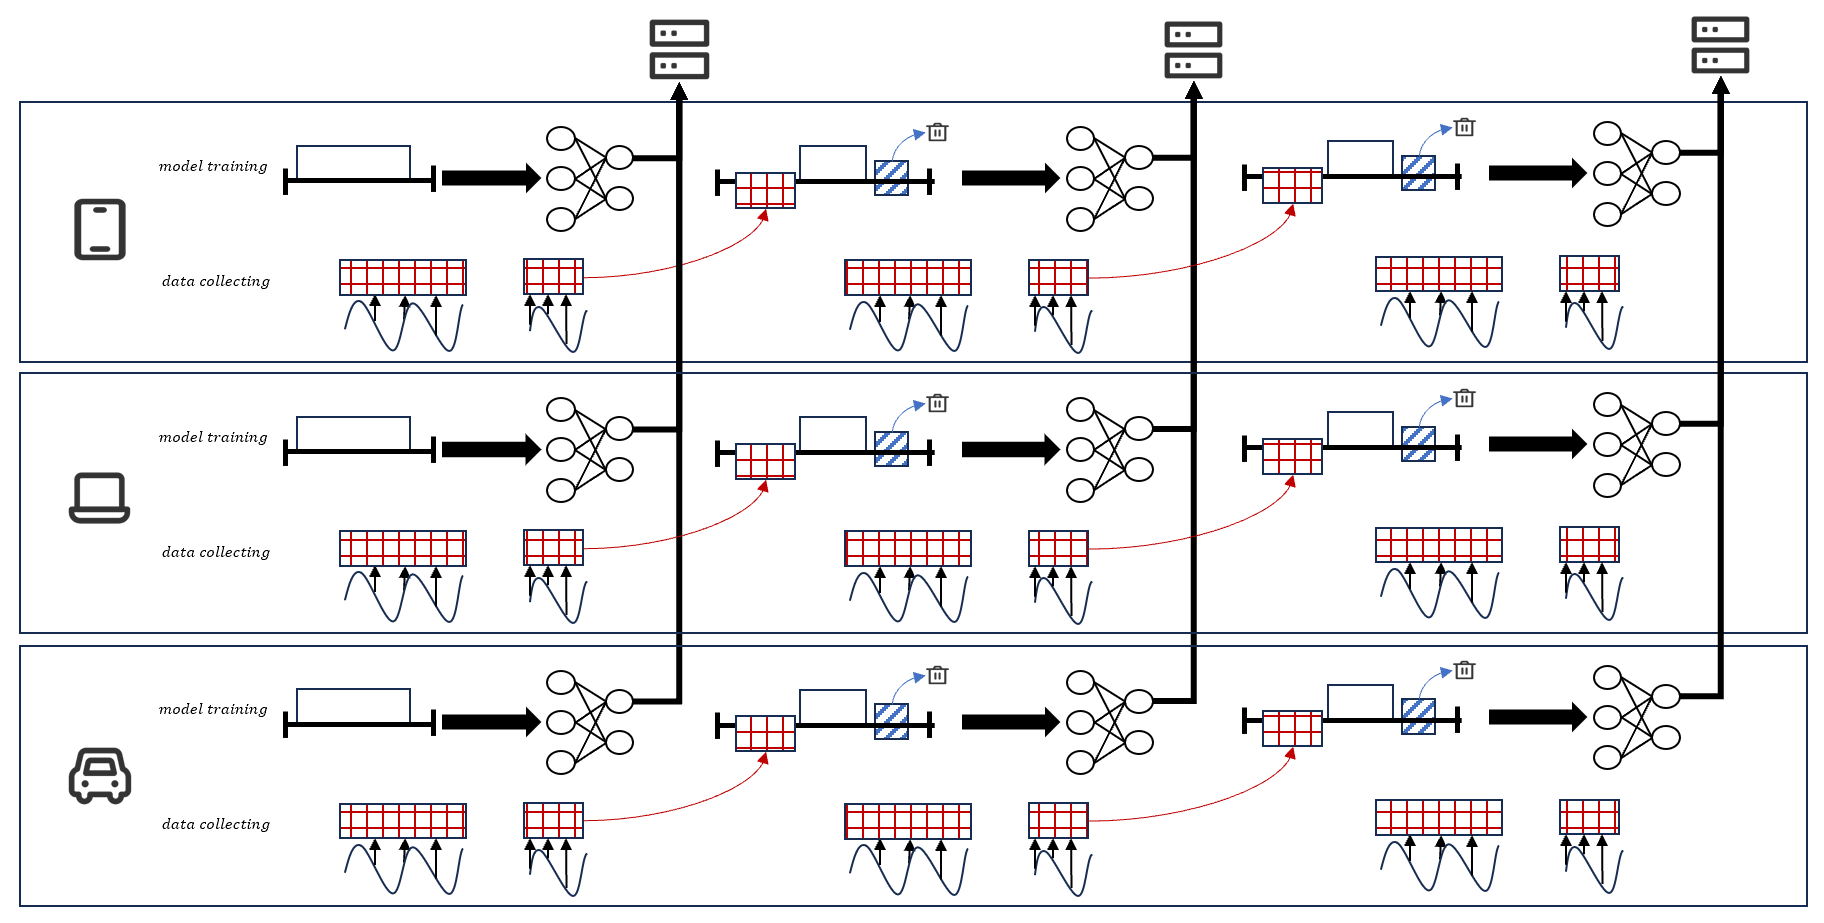
\includegraphics[width=\columnwidth]{figures/figure_21.png}
  \caption{Framework}
\end{figure}
We assume that there is a central server and $N$ clients in the federated learning system and they are arranged to conduct $T$ rounds in the training task. Different from the static local dataset in previous works, each client $k$ has a local data stream $\mathcal{D}_k$ which generates new data points randomly and dynamically over the time horizen.
In addition, due to the storage limit, each client maintains a buffer to store data points sampled from its data stream $\mathcal{D}_k$ and used for FL model training.
We denote the stored data points in the buffer of client $k$ at round $t$ as $\mathcal{D}_k(t)$ and $\vert\mathcal{D}_k(t)\vert = D_k(t)$. 
During each round, the buffer of client $k$ can be updated by decaying part of stale data points and sampling new ones from its local data stream, and then used for local model training.
Therefore, the updating strategy of client $k$ at round $t$ can be modeled as
\begin{equation}
  D_k(t+1) = \theta D_k(t) + \Delta_k(t),
\end{equation}
where $\theta \in [0,1]$ is the conservation rate of stale data points and it effects the degree of staleness. 
Besides, $\Delta_k(t)$ is the amount of newly collected data points during round $t$.

Note that considering the uncertainty of data stream, data collection cannot be completed immediately, which means the traditional "collecting-training" paradigm may lead to severe time latency for federated learning task.
To improve the task efficiency, data collection is designed to proceed in parallel with model training in our framework, and the newly collected data points during this round will be used to update buffer and train model for the next round, as depicted in Fig 1.

Then, the loss function of client $k$ based on global model $w(t)$ using stored data points $\mathcal{D}_k(t)$ at round $t$ can be represented as 
\begin{equation}
  F_k(w(t), \mathcal{D}_k(t)) = \frac{1}{D_k(t)} \sum_{j=1}^{D_k(t)} f(w(t), x_k^j),
\end{equation}
where $f(w(t), x_k^j)$ is the loss function of each data point $\{x_k^j, y_k^j\} \in \mathcal{D}_k(t)$.
Then client $k$ updates its local model and injects noise as
\begin{equation}
  w_k(t+1) = w(t) - \eta \nabla F_k(w(t), \mathcal{D}_k(t)),
\end{equation}
where $\eta$ is the learning rate and $\nabla F_k(w(t), \mathcal{D}_k(t))$ is the loss gradient of client $k$ at round $t$. 
Until each client completes its local update and sends $w_k(t+1)$ to the central server, the central server will aggregate them by
\begin{equation}
  w(t+1) = \sum_{k=1}^{N} \frac{D_k(t)}{D(t)} w_k(t+1),
\end{equation}
where $\mathcal{D}(t) = \cup_{k=1}^N \mathcal{D}_k(t)$ and $D(t) = \sum_{k=1}^{N} D_k(t)$.
Subsequently, the central server launches the new global model $w(t+1)$ to each client for the next round's training.
The global loss function at round $t$ can be represented as
\begin{equation}
  F(w(t), \mathcal{D}(t)) = \sum_{k=1}^{N} \frac{D_k(t)}{D(t)} F_k(w(t), \mathcal{D}_k(t)).
\end{equation}
The ultimate goal is to find optimal parameters $w(t), t \in [0, \cdots, T-1]$ to minimize the global loss function in each round $t$, which can be expressed as
\begin{equation}
  \arg \min_{w(t)} F(w(t), \mathcal{D}(t)) = \sum_{k=1}^{N} \frac{D_k(t)}{D(t)} F_k(w_k(t), \mathcal{D}_k(t)).
\end{equation}

\subsection{Convergence Analysis for Federated Learning with Data Stream}
Model performance convergence analysis for FedStream is provided in this section.
In practice, it's difficult to measure the model performance of FedStream directly due to data dynamity, data heterogeneity and so on.
To overcome the challenge, previous works have leveraged the convergence bound of the expected difference between the training loss and the optimal loss to capture the model performance.
In this section, we adopt this method and provide a convergence upperbound for federated learning with data stream, considering the impact of data quantity, data heterogeneity and data staleness on final model performance.
Before that, the concept of degree of staleness(DoS) for data points is introduced in Definition 1.
\begin{definition}
  We denote $S_k(t)$ as the degree of staleness(DoS) for client $k$'s data samples at round $t$. In FedStream, the recursive definition is provided as 
  \begin{equation}
    S_k(t) = 
    \begin{cases}
      \dfrac{\theta D_k(t-1)}{D_k(t)}(S_k(t-1) + 1) + \dfrac{\Delta_k(t-1)}{D_k(t)}, & t > 0; \\
      1, & t = 0,
    \end{cases}
  \end{equation}
  where $S_k(t)$ is the weighted sum of previous data points' DoS and the new data points' DoS.
  The previous data points' DoS should be updated by adding to $1$ when stepping into the next time slot. And the new data points' DoS is set to be $1$.
\end{definition}

Then, we have the following properties:
\begin{corollary}
  $S_k(t)$ increases with conservation rate $\theta$ and decreases with increment $\Delta_k(t)$, which reflects the fact that less stale data samples and more fresh ones brings the reduction of DoS.
\end{corollary}

\begin{corollary}
  The general formula of $S_k(t)$ can be further provided as
  \begin{equation}
    S_k(t) = \sum_{\tau=0}^{t} \frac{\theta^{t-\tau} D_k(\tau)}{D_k(t)}.    
  \end{equation}
\end{corollary}

\begin{assumption}
  $F_k(w)$ is $\rho$-Lipschitz, i.e., $F_k(w) - F_k(w^{'}) \leq \rho \Vert w - w^{'} \Vert_2$.
\end{assumption}
\begin{assumption}
  $F_k(w)$ is $\beta$-Lipschitz smooth, i.e., $\Vert\nabla F_k(w) - \nabla F_k(w^{'})\Vert \leq \beta \Vert w-w^{'} \Vert_2$.
\end{assumption}
\begin{assumption}
  $F_k(w)$ is $\mu$-strong contex, i.e., $F_k(w)$ satisfies $F_k(w) - F_k(w^*) \leq \frac{1}{2\mu}\Vert\nabla F_k(w)\Vert_2^2$.
\end{assumption}
\begin{assumption}
  The stochastic gradient is unbiased and variance-bound, that is, $E[\nabla F_k(w(t)|D_k(t))] = \nabla F_k(w(t)|\mathcal{D}_k)$ and $E\Vert\nabla F_k(w(t)|D_k(t)) - \nabla F_k(w(t)|\mathcal{D}_k)\Vert^2 \leq \frac{\psi^2}{D_k(t)}$. 
\end{assumption}
\begin{assumption}
  The data heterogeneity is bounded, i.e, $\Vert \nabla F_k(w(t)|\mathcal{D}_k) - \nabla F(w(t)|D(t)\Vert \leq \delta_{k,t}$. 
\end{assumption}
\begin{assumption}
  The expected square norm of stochastic gradient is bounded, i.e., $E\Vert \nabla F_k(w(t)|D_k(t))\Vert^2 \leq G_k^2 + S_k(t)\sigma^2$, where $\sigma$ is the sensitivity coefficient of client $k$ to the freshness of data samples.
\end{assumption}

\begin{theorem}
  Under Assumptions 1-6, with $\eta \leq \frac{1}{2\beta}$, $\xi \geq 2$, the convergence upperbound after $T$ rounds can be formulated as
  \begin{align}
      & E[F(w(T)|D(T)) - F(w^*)] \notag \\ 
 \leq & \underbrace{\vphantom{\sum_{min}^{max}\frac{1}{2}} \kappa_1^{T} E[F(w(0)|D(0))-F(w^*)]}_{(1)} \notag \\
      & + \sum_{t=0}^{T-1} \kappa_1^{T-1-t} \left[\underbrace{\vphantom{\sum_{min}^{max}\frac{1}{2}} \kappa_2 \frac{N\psi^2}{D(t)}}_{(2)} + \underbrace{\vphantom{\sum_{min}^{max}\frac{1}{2}} \kappa_3 \sum_{k=1}^{N} \frac{D_k(t)}{D(t)} S_k(t) \sigma^2}_{(3)} + \underbrace{\vphantom{\sum_{min}^{max}\frac{1}{2}} \kappa_4 \sum_{k=1}^{N} \frac{D_k(t)}{D(t)} \overline{\delta_k}^2}_{(4)} + \underbrace{\vphantom{\sum_{min}^{max}\frac{1}{2}} \Omega_{t}}_{(5)}\right]. \notag \\ 
  \end{align}
  where $\Omega_t = F(w(t+1)|D(t+1)) - F(w(t+1)|D(t))$,
  and $\overline{\delta_k} \triangleq \max_{0 \leq t \leq T-1} \delta_{k,t}$ with $\delta_{k,t} = \Vert \nabla F_k(w(t)|\mathcal{D}_k) - F(w(t)|D(t)) \Vert$.
  In addition, $\kappa_1 = 1 + 4\mu\beta\eta^2 - 2\mu\eta$, $\kappa_2 = 2\beta\eta^2$, $\kappa_3 = \beta\eta^2$ and $\kappa_4 = 2\xi\beta\eta^2 + \frac{1}{2}\xi\eta$. 
\end{theorem}

The detailed proof is provided in Appendix A.1.
\begin{remark}
  In the fifth term of Theorem 1, $\Omega_t$ captures the expected difference of global loss function based on the same global model $w(t)$ between total stored data points at current round $\mathcal{D}(t)$ and at previous round $\mathcal{D}(t-1)$.
  Note that $\Omega_t$ is time-varying and it measures the influence of data dynamity has on model performance, and describes the generalization of global model towards new data points. 
  The more fluctuating data dynamity is, the larger the convergence bound is and the worse the global model performs. 
\end{remark}
\begin{remark}
  In the fourth term of Theorem 1, $\delta_{k,t}$ captures the gradient gap between the global loss function and the local loss function of client $k$ at the round $t$. 
  It measures the degree of data heterogeneity for client $k$ at round $t$. Note that due to data dynamity, $\delta_{k,t}$ is time-varying, too.
  Thus, we define $\overline{\delta_k}$ to represent the upperbound of $\delta_{k,t}$ across the time slots $t \in [0, T-1]$. The fourth term describes the impact of global data heterogeneity degree on model performance.
  According to this term, within single round $t$, the convergence bound would be reduced if a client with smaller $\overline{\delta_k}$ stores more data points for training than others.
\end{remark}

\section{System Model}
In this section, we design an incentive mechanism for federated learning with data stream, called FedStream.
This section starts with the workflow of FedStream in $4.1$. Then the cost function of central server and the utility function of clients will be demonstrated in $4.2$ and $4.3$ respectively.
Ultimately, we model this federated learning system interaction with a two-stage Stackelberg Game.
\subsection{Overview}
\begin{figure}[ht]
  \centering
  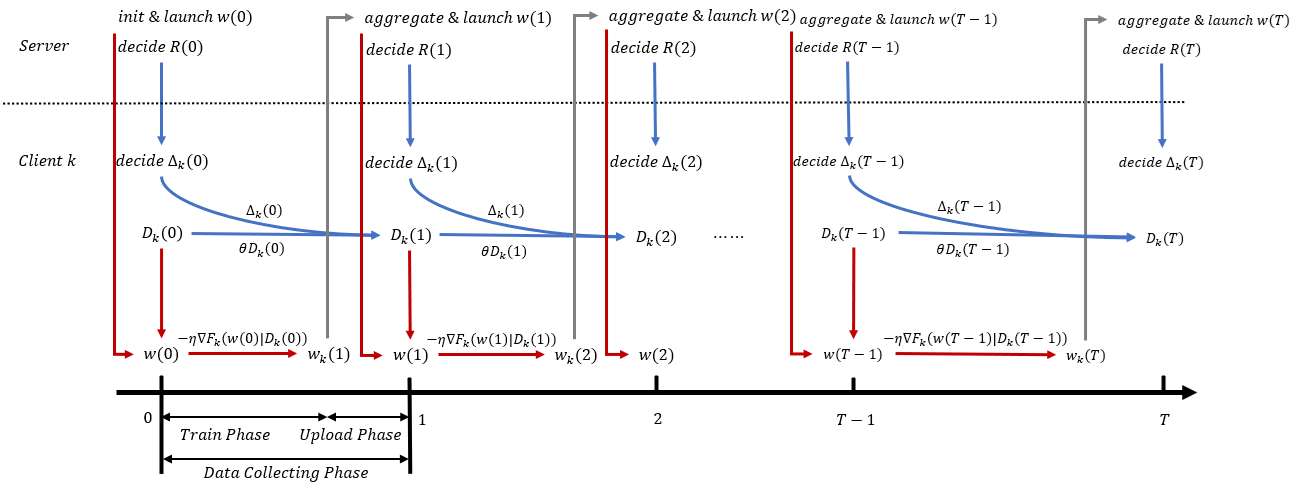
\includegraphics[width=\columnwidth]{figures/figure_17.png}
  \caption{Timeline}
\end{figure}
Assume that there is a central server and $N$ clients, each client holds a local data stream and a buffer with stored data points sampled from its local data stream. 
The central server needs to conduct $T$ rounds in its FL task. 
At each round $t$, the central server launches the global model $w(t)$ to all clients.
Considering clients may be reluctant to collect data and train model actively due to various expenditure, the central server also provides some payment $R$ to them.

After downloading global model from the central server, each client begins to train model $w(t)$ using data points stored in buffer, i.e. $\mathcal{D}_k(t)$. 
Moreover, stimulated by the payment $R$, clients attempt to sample some new data points from their local data stream.
The amount of newly sampled data points $\Delta_k(t)$ is determined by themselves based on the central server's payment $R$ and other clients' decisions.
It deserves to be noted repeatedly that model training and data sampling proceed in parallel and that the newly sampled data points are prepared for the next round's buffer updating and model training.

When all clients upload their local models to the central server, it aggregates their local model and obtains a new global model $w(t+1)$.
In round $t + 1$, the central server will launch new global model $w(t+1)$ and payment $R$. For each client $k$, it adds new data points sampled during last round, i.e., $\Delta_k(t)$ into buffer and generates $\mathcal{D}_k(t+1)$ at first, then they use $\mathcal{D}_k(t+1)$ to train $w(t+1)$. 
Meanwhile, they decide the amount of newly sampled data points $\Delta_k(t+1)$ and sample for round $t+2$. 

For ease of demonstration, we define $\boldsymbol{D_k} = \{D_k(0), D_k(1), \cdots, D_k(T-1)\}$ and it's the decision sequence of client $k$'s buffer size during the training period.
Furthermore, we define $\boldsymbol{D} = \{\boldsymbol{D_1}, \boldsymbol{D_2}, \cdots, \boldsymbol{D_N}\}$ as the composition of all clients' buffer size sequence throughout the training.
In our framework, both $R$ and $\boldsymbol{D}$ need to be pitched precisely.
In the next section, we will construct a rigorous model to unveil the behaviour of both the central server and all clients.
Then based on this model, we try to explore the optimal payment $R$ for central server and optimal buffer vector $\boldsymbol{D_k}$ for each client $k \in \mathcal{N}$.


\subsection{Cost Function of Central Server}
From the prespective of the central server, on the one hand, it needs to stimulate clients to participate in model training to achieve a better model performance.
On the other hand, it needs to control the payment to clients at the same time.
Hence, the expenditure of the central server comprises two parts: accuracy loss of model and payment to clients. 
In reality, it's extremely hard to obtain accurate form of model accuracy loss directly. Yet we can approximate it with the convergence upperbound provided in Theorem 1.
Note that $(1)$ and $(5)$ in Theorem 1 cannot be controlled by the central server, hence we extract the valid part of $(2)$, $(3)$ and $(4)$ to the cost function.
In addition, total payment during the training period offered to clients can be represented as $TR$.
Then, the cost function of the central server can be constructed as the sum of accuracy loss of model and total payment to clients as
\begin{equation}
  U(\boldsymbol{D}, R, \theta) = \sum_{t=0}^{T-1}\left[(1-\gamma)\kappa_1^{T-1-t} \left(\kappa_2 \frac{N\psi^2}{D(t)} + \kappa_3 \sum_{k=1}^{N} \frac{D_k(t)}{D(t)} S_k(t) \sigma^2 + \kappa_4 \sum_{k=1}^{N} \frac{D_k(t)}{D(t)} \overline{\delta_k}^2\right) + \gamma R\right],
\end{equation}
where $\gamma \in [0, 1]$ is a factor to strike the balance between model performance and cost payment. When $\gamma$ trends to $1$, the central server pays more attention to enhancing the model performance. Otherwise, the central server prefers to save cost payment.
By observing (10), the cost function of central server is dominated by $\boldsymbol{D}$ and $R$ simultaneously.
In the cost function, a greater payment $R$ encourages clients to sample more data points and maintains a greater buffer for the next round, which helps to reduce accuracy loss and enhance model performance. But the total payment to clients increase at the same time. There's a trade off in the cost function.
Hence, the optimization problem on the central server's side can be modeled as
\begin{equation}
  \min_{R,\theta}  U(\boldsymbol{D}, R, \theta), 
\end{equation}
where the central server's target is to minimize its cost function $U(\boldsymbol{D}, R, \theta)$ by navigating the optimal payment $R$ and decay factor $\theta$.

\subsection{Utility Function of Clients}
For a client who participates into the federated learning task, it needs to spend various types of resource for data sampling and model training.
Here, we use $\alpha_k \Delta_k(t)^2$ and $\beta_k D_k(t)^2$ to depict the expenditure for data collecting and training, respectively, where $\alpha_k$ is unit cost for data collecting and $\beta_k$ is the counterpart for model training.
It should be noted that we choose the quadratic form of $\Delta_k(t)^2$ and $D_k(t)^2$ to reflect the fact that a client's sampling and training expenditure should convexly increase with its increment and scale, respectively.
Therefore, the cost can be expressed as
\begin{equation}
  C_k(t) = \alpha_k \Delta_k(t)^2 + \beta_k D_k(t)^2.
\end{equation}

Meanwhile, a client can obtain some payment.
The payment received by a client is proportional to its contribution to model performance and inversely proportional to others' contribution.
In FedStream, a client's contribution should consider three aspects: privacy budget $\varepsilon_k$, buffer size $D_k(t)$ and data heterogeneity $\overline{\delta_k}$.
Specially, it is proportional to $D_k(t)$, as well as inversely proportional to $\overline{\delta_k}$.
Thus, the payment received by a client can be formulated as
\begin{equation}
  P_k(t) = \frac{\overline{\delta_k}^{-1}D_k(t)}{\sum_{i=1}^{N}\overline{\delta_i}^{-1}D_i(t)}R,
\end{equation}
where $\sum_{i=1}^{N} \overline{\delta_i}^{-1}D_i(t)$ can be considered as the total contribution of all clients make to model performance.
Then, the utility function of client $k$ is constructed as the sum of gap between payment and cost over the time horizen:
\begin{equation}
  U_k(\boldsymbol{D_k}, \boldsymbol{D_{-k}}, R, \theta) = \sum_{t=0}^{T-1} \left(P_k(t) - C_k(t)\right),
\end{equation}
where $\boldsymbol{D_{-k}} = \boldsymbol{D}$ \textbackslash $\boldsymbol{D_k}$ and it's the set of all clients' buffer size except for client $k$. 
The utility of client $k$ is dominated by its own buffer size vector $\boldsymbol{D_k}$, other clients' buffer size vector $\boldsymbol{D_{-k}}$ and the central server's payment $R$.
For client $k$, maintaining a great buffer helps to secure more payment from the central server, but incurs more expenditure in data sampling and model training at the same time. There's also a trade off in the utility function.
Hence, the optimization problem on the client's side can be modeled as
\begin{equation}
  \begin{aligned}
    \max_{\boldsymbol{\Delta_k}=[\Delta_k(t)] \atop t \in [0,\cdots,T-1]} & U_k(\boldsymbol{D_k}, \boldsymbol{D_{-k}}, R, \theta), \\
    \text{s.t.} & D_k(t + 1) = \theta D_k(t) + \Delta_k(t),
  \end{aligned}  
\end{equation}
where client $k$'s target is to maximize its utility function $U_k(\boldsymbol{D_k}, \boldsymbol{D_{-k}}, R, \theta)$ by navigating the optimal buffer size vector $\boldsymbol{D_k}$ under the given constraint.

\subsection{Stackelberg Game Formulation}
Based on the discussions in $4.2$ and $4.3$, we use a two-stage Stackelberg Game to model the interaction between central server and clients in FedStream as
\begin{equation}
  \begin{aligned}
    \mathrm{Stage\ \uppercase\expandafter{\romannumeral1}:} & 
    \min_{R, \theta}  U(\boldsymbol{D}, R, \theta), \\
    \mathrm{Stage\ \uppercase\expandafter{\romannumeral2}:} &
    \max_{\boldsymbol{\Delta_k}=[\Delta_k(t)] \atop t \in [0,\cdots,T-1]} U_k(\boldsymbol{D_k}, \boldsymbol{D_{-k}}, R, \theta), \\
    & \text{s.t.} D_k(t + 1) = \theta D_k(t) + \Delta_k(t).
  \end{aligned}  
\end{equation}

Before each round, the central server launches an optimal payment $R$ to clients in Stage \uppercase\expandafter{\romannumeral1}.
Then in Stage \uppercase\expandafter{\romannumeral2}, according to $R$ announced by the central server, each client $k \in \mathcal{N}$ decides the newly sampled data point $\Delta_k(t)$.
In this game, the server targets to minimize its cost function while each client attempts to maximize its utility function.
Thus, the optimal solution is feasible if and only if it's mutually optimal for both central server and clients.

\section{Methodology}
\subsection{Challenges}
There are some challenges when solving the problem directly.
First, \textbf{online uncertainty for stage \uppercase\expandafter{\romannumeral1}}. Noting that in FedStream, all data arrive dynamically. The influence of data dynamity can be reflected in the convergence upperbound of FedStream with unstable value of hyperparameters including $\Omega_t$ and $\Upsilon_{k,t}$ across the time.
Hence, they need to be observed and measured at the beginning of each round in a real time way, which means offline algorithm is not feasible when dealing with the optimization problem in stage \uppercase\expandafter{\romannumeral1}.
Second, \textbf{correlated decisions for stage \uppercase\expandafter{\romannumeral2}}. Due to the "decay and accumulation" mechanism, the buffer size of a client is not independent across the time slots. Decisions in history will affect future decisions. For example, $D_k(t)$ of client $k$ in round $t$ updates on the basis of $D_k(t-1)$ and $\Delta_k(t-1)$ in round $t - 1$.
In this condition, we need to take the relationship between adjactory times slot into account, rather than treating the optimization problem in stage \uppercase\expandafter{\romannumeral2} as a single slot optimization problem.
Third, \textbf{unknown information for stage \uppercase\expandafter{\romannumeral2}}. By observing the objective function in stage \uppercase\expandafter{\romannumeral2}, it contains the total contribution of $\sum_{i=1}^{N}\delta_{i,t}^{-1}D_i(t)$, which is the sum of all clients' contribution in round $t$.
This term is needed when deriving each client's optimal increment $\Delta_k(t)$ and buffer size $D_k(t)$ through the objective function. But in reality, the total contribution can only be secured after each client has decided its own increment and contribution to the model performance.
In general, there's an endless loop.

To deal with these challenges, we introduce a mean field term to estimate the unknown part in the objective function of each client at first. 
Then in stage \uppercase\expandafter{\romannumeral2}, we apply the Hamilton equation to handle the problem of correlated decisions.
In addition, in response to the problem of online uncertainty, we design an online decision-making algorithm with real-time hyperparameters estimation for stage \uppercase\expandafter{\romannumeral1}.

\subsection{Introduction of Mean Field Term}
Before dealing with the above optimization problem, we first introduce a mean field term to estimate the total contribution of $\sum_{i=1}^{N}\overline{\delta_i}^{-1}D_i(t)$ at round $t$. 
Noting that this term is the sum of each client's contribution. The change of client $i$ 's buffer size $D_i(t)$ will affects its contribution, and further affects the total contribution as a whole, which in turn affects the objective function of client $i$ as well as its choice of $\Delta_i(t)$ and $D_i(t)$ at round $t$. There's a close loop.
But in reality, the total contribution keeps unknown to each client before they decide their newly sampled data size, which makes it challenging to solve the optimization problem on the clients' side. 
Thus, we introduce a mean field term $\phi(t)$ to estimate the total contribution of $\sum_{i=1}^{N} \overline{\delta_i}^{-1}D_i(t)$ at round $t$, which can be formulated as
\begin{equation}
  \phi(t) = \sum_{i=1}^{N} \overline{\delta_i}^{-1}D_i(t).
\end{equation}
We define $\boldsymbol{\phi}=[\phi(0), \phi(1), \cdots, \phi(T-1)]$ and it's used to estimate the total contribution in distinct rounds.
From a mathematics perspective, $\phi(t)$ is a given function no matter how $D_i(t)$ changes.
Based on this, the payment received by client $k$ can be rewritten as 
\begin{equation}
  P_k(t) = \frac{\overline{\delta_k}^{-1}D_k(t)}{\phi(t)} R.
\end{equation}
The optimization problem of client $k$ can be reformulated as
\begin{equation}
  \begin{aligned}
    \max_{\boldsymbol{\Delta_k}=[\Delta_k(t)] \atop t \in [0,\cdots,T-1]} & \sum_{t=0}^{T-1} \left(\frac{\overline{\delta_k}^{-1}D_k(t)}{\phi(t)}R - \alpha_k\Delta_k(t)^2 - \beta_kD_k(t)^2\right), \\
    \text{s.t.} & D_k(t+1) = \theta D_k(t) + \Delta_k(t).
  \end{aligned}  
\end{equation}

\subsection{Optimal Strategy of Clients in Stage \uppercase\expandafter{\romannumeral2}}
In this stage, provided the payment $R$ launched by the central server, we try to derive the optimal increment $\Delta_k(t)$ and buffer size $D_k(t)$ for client $k$ at round $t$.
However, $D_k(t)$ is not independent across the time slots and it relys on the last round's buffer size $D_k(t-1)$ and increment $\Delta_k(t)$. 
Thus, we apply the Hamilton equation, a kind of optimal control method, to capture the dependence and solve the optimization problem in stage \uppercase\expandafter{\romannumeral2}. Then we have the following proposition.
\begin{proposition}
  For any client $k$ at arbitray round $t$, the optimal increment $\Delta_k(t)$ is
  \begin{equation}
    \Delta_k(t) = 
    \begin{cases}
      \max\left\{\frac{1}{2 \alpha_k} \sum_{\tau = t + 1}^{T - 1} \theta^{\tau - t - 1} \left(\frac{\overline{\delta_k}^{-1}R}{\phi(\tau)} - 2\beta_k D_k(\tau)\right), 0\right\}, & t \in [0, T-2]; \\
      \displaystyle 0, & t = T-1.
    \end{cases}
  \end{equation}
  Furthermore, the optimal buffer size $D_k(t)$ is
  \begin{equation}
    D_k(t) = 
    \begin{cases}
      \displaystyle D_0, & t = 0; \\
      \theta^{t} D_k(0) + \sum_{\tau = 0}^{t-1} \theta^{t-1-\tau} \Delta_k(\tau), & t \in [1, T-1].
    \end{cases}
  \end{equation}
\end{proposition}
The detailed proof is provided in Appendix A.2.
\begin{remark}
  (30) reveals that provided the central server's payment $R$ and mean field term $\phi(t)$, the optimal increment of client $k$ at round $t$, i.e. $\Delta_k(t)$ is affected by the following buffer size of $D_k(\tau), \tau \in [t+1, \cdots, T]$, which in turn affects $D_k(\tau)$ according to (31).
  Therefore, a close loop exists between $\Delta_k(t)$ and $D_k(t)$, where greater $\delta_k(t)$ leads to greater $D_k(t)$, which in turn inhibits $\Delta_k(t)$.
\end{remark}


\subsection{Optimal Strategy of Server in Stage \uppercase\expandafter{\romannumeral1}}
\textit{Searching Algorithm:} In this stage, provided the optimal buffer size of all clients across the time slots, i.e. $D_k(t), k \in [1,N], t \in [0,\cdots,T-1]$, we try to derive the optimal payment $R$ and decay factor $\theta$ on the central server's side.
However, as mentioned above, it's extremely hard to derive a close-form solution of $(R, \theta)$ for the central server directly because the objective function in stage \uppercase\expandafter{\romannumeral1} is complex.
Thus, we apply a searching algorithm to explore the optimal strategy $(R,\theta)$.

\textit{Parameter Estimation:} In scenario of FL task with continuous data stream, parameters such as $\delta_{k,t}$ is time-varying over the time horizen due to the uncertain arrival pattern, hence the central server cannot predict the future information about data distribution in advance before training, which impedes the development of the optimal strategy $(R, \theta)$ for the central server.
To address this problem, we can estimate them by conducting a simple federated learning procedure, which is similar to [18][45]. Namely, the central server will conduct a light-weight training experiment with all clients and estimates $\delta_{k,t}$ using the uploaded gradient. Note that this experiment is not involved in monetary payment.
Then the central server adopts the maximum as $\overline{\delta_k}$ and solves the optimization problem in stage \uppercase\expandafter{\romannumeral1}.

\subsection{Estimation of Mean Field Term}
Ultimately, we try to estimate $\phi(t), t\in[0,\cdots,T-1]$, the mean field term introduced in section $5.1$ with fixed point algorithm.
According to (31), $D_k(t)$ is a function of $\Delta_k(\tau), \tau \in [0,\cdots,t-1]$. By inserting (30) into (31), $D_k(t)$ is actually a function of mean field terms $\phi(t)$ and buffer size $D_k(t)$, $t \in [0, \cdots, T-1]$.
We define this function as
\begin{equation}
  D_k(t) = \Psi_{k,t}(\phi(0), \phi(1), \cdots, \phi(T-1), D_k(0), D_k(1), \cdots, D_k(T-1)).
\end{equation}
Furthermore, according to (26), $\phi(t)$ is a function of $D_k(t), k \in [1, \cdots, N]$ at time $t$, so it can be derived that $D_k(t)$ is a function of $D_k(t), k \in [1, \cdots, N], t \in [0, \cdots, T-1]$. That is
\begin{align}
  D_k(t) = \Psi_{k,t} & (D_1(0), D_1(1), \cdots, D_1(T-1), \notag \\
                      & D_2(0), D_2(1), \cdots, D_2(T-1), \notag \\
                      & \cdots, \notag \\
                      & D_N(0), D_N(1), \cdots, D_N(T-1)).
\end{align}
For ease of reading, we denote the parameter matrix in (39) as $A$. Then we have $D_k(t) = \Psi_{k,t}(A)$.
To summarize all data size $D_k(t)$ over the time horizen $t \in [0, \cdots, T-1]$ and $k \in [1, \cdots, N]$, we have the following vector function as
\begin{align}
  A = & \Psi(A) \notag \\
    = & (\Psi_{1, 0}(A), \Psi_{1, 1}(A), \cdots, \Psi_{1, T-1}(A) \notag \\
      & \Psi_{2, 0}(A), \Psi_{2, 1}(A), \cdots, \Psi_{2, T-1}(A) \notag \\
      & \cdots, \notag \\
      & \Psi_{K, 0}(A), \Psi_{K, 1}(A), \cdots, \Psi_{K, T-1}(A)),
\end{align}
which is a mapping from $A$ to $A$.
Then we have the following proposition.
\begin{proposition}
  $\Psi$ has a fixed point.
\end{proposition}
Based on proposition 2, we can apply fixed point algorithm to find optimal $D_k(t), t \in [0,\cdots,T], k \in [1, \cdots, N]$, which will be demonstrated in the later section.

\subsection{Description of Algorithm}

 \begin{algorithm}[tb]
    \caption{\texttt{Client-Strategy}}
    \begin{algorithmic}[1]
        \STATE{\bfseries Input:} $\phi, R, \theta$.
        \STATE{\bfseries Output:} $\Delta_k(t), D_k(t), t \in [0, \cdots, T -1], k \in [1, \cdots, N]$.
        \STATE{\bfseries Initialize:} $D_k^0(t), t \in [0, \cdots, T - 1], k \in [1, \cdots, N], j=0, \epsilon$.
        \REPEAT
            \FOR{$t = 0$ {\bfseries to} $T - 1$}
                \FOR{$k = 1$ {\bfseries to} $N$}
                    \STATE Calculate $\Delta_k^j(t)$ using $\phi, R, \theta$ and $D_k^j(t)$ according to (17).
                    \STATE Calculate $D_k^j(t)$ using $\Delta_k^j(t)$ according to (18).
                \ENDFOR
            \ENDFOR
            \STATE $j \gets j + 1.$
        \UNTIL{$D_k^{j+1}(t) - D_k^j(t) \leq \epsilon, k \in [1, \cdots, K], t \in [0, \cdots, T - 1]$}.
    \end{algorithmic}
 \end{algorithm}

 \begin{algorithm}[tb]
    \caption{\texttt{Server-Strategy}}
    \begin{algorithmic}[1]
        \STATE {\bfseries Input:} $\phi$.
        \STATE {\bfseries Output:} $R, \theta$.
        \STATE {\bfseries def} Func($R, \theta$):
        \STATE \hspace{1em} $D_k(t) \gets \texttt{Client-Strategy}(\phi, R, \theta)$.
        \STATE \hspace{1em} Calculate {\it res} using $D_k(t)$ according to (16).
        \STATE \hspace{1em} {\bfseries return} \it{res}.
        \STATE $R^*, \theta^* \gets$ \texttt{PSO}(\texttt{Func}).
        \STATE {\bfseries return} $R^*, \theta^*$.
    \end{algorithmic}
\end{algorithm}

\begin{algorithm}[tb]
    \caption{\texttt{Estimate-MFT}}
    \begin{algorithmic}[1]
        \STATE{\bfseries Input:} None.
        \STATE{\bfseries Output:} $\phi_k(t), k \in [1, \cdots, N], t \in [0, \cdots, T - 1]$.
        \STATE{\bfseries Initialize:} $\phi_k^0(t), k \in [1, \cdots, N], t \in [0, \cdots, T - 1], j=0, \epsilon$.
        \REPEAT
            \STATE $R, \theta \gets \texttt{Server-Strategy}(\phi)$.
            \STATE $D_k(t) \gets \texttt{Client-Strategy}(\phi, R, \theta)$.
            \FOR{$t = 0$ {\bfseries to} $T - 1$}
                \STATE Calculate $\phi_k^j(t)$ using $D_k^j(t)$ according to (20).
            \ENDFOR
            \STATE $j \gets j + 1.$
        \UNTIL{$D_k^{j+1}(t) - D_k^j(t) \leq \epsilon, k \in [1, \cdots, K], t \in [0, \cdots, T - 1]$}.
    \end{algorithmic}
 \end{algorithm}

 \begin{algorithm}
    \caption{\texttt{Main Procedure}}
    \begin{algorithmic}[1]
        \STATE{\bfseries Input: } $T, N$.
        \STATE{\bfseries Output: } $w(T)$.
        \STATE{\bfseries Initialize: } $w(0)$.
        \STATE $\phi \gets \texttt{Estimate-MFT}()$.
        \STATE $R, \theta \gets \texttt{Server-Strategy}(\phi)$.
        \STATE $\Delta, D \gets \texttt{Client-Strategy}(\phi, R, \theta)$.
        \FOR{$t = 0$ {\bfseries to} $T - 1$}
            \STATE Server distributes global model $w(t)$ to clients.
            \FOR{each client $k$  {\bfseries in parallel}} 
                \STATE Abandon $\theta D_k(t-1)$ data points randomly from buffer: $\widetilde{D}_k(t) = D_k(t-1) - \theta D_k(t-1)$.
                \STATE Collect $\Delta_k(t-1)$ data points from local data stream: $D_k(t) = \widetilde{D}_k(t) + \Delta_k(t-1)$.
                \STATE Execute local update with global model $w(t)$: $w_k(t+1) = w(t) - \eta \nabla F_k(w(t)|D_k(t))$. 
                \STATE Upload local model $w_k(t+1)$ back to the server.
            \ENDFOR
            \STATE Server aggregates local model $w_i(t+1), i \in [N]$: $w(t+1) = \sum_{i=1}^{N} \frac{D_i(t+1)}{\sum_{i=1}^{N}D_i(t+1)} w_i(t+1)$.
        \ENDFOR
        \STATE {\bfseries return} $w(T)$.
    \end{algorithmic}
 \end{algorithm}

\section{Experiment}
\subsection{Experimental Setup}
\subsection{Experimental Results}
\textbf{Effect of conservation rate on server' cost:}
In this chapter, we try to explore the effect of conservation rate $\theta$ on server' cost. Specially, we set $\theta$ as a constant and then derive the optimal behaviour of the central server's reward $R$ and each client's increment $\Delta_k(t)$.
By adjusting $\theta$ step by step, we can observe the change of $R$ and $\Delta_k(t)$ accordingly.
As shown in Figure(5), the central server's optimal reward $R$ decreases with $\theta$. That's because greater $\theta$ means the central server prioritizes the former data rather that recruiting new data. Therefore it will pay less reward to the clients for new data.
For each client, it will be reluctance to collect new data when driven by less reward, as shown in figure5(b).
However, in Figure(5)(c), we can notice that the data quantity $D_k(t)$ keeps high while increment $\Delta_k(t)$ is low, that's becasue enormous former data are reserved under the setting of high $\theta$.
Figure 5(d) shows that high conservation rate leads to high staleness of data, which matches the definition of DoS.

\textit{Effect of reward on server' cost:}
\begin{figure}
	\begin{minipage}{0.33\linewidth}
		\vspace{3pt}
        %这个图片路径替换成你的图片路径即可使用
		\centerline{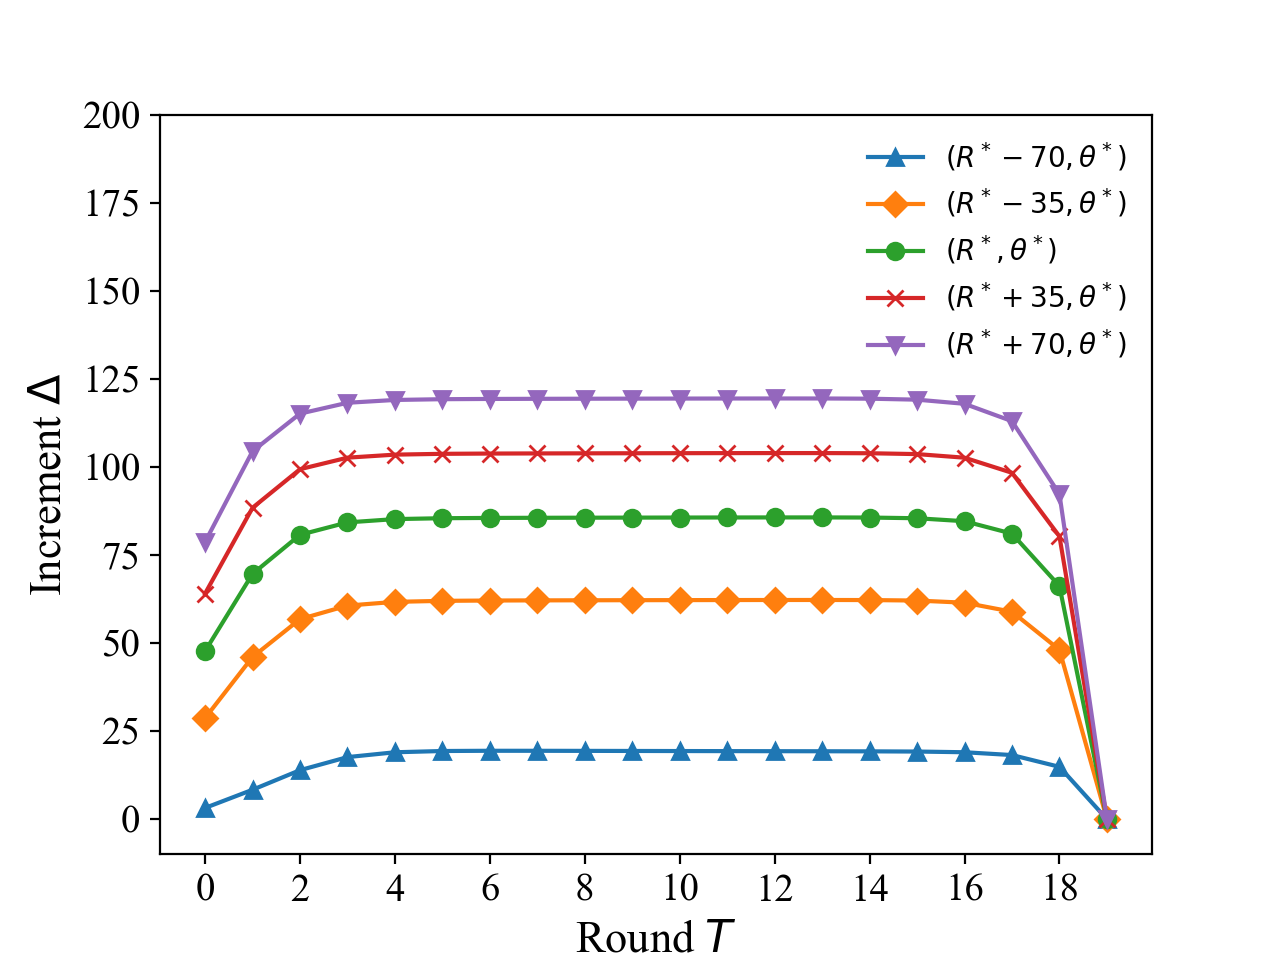
\includegraphics[width=\textwidth]{figures/figure_55_A.png}}
	\end{minipage}
	\begin{minipage}{0.33\linewidth}
		\vspace{3pt}
		\centerline{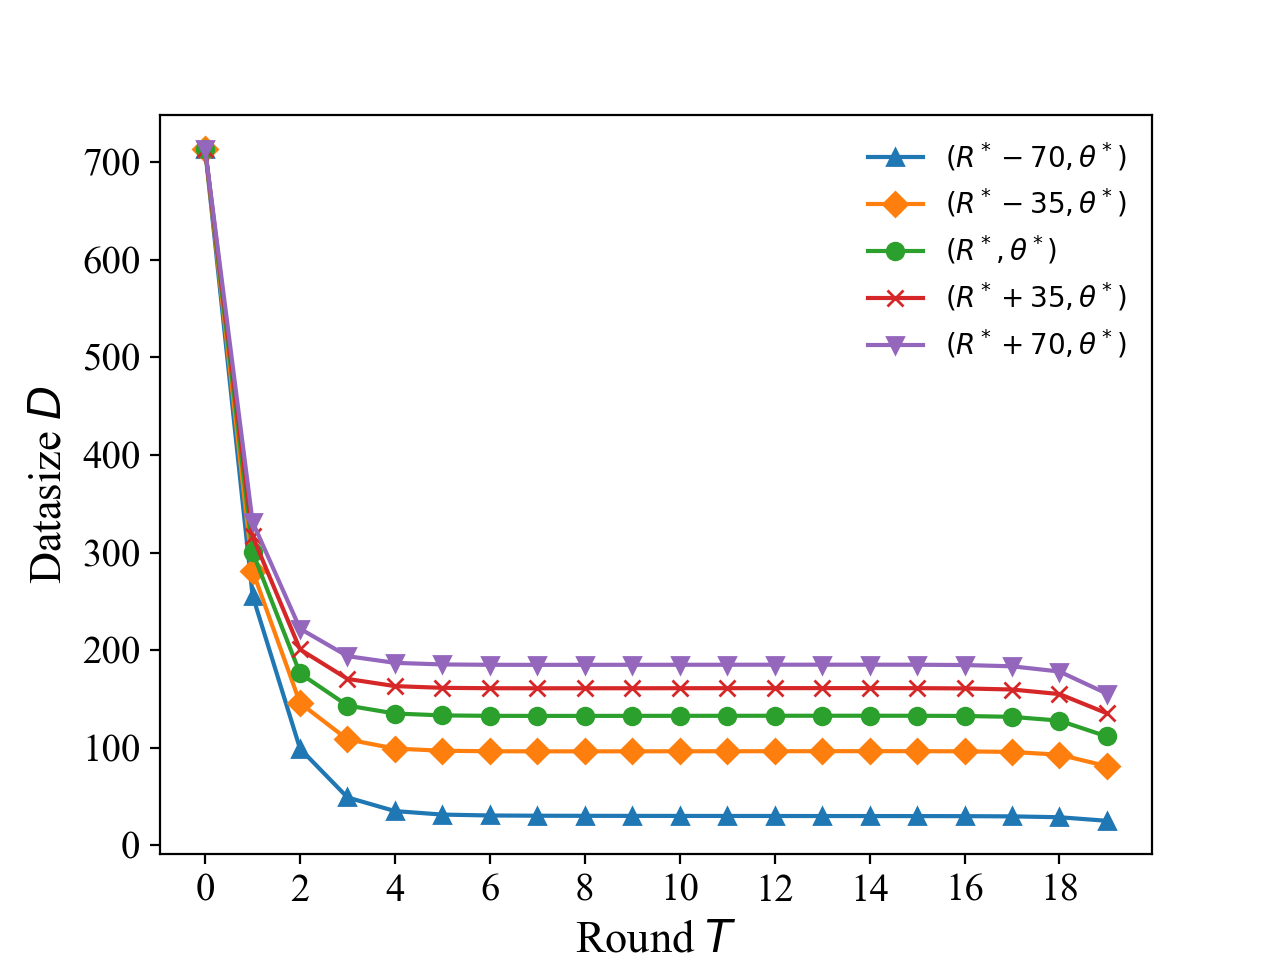
\includegraphics[width=\textwidth]{figures/figure_55_B.png}}
	\end{minipage}
  \begin{minipage}{0.33\linewidth}
		\vspace{3pt}
		\centerline{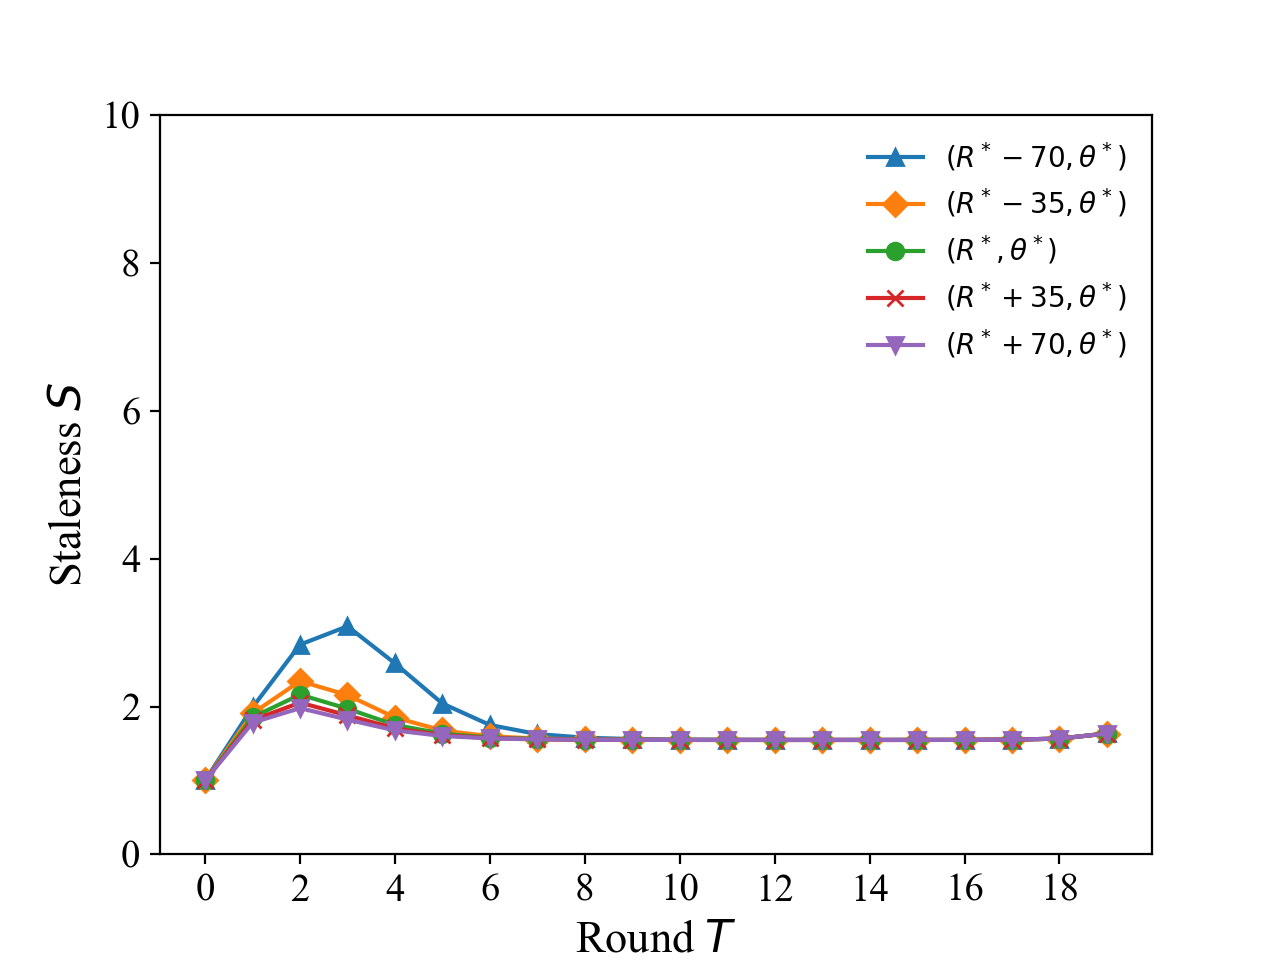
\includegraphics[width=\textwidth]{figures/figure_55_C.png}}
	\end{minipage}
	\caption{The effect of $R$ on data quality and quantity}
\end{figure}

% \textit{Effect of initiative data on server' cost:}
% \begin{figure}
% 	\begin{minipage}{0.33\linewidth}
% 		\vspace{3pt}
%         %这个图片路径替换成你的图片路径即可使用
% 		\centerline{\includegraphics[width=\textwidth]{figures/figure_57_A.png}}
% 	\end{minipage}
% 	\begin{minipage}{0.33\linewidth}
% 		\vspace{3pt}
% 		\centerline{\includegraphics[width=\textwidth]{figures/figure_57_B.png}}
% 	\end{minipage}
%   \begin{minipage}{0.33\linewidth}
% 		\vspace{3pt}
% 		\centerline{\includegraphics[width=\textwidth]{figures/figure_57_C.png}}
% 	\end{minipage}
% 	\caption{The effect of $R$ on model performance}
% \end{figure}

\textit{Effect of initiative data on server' cost:}
\begin{figure}
	\begin{subfigure}{0.31\textwidth}
		\centering
    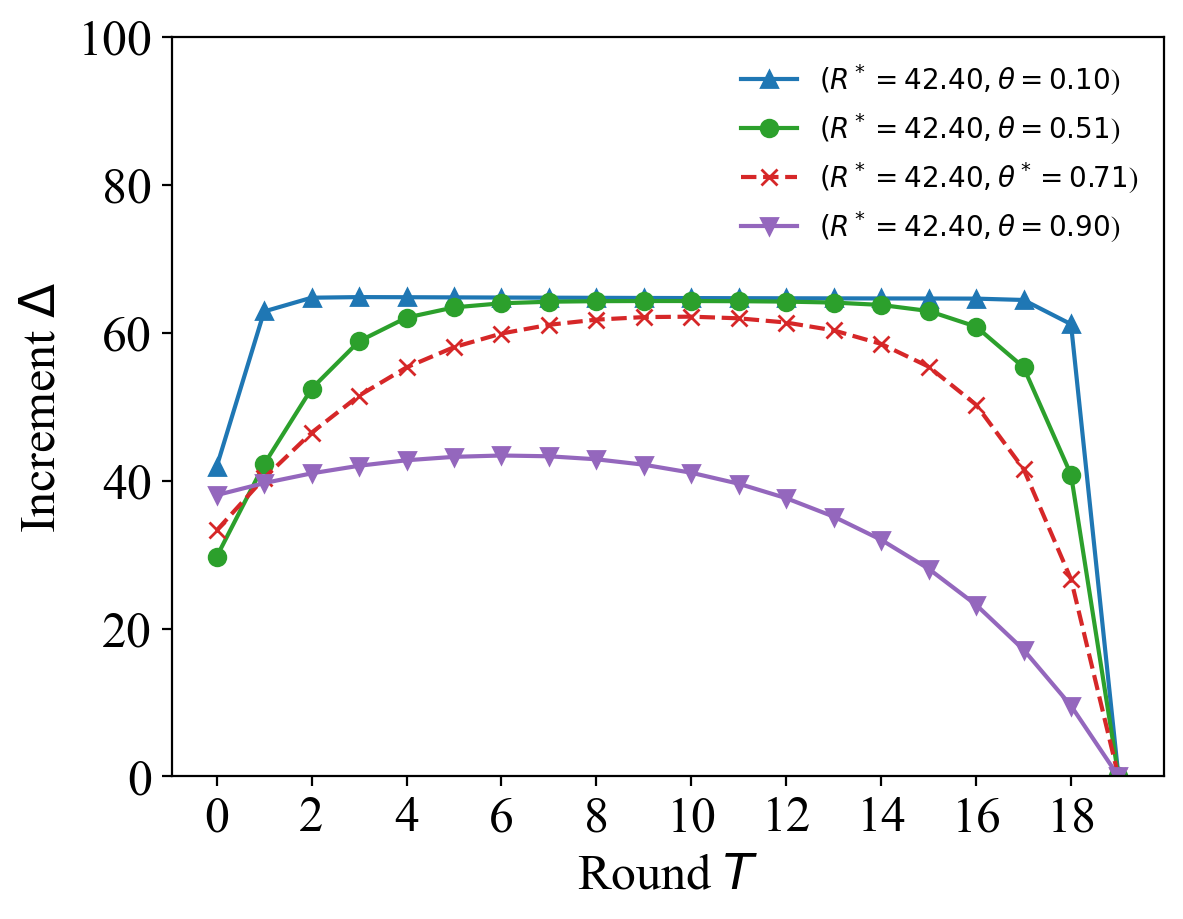
\includegraphics[width=\textwidth]{figures/figure_62_A.png}
    \caption{$\sigma=0.1$}
	\end{subfigure}
  \quad
	\begin{subfigure}{0.31\textwidth}
		\centering
		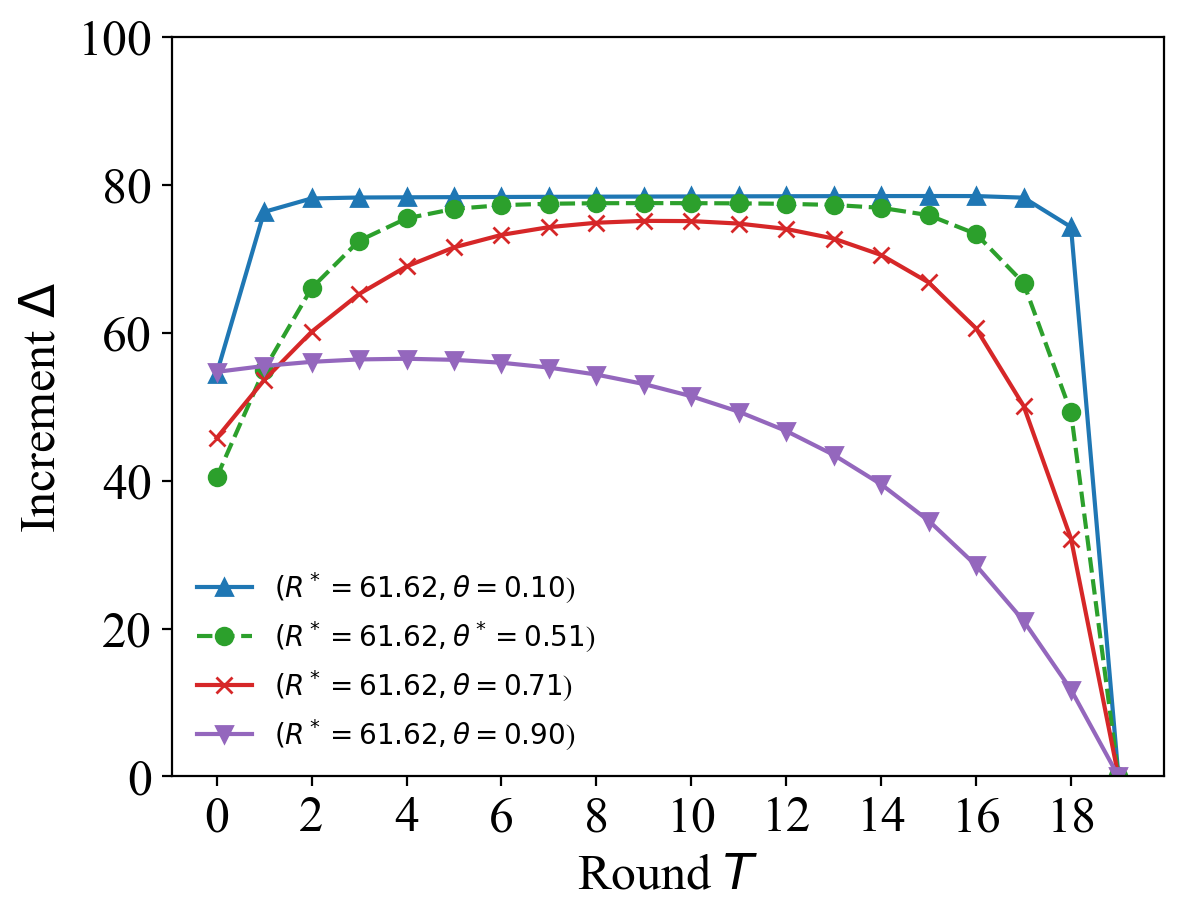
\includegraphics[width=\textwidth]{figures/figure_62_B.png}
    \caption{$\sigma=0.3$}
	\end{subfigure}
  \quad
  \begin{subfigure}{0.31\textwidth}
		\centering
		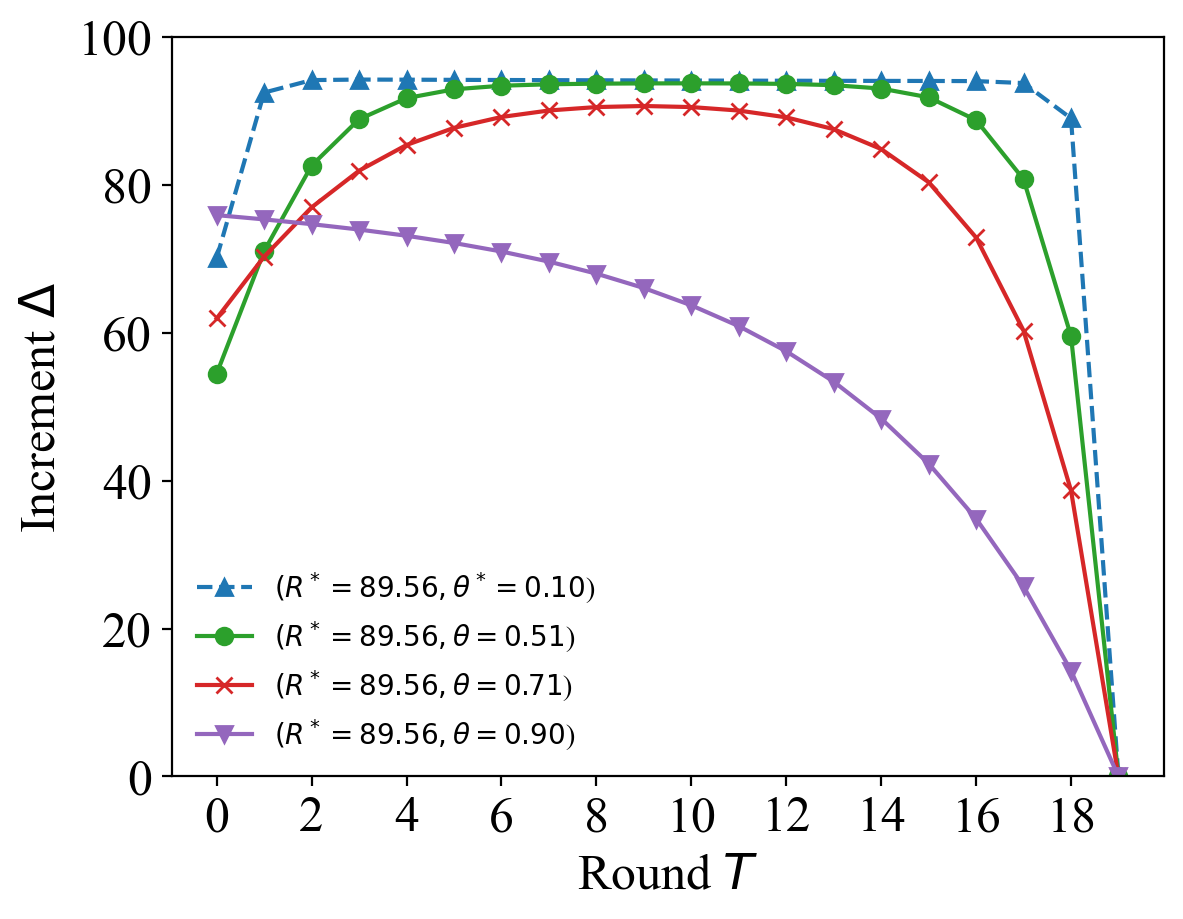
\includegraphics[width=\textwidth]{figures/figure_62_C.png}
    \caption{$\sigma=0.7$}
	\end{subfigure}
	\caption{The effect of $\theta$ on total increment}
\end{figure}

\textit{Effect of initiative data on server' cost:}
\begin{figure}
	\begin{subfigure}{0.31\textwidth}
		\centering
    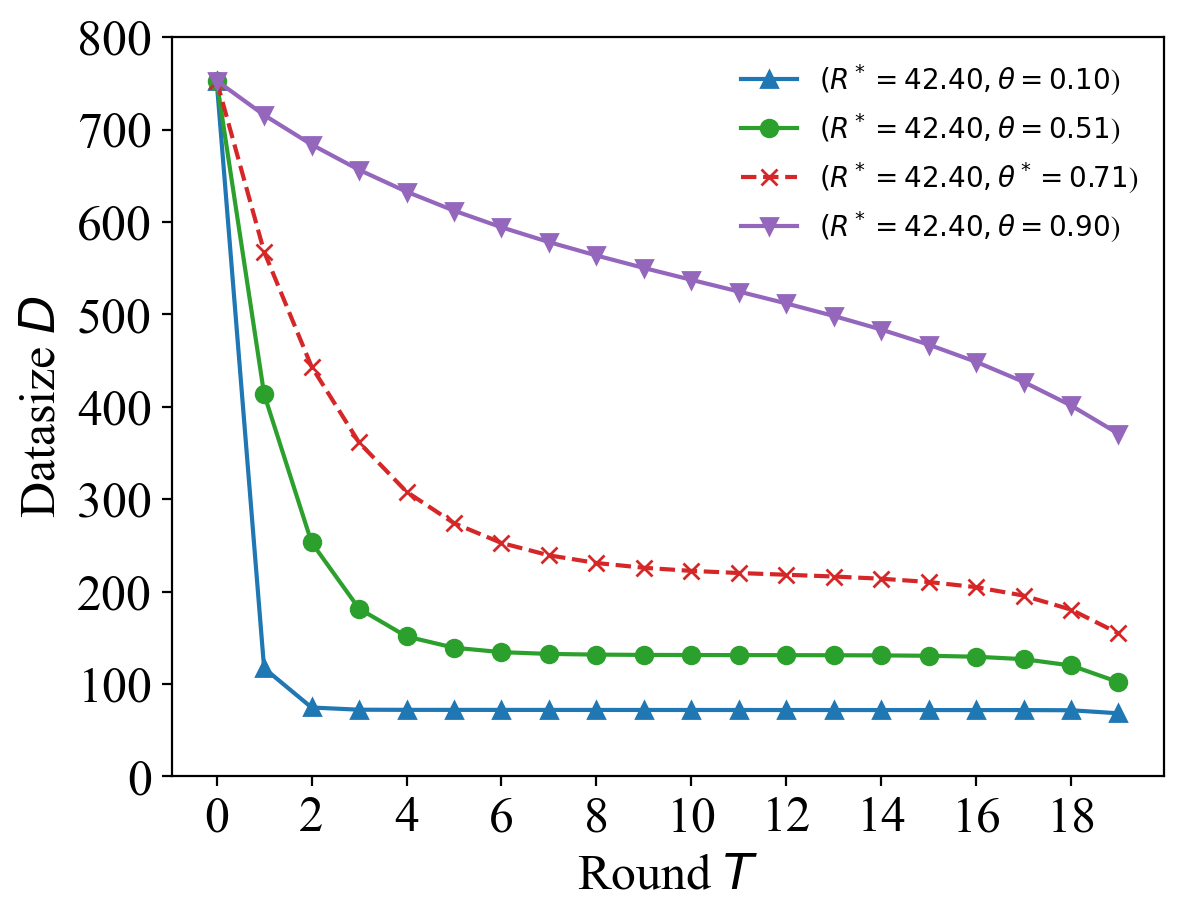
\includegraphics[width=\textwidth]{figures/figure_63_A.png}
    \caption{$\sigma=0.1$}
	\end{subfigure}
  \quad
	\begin{subfigure}{0.31\textwidth}
		\centering
		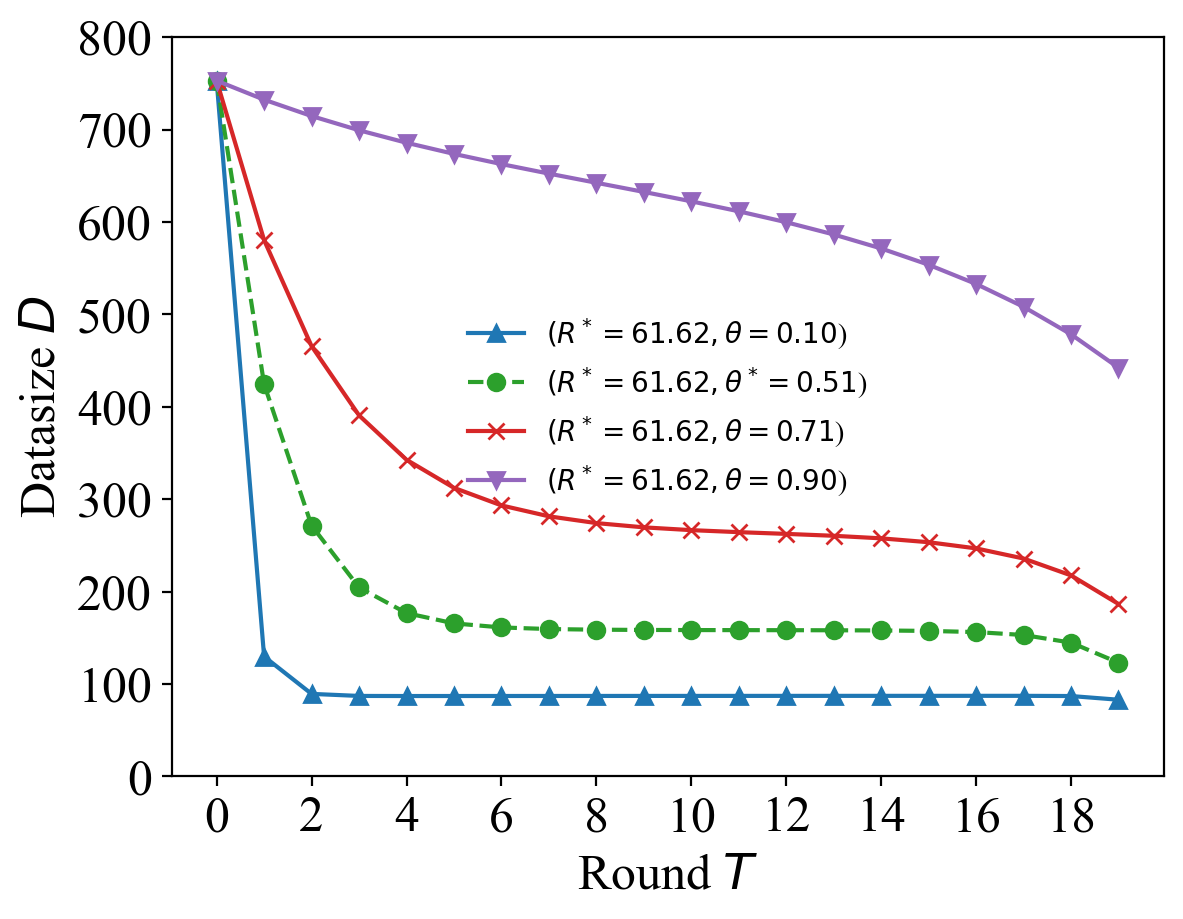
\includegraphics[width=\textwidth]{figures/figure_63_B.png}
    \caption{$\sigma=0.3$}
	\end{subfigure}
  \quad
  \begin{subfigure}{0.31\textwidth}
		\centering
		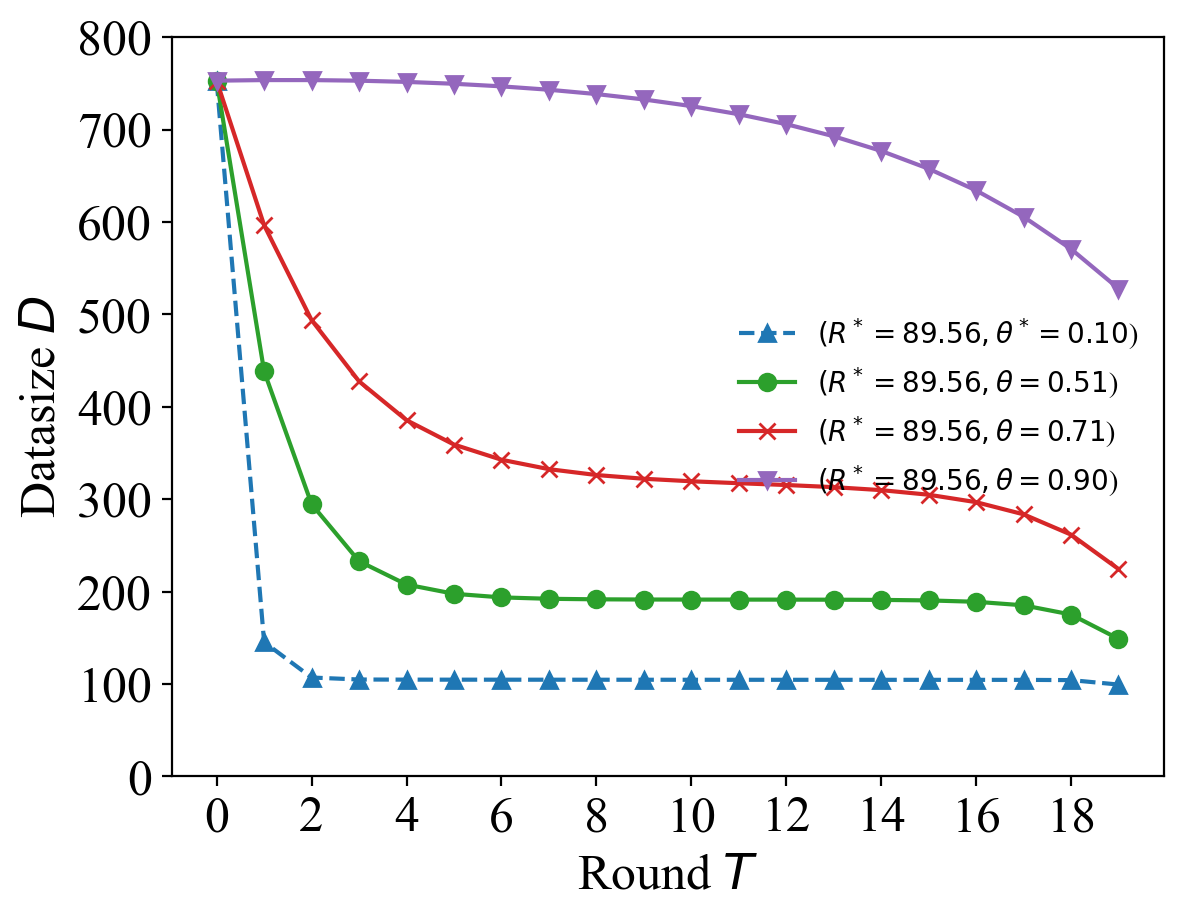
\includegraphics[width=\textwidth]{figures/figure_63_C.png}
    \caption{$\sigma=0.7$}
	\end{subfigure}
	\caption{The effect of $\theta$ on data quantity}
\end{figure}

\textit{Effect of initiative data on server' cost:}
\begin{figure}
	\begin{subfigure}{0.31\textwidth}
		\centering
    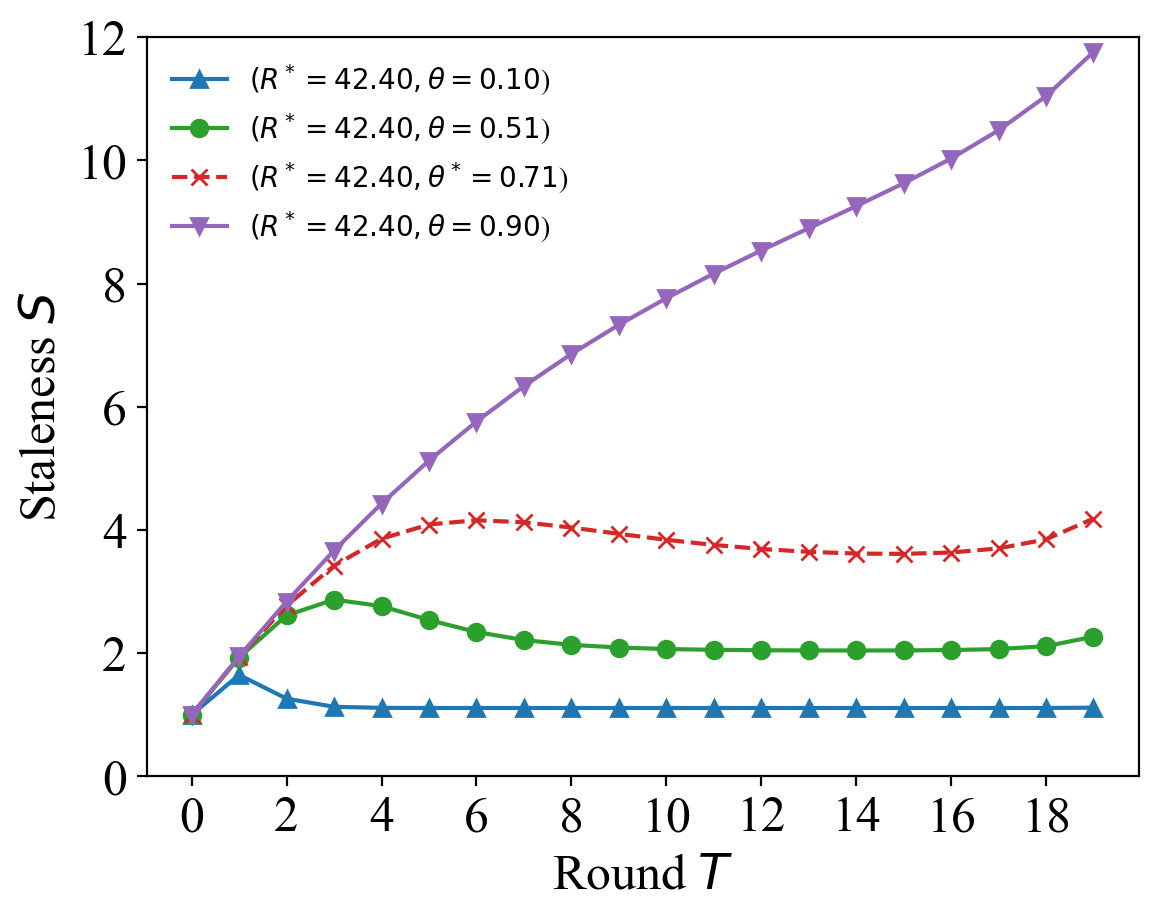
\includegraphics[width=\textwidth]{figures/figure_64_A.png}
    \caption{$\sigma=0.1$}
	\end{subfigure}
  \quad
	\begin{subfigure}{0.31\textwidth}
		\centering
		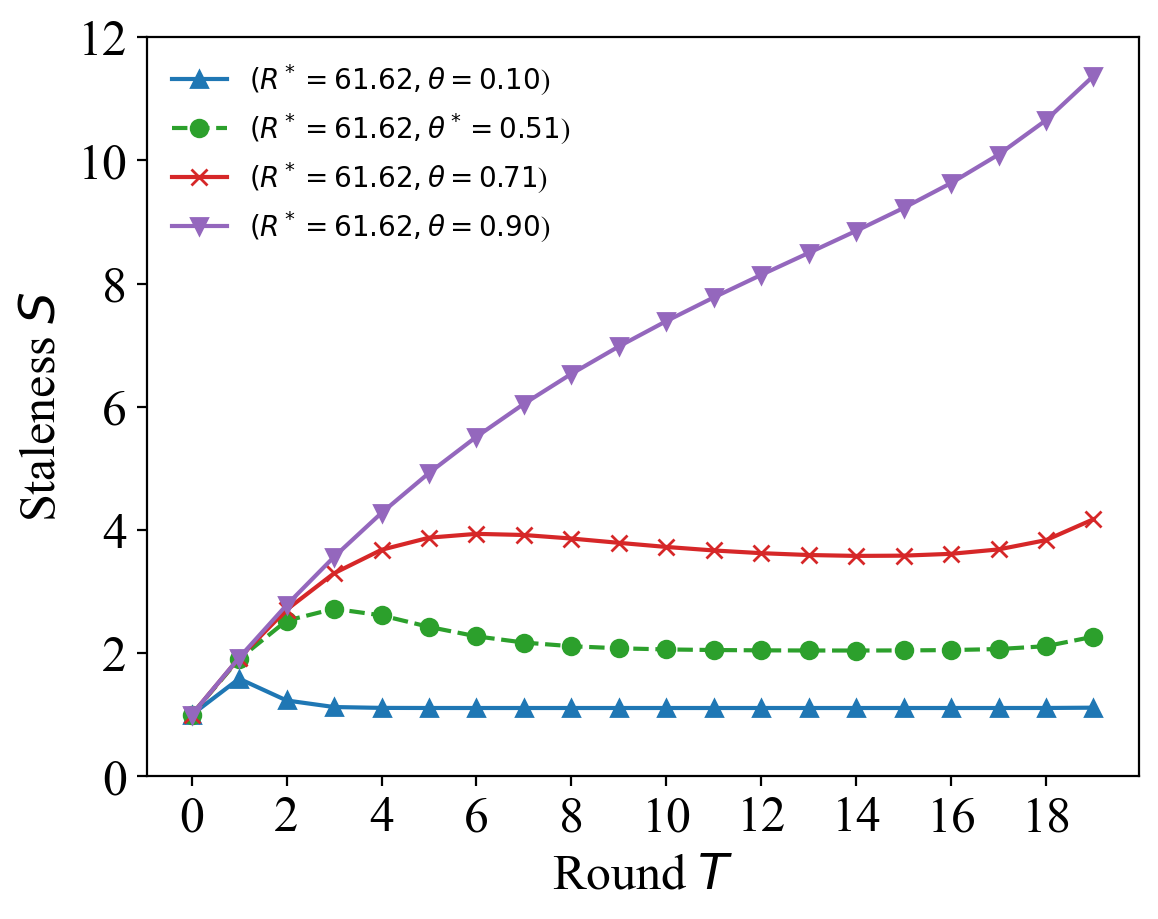
\includegraphics[width=\textwidth]{figures/figure_64_B.png}
    \caption{$\sigma=0.3$}
	\end{subfigure}
  \quad
  \begin{subfigure}{0.31\textwidth}
		\centering
		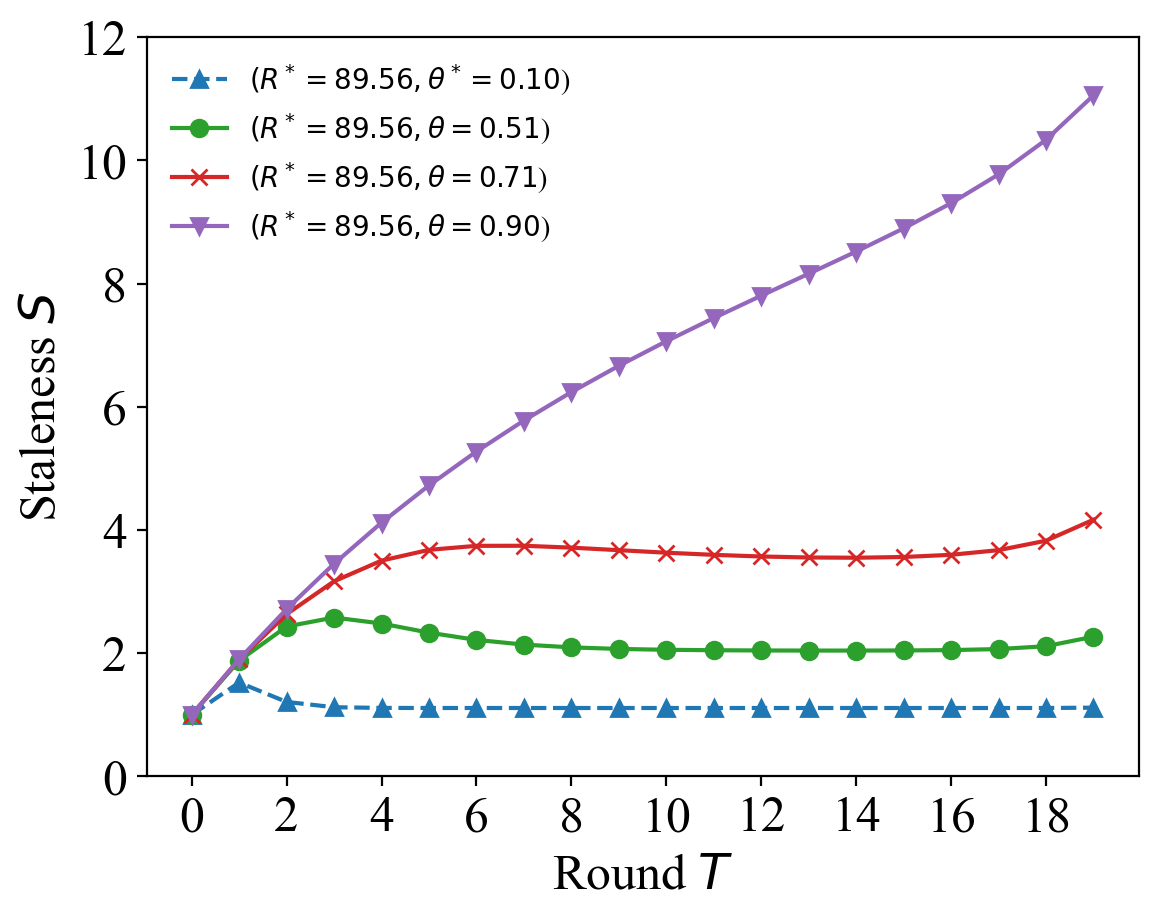
\includegraphics[width=\textwidth]{figures/figure_64_C.png}
    \caption{$\sigma=0.7$}
	\end{subfigure}
	\caption{The effect of $\theta$ on data staleness}
\end{figure}

\textit{Effect of initiative data on server' cost:}
\begin{figure}
	\begin{subfigure}{0.31\textwidth}
		\centering
    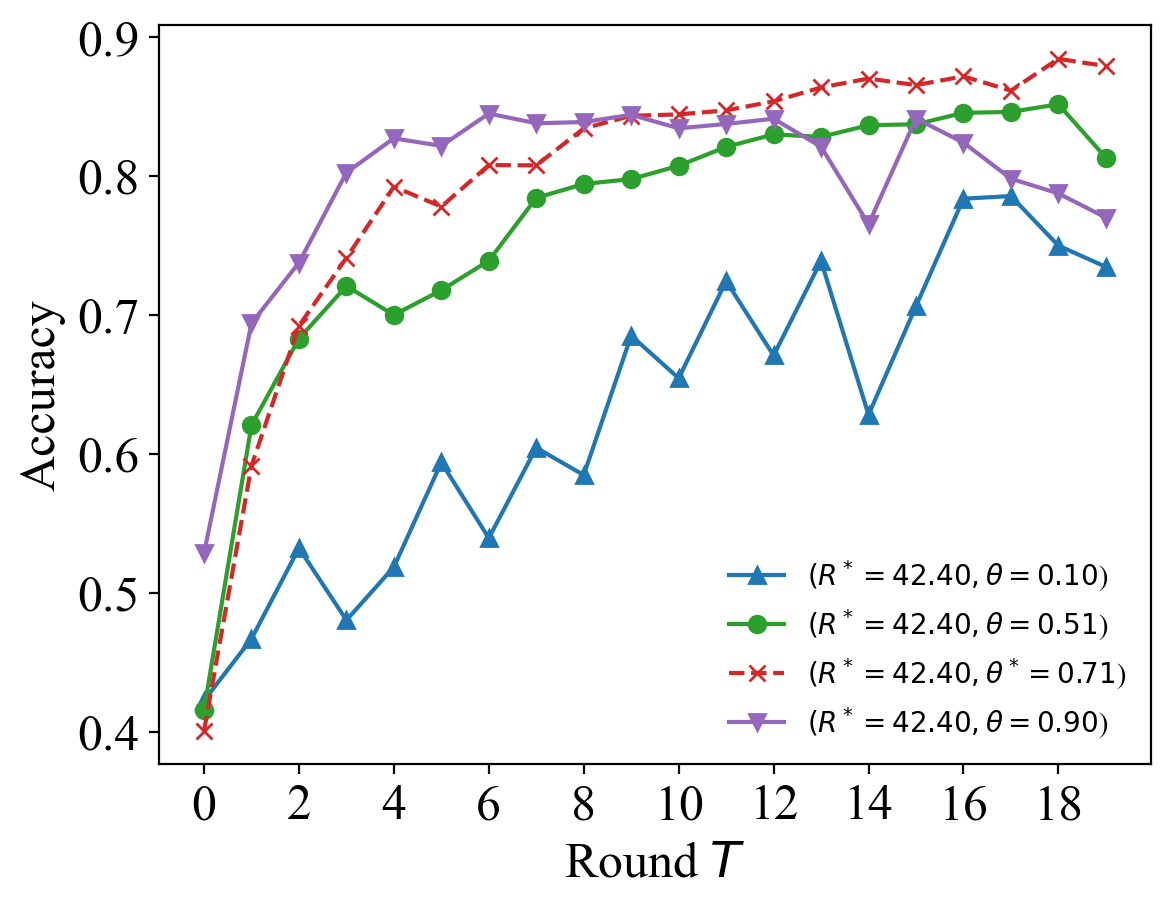
\includegraphics[width=\textwidth]{figures/figure_65_A.png}
    \caption{$\sigma=0.1$}
	\end{subfigure}
  \quad
	\begin{subfigure}{0.31\textwidth}
		\centering
		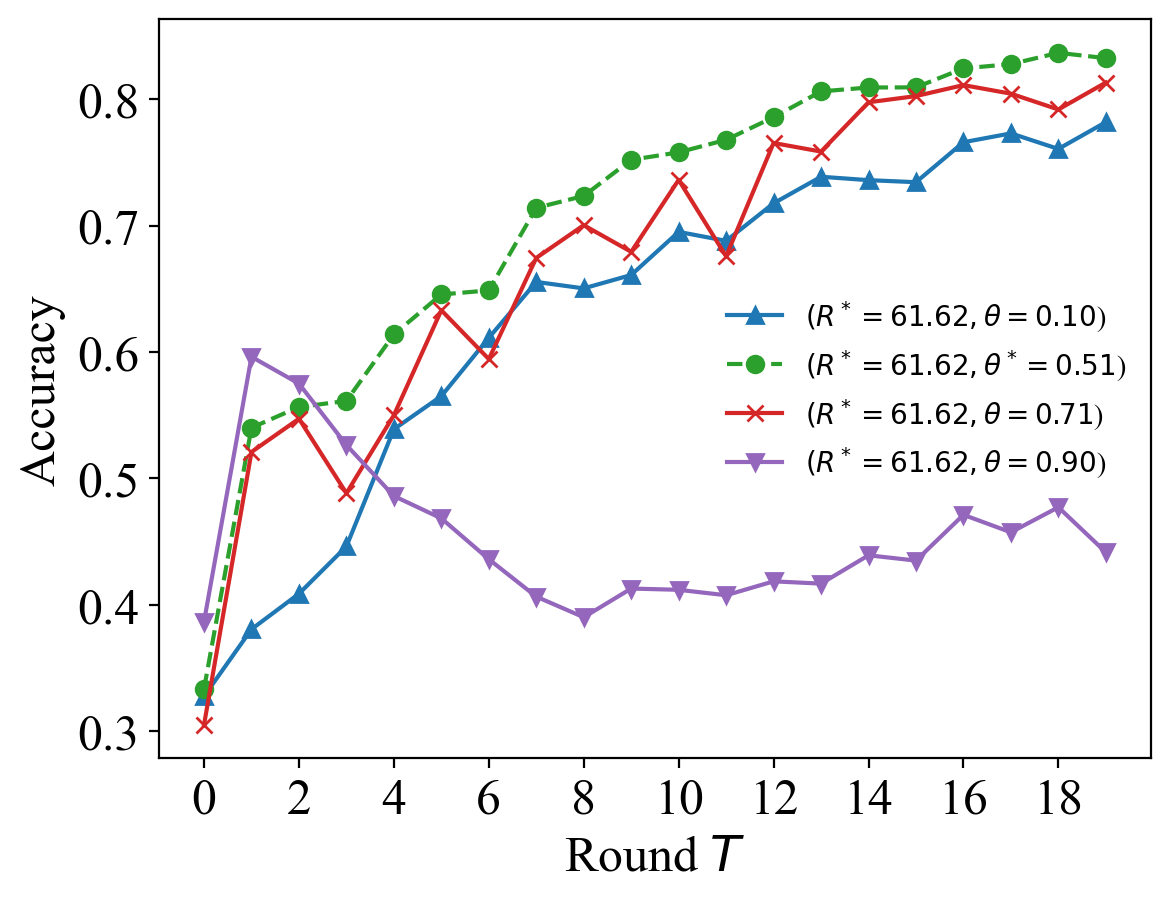
\includegraphics[width=\textwidth]{figures/figure_65_B.png}
    \caption{$\sigma=0.3$}
	\end{subfigure}
  \quad
  \begin{subfigure}{0.31\textwidth}
		\centering
		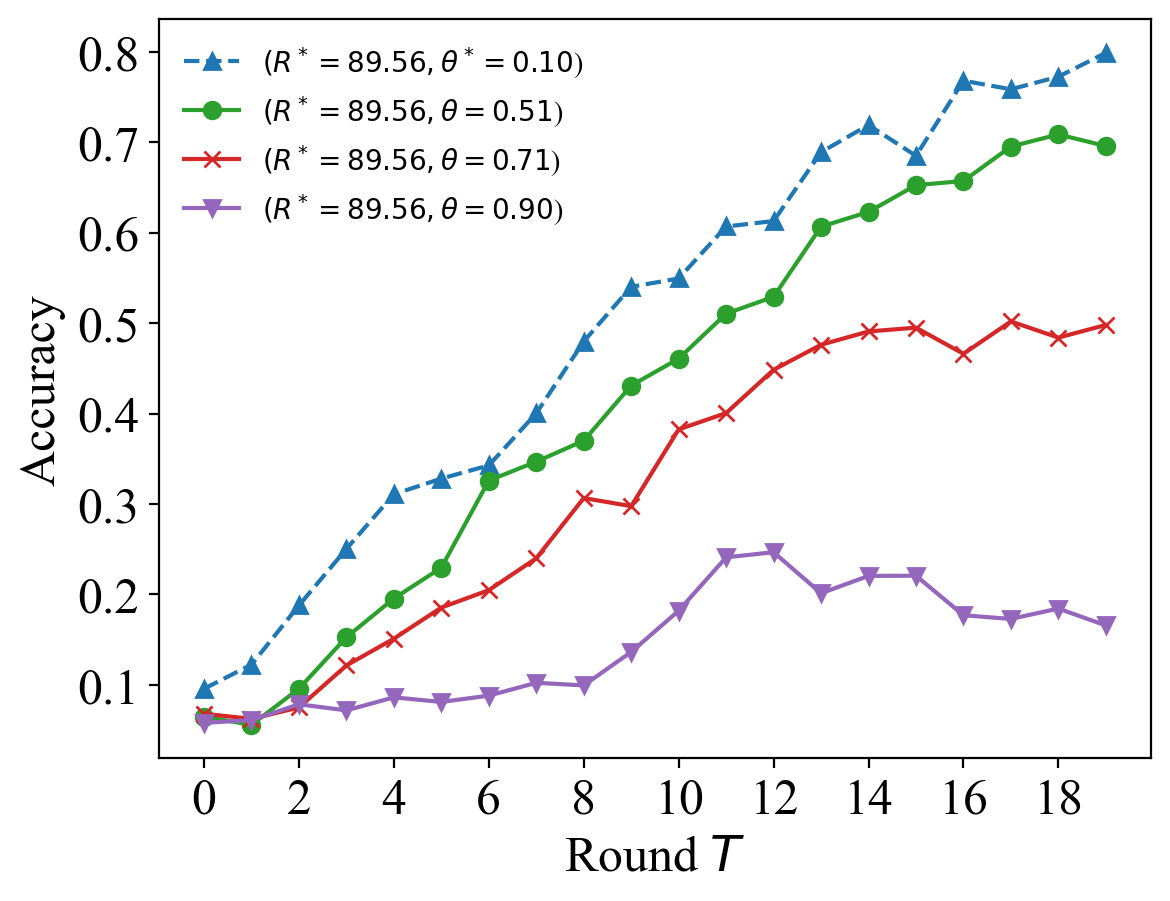
\includegraphics[width=\textwidth]{figures/figure_65_C.png}
    \caption{$\sigma=0.7$}
	\end{subfigure}
	\caption{The effect of $\theta$ on model performance}
\end{figure}

\textit{Effect of initiative data on server' cost:}
\begin{figure}
	\begin{subfigure}{0.31\textwidth}
		\centering
    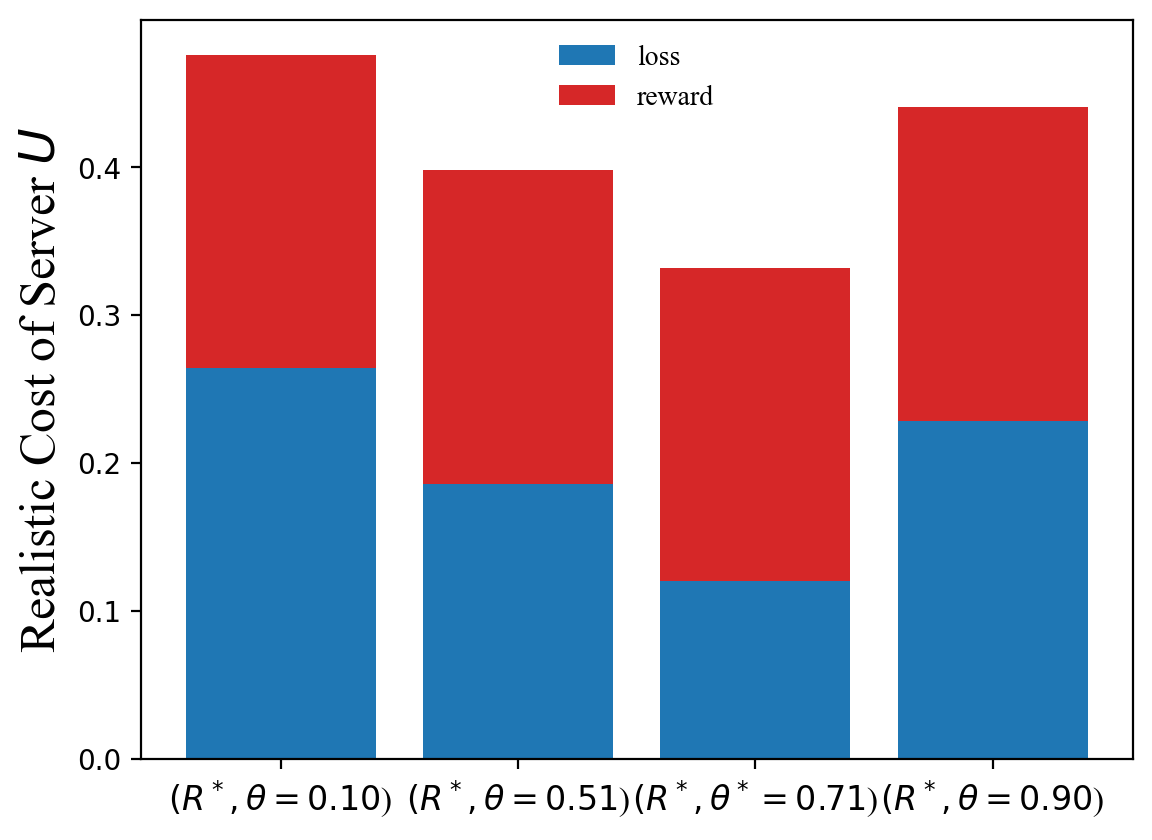
\includegraphics[width=\textwidth]{figures/figure_66_A.png}
    \caption{$\sigma=0.1$}
	\end{subfigure}
  \quad
	\begin{subfigure}{0.31\textwidth}
		\centering
		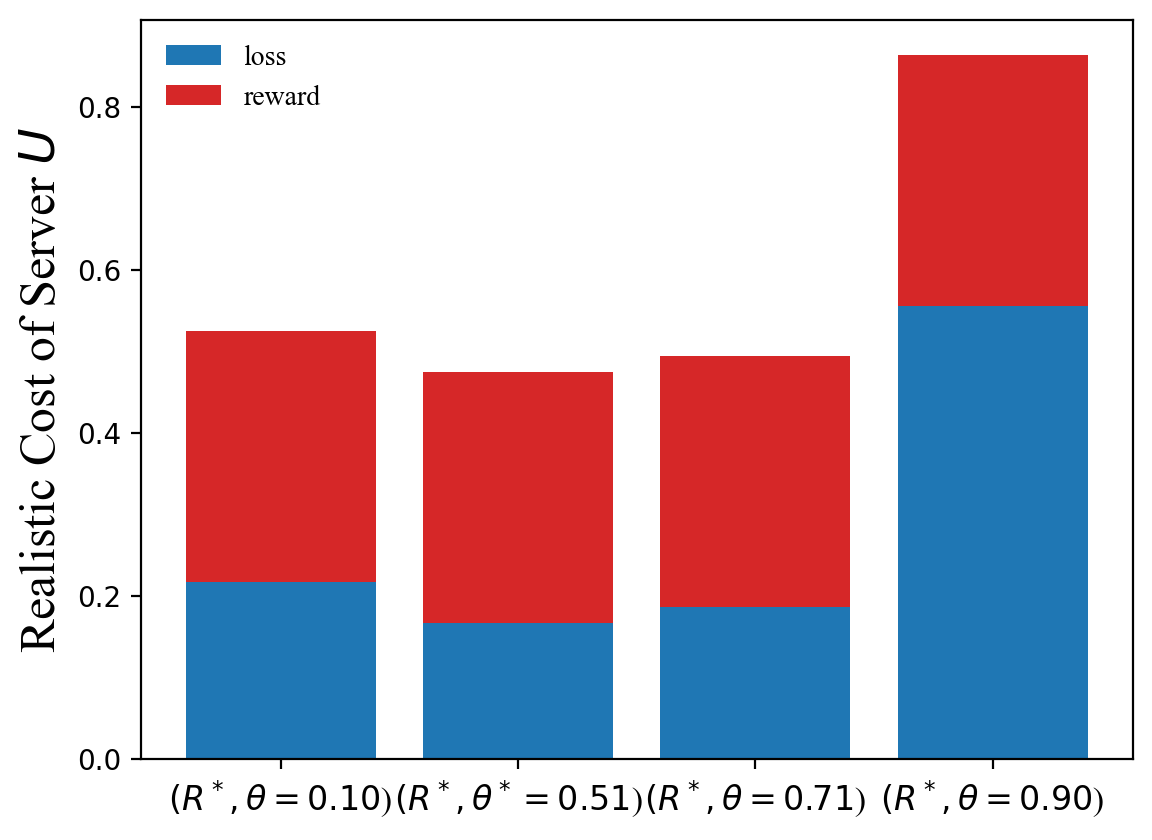
\includegraphics[width=\textwidth]{figures/figure_66_B.png}
    \caption{$\sigma=0.3$}
	\end{subfigure}
  \quad
  \begin{subfigure}{0.31\textwidth}
		\centering
		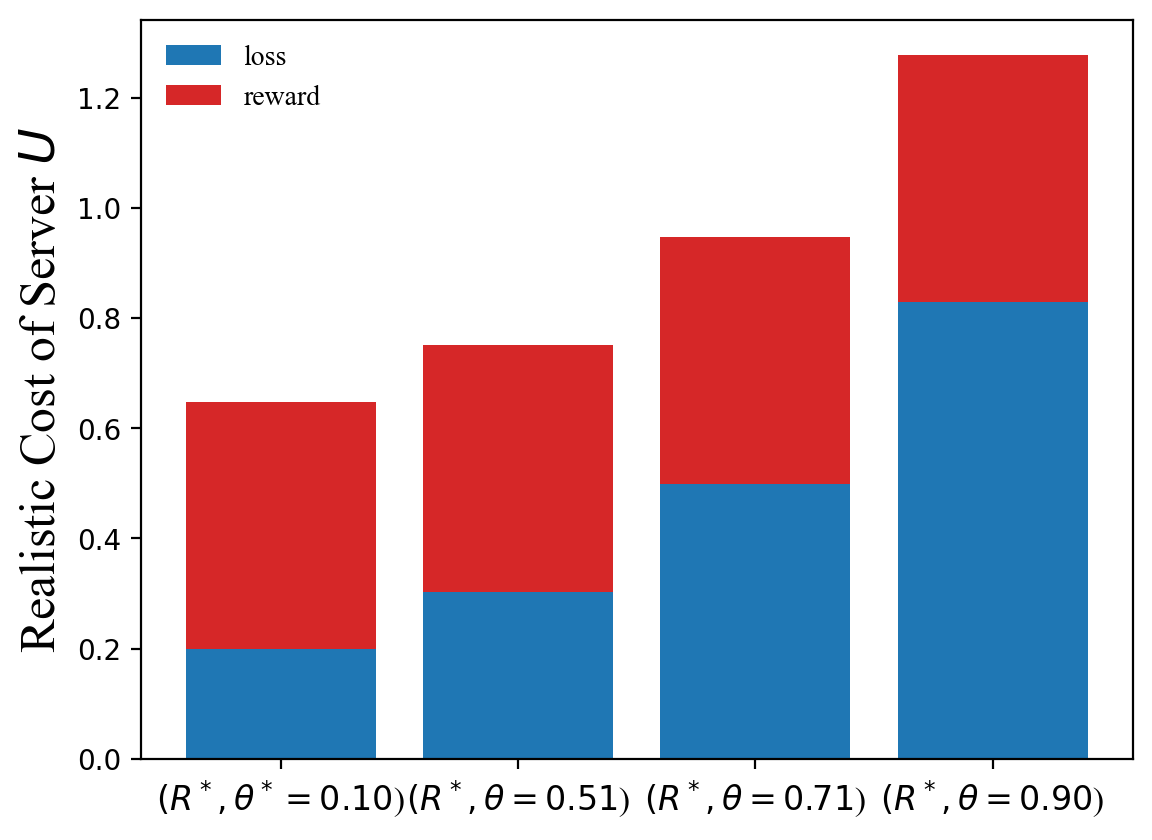
\includegraphics[width=\textwidth]{figures/figure_66_C.png}
    \caption{$\sigma=0.7$}
	\end{subfigure}
	\caption{The effect of $\theta$ on cost}
\end{figure}

\textit{Effect of initiative data on server' cost:}
\begin{figure}
	\begin{subfigure}{0.31\textwidth}
		\centering
    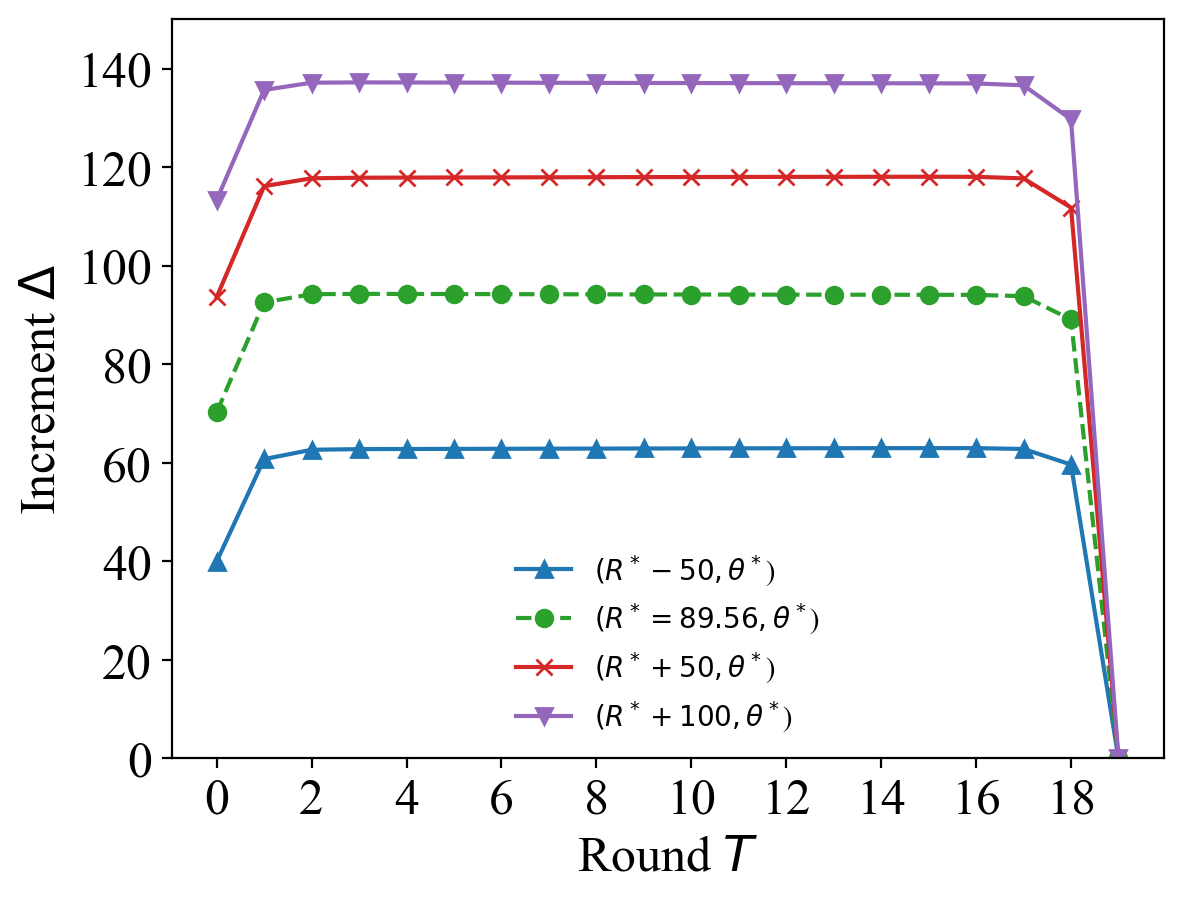
\includegraphics[width=\textwidth]{figures/figure_71_A.png}
    \caption{$\sigma=0.1$}
	\end{subfigure}
  \quad
	\begin{subfigure}{0.31\textwidth}
		\centering
		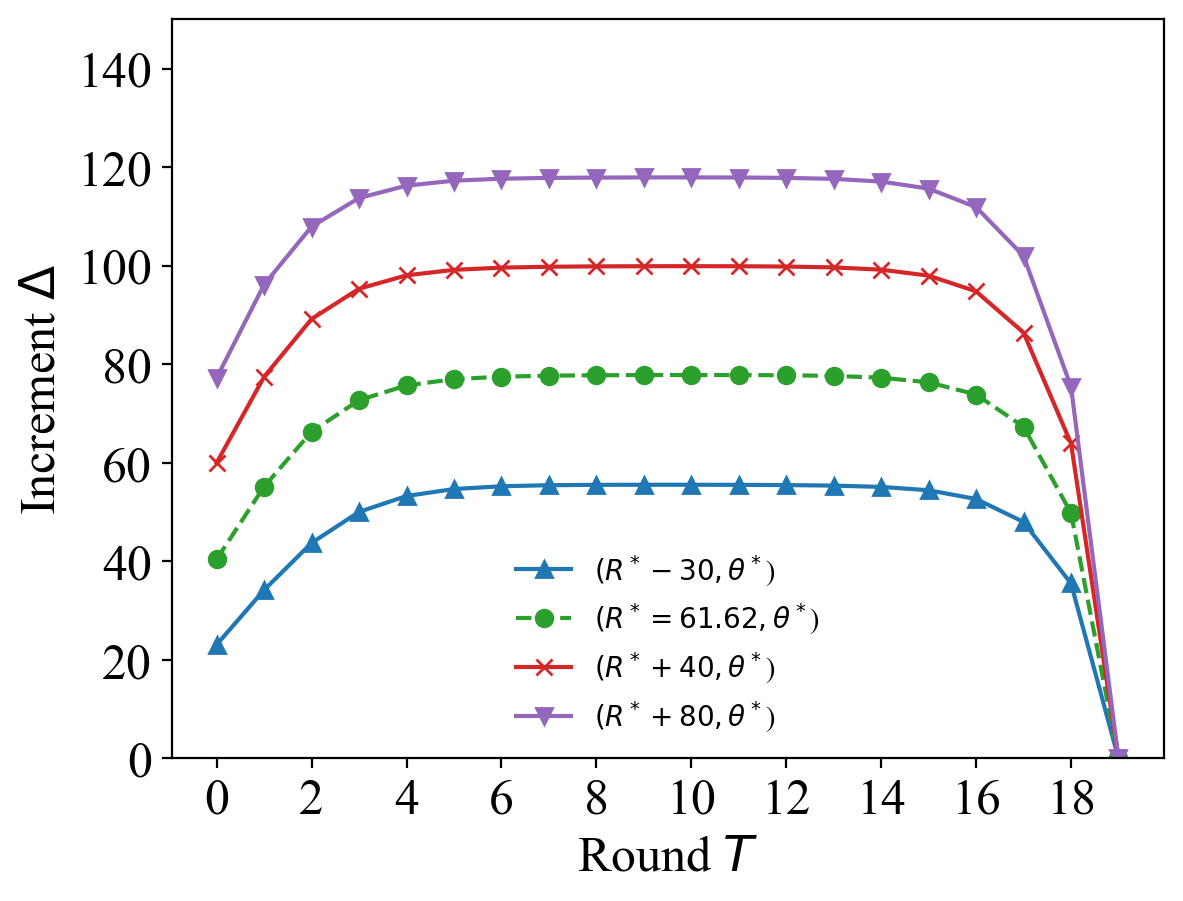
\includegraphics[width=\textwidth]{figures/figure_71_B.png}
    \caption{$\sigma=0.3$}
	\end{subfigure}
  \quad
  \begin{subfigure}{0.31\textwidth}
		\centering
		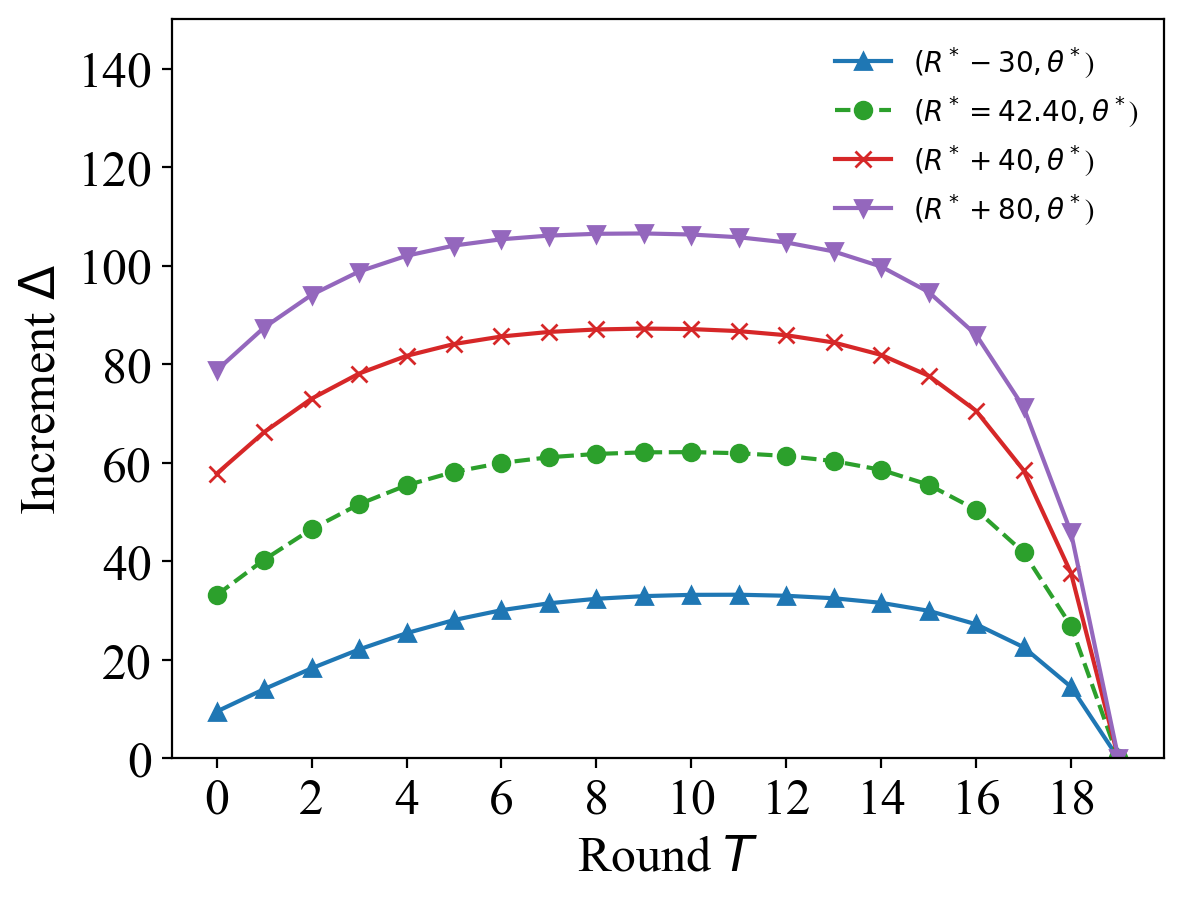
\includegraphics[width=\textwidth]{figures/figure_71_C.png}
    \caption{$\sigma=0.7$}
	\end{subfigure}
	\caption{The effect of $R$ on total increment}
\end{figure}

\textit{Effect of initiative data on server' cost:}
\begin{figure}
	\begin{subfigure}{0.31\textwidth}
		\centering
    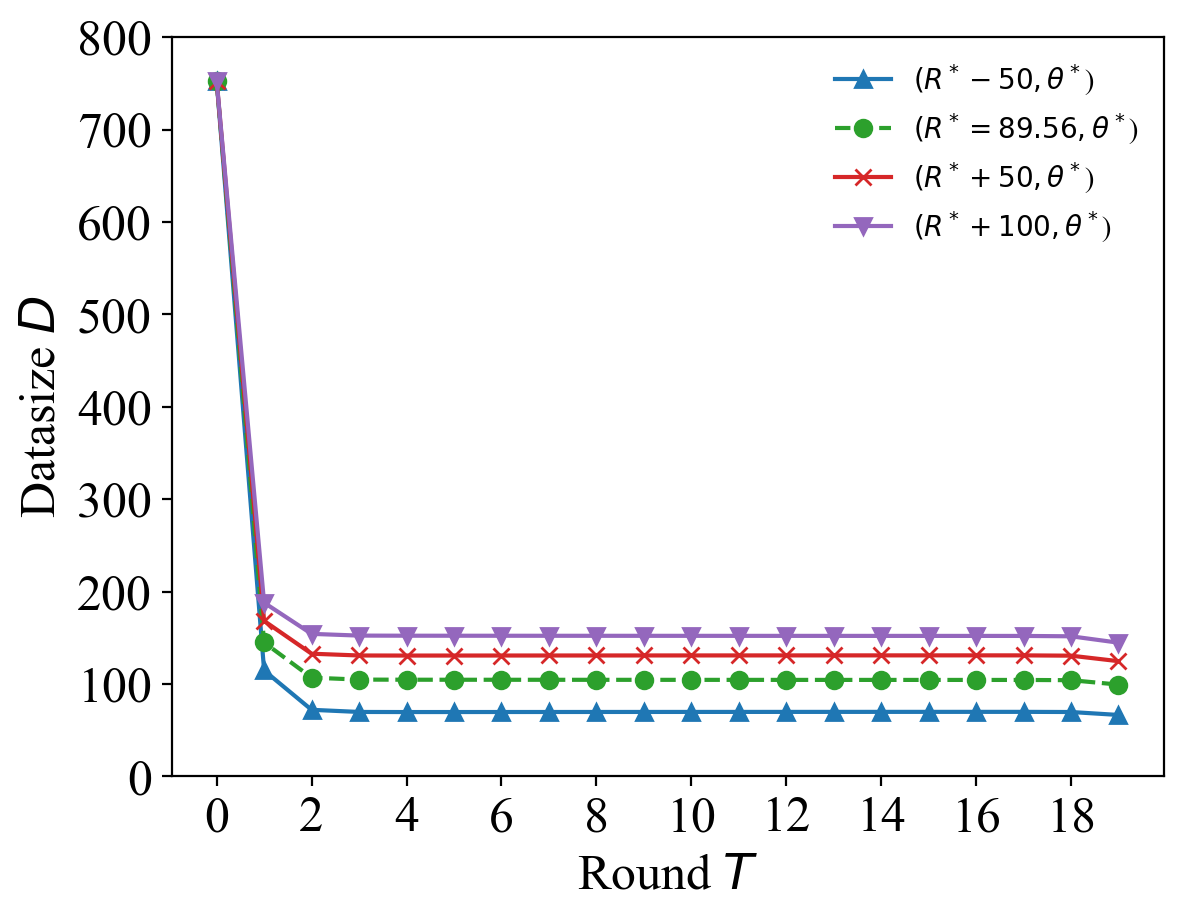
\includegraphics[width=\textwidth]{figures/figure_72_A.png}
    \caption{$\sigma=0.1$}
	\end{subfigure}
  \quad
	\begin{subfigure}{0.31\textwidth}
		\centering
		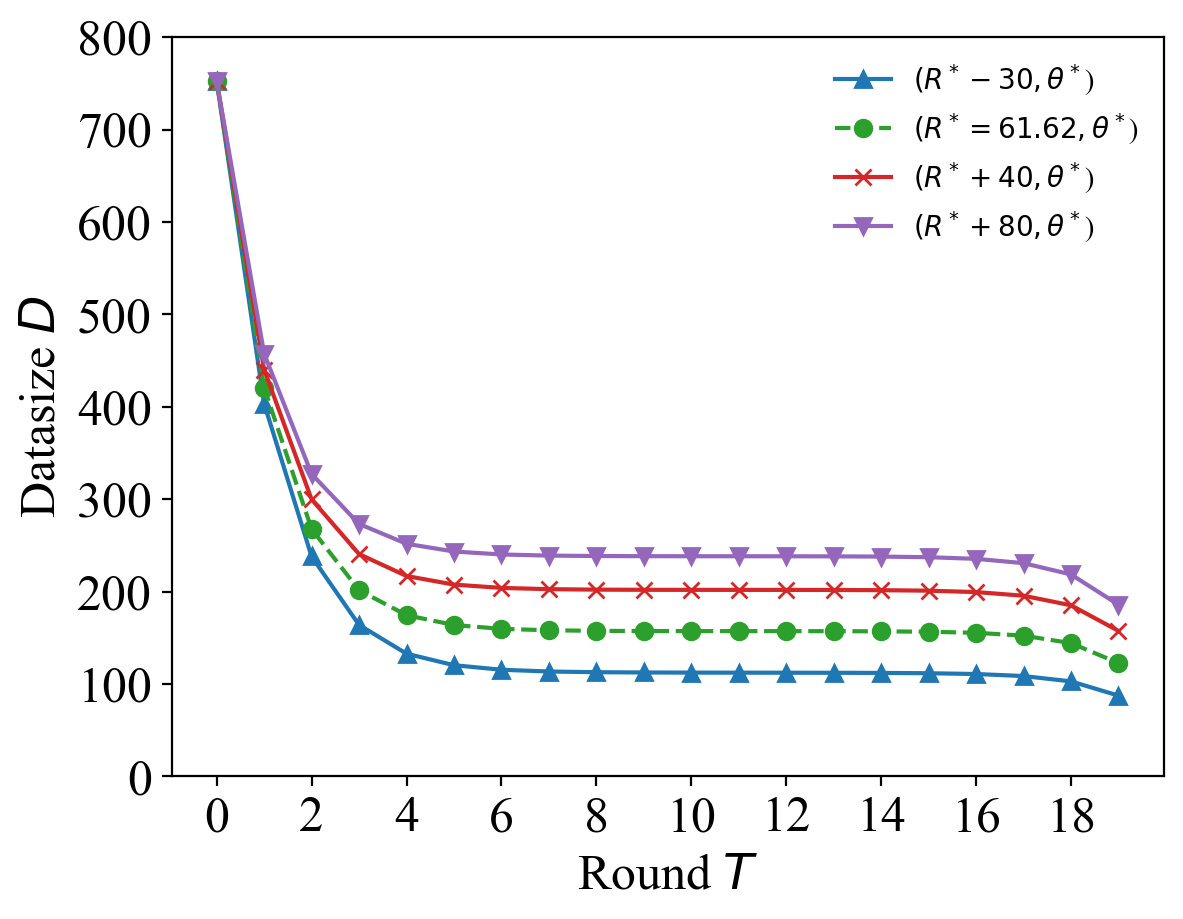
\includegraphics[width=\textwidth]{figures/figure_72_B.png}
    \caption{$\sigma=0.3$}
	\end{subfigure}
  \quad
  \begin{subfigure}{0.31\textwidth}
		\centering
		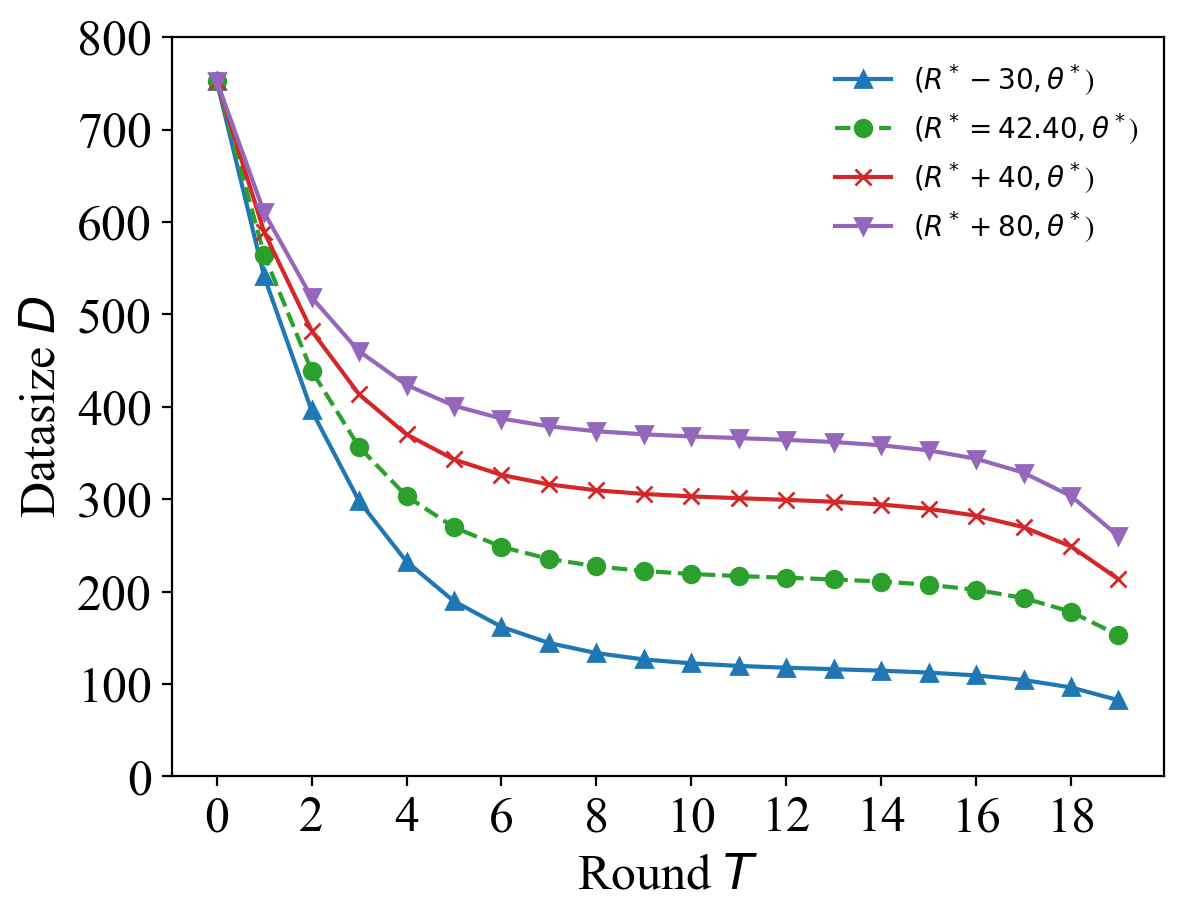
\includegraphics[width=\textwidth]{figures/figure_72_C.png}
    \caption{$\sigma=0.7$}
	\end{subfigure}
	\caption{The effect of $R$ on data quantity}
\end{figure}

\textit{Effect of initiative data on server' cost:}
\begin{figure}
	\begin{subfigure}{0.31\textwidth}
		\centering
    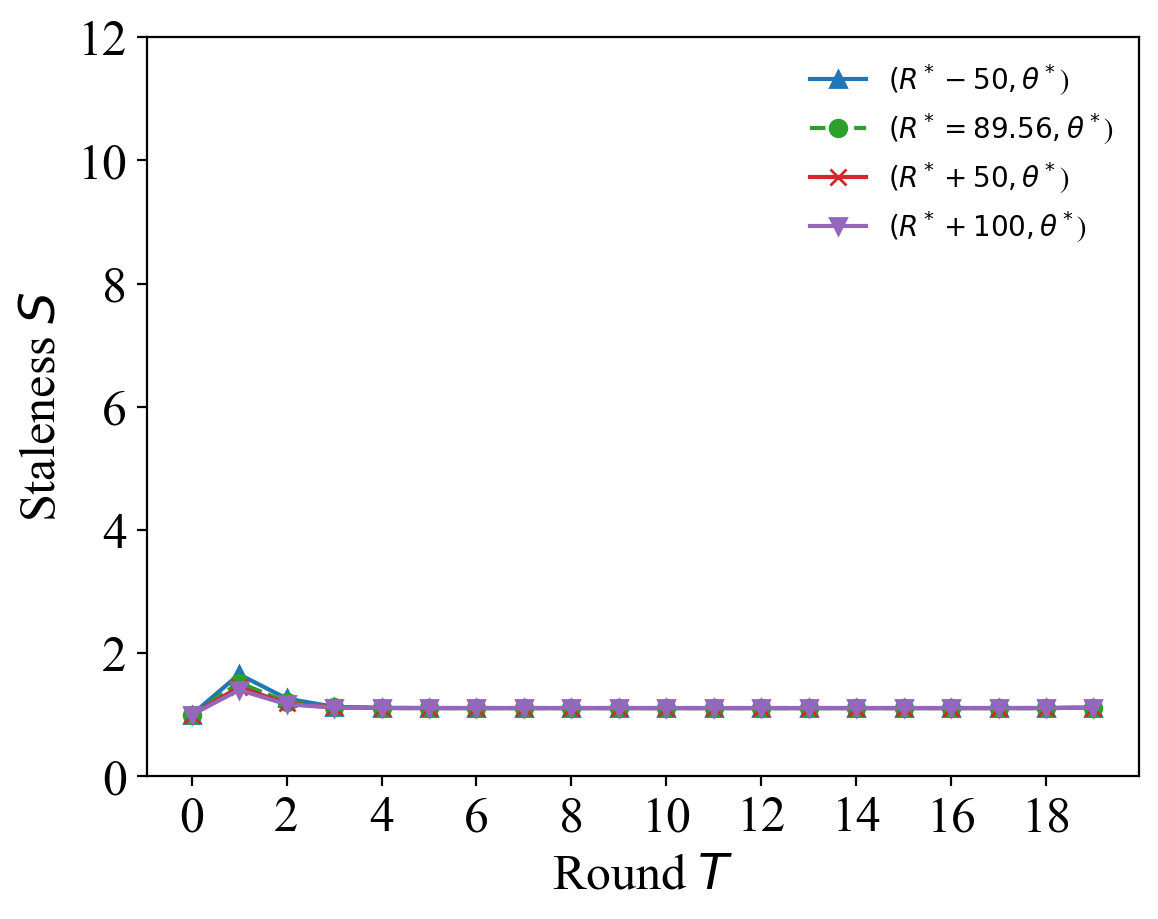
\includegraphics[width=\textwidth]{figures/figure_73_A.png}
    \caption{$\sigma=0.1$}
	\end{subfigure}
  \quad
	\begin{subfigure}{0.31\textwidth}
		\centering
		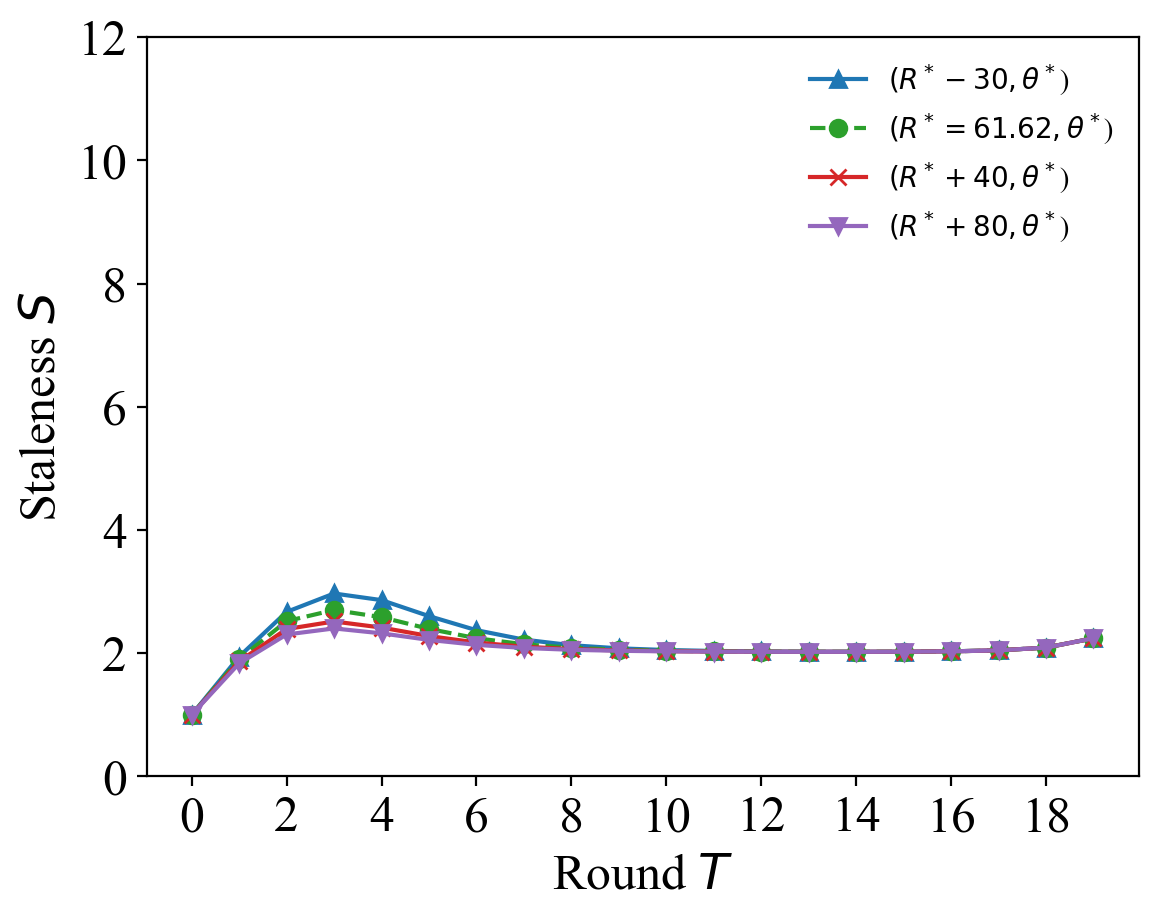
\includegraphics[width=\textwidth]{figures/figure_73_B.png}
    \caption{$\sigma=0.3$}
	\end{subfigure}
  \quad
  \begin{subfigure}{0.31\textwidth}
		\centering
		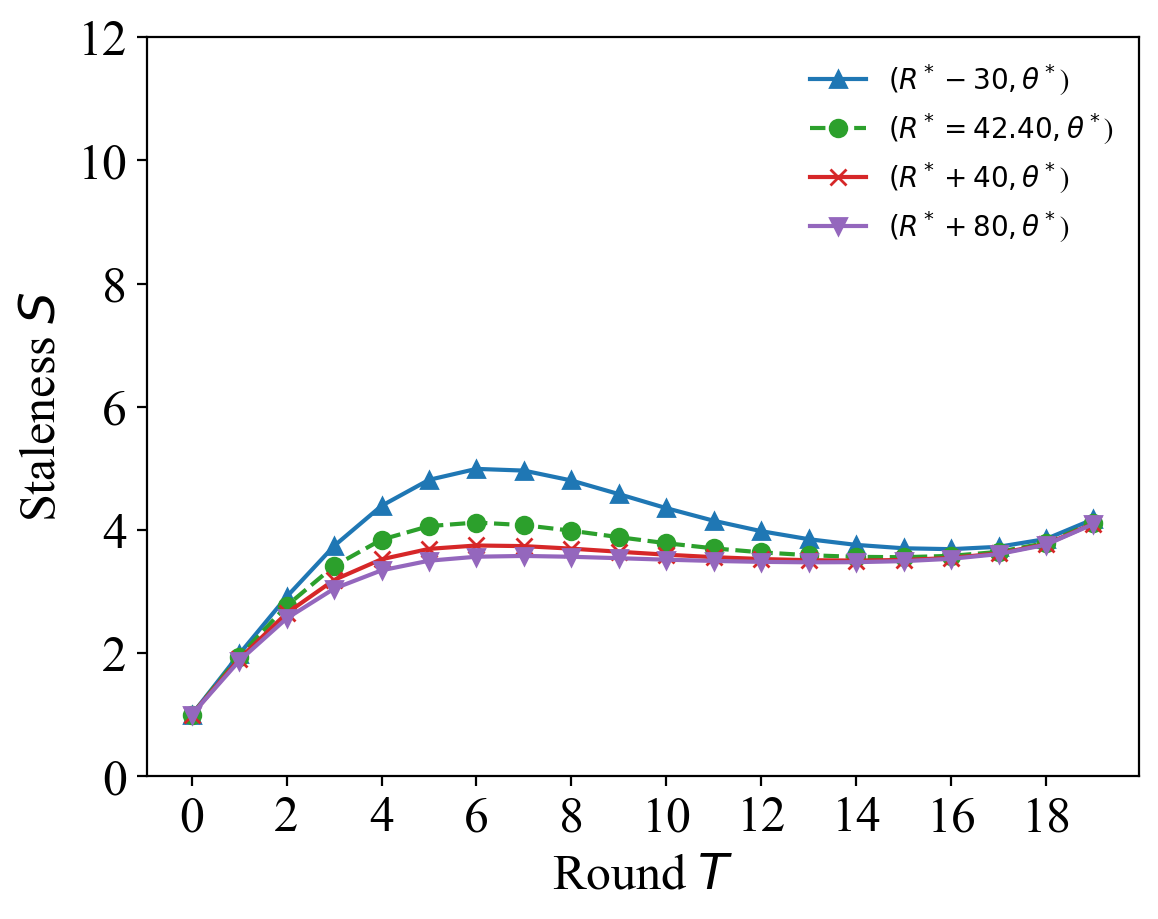
\includegraphics[width=\textwidth]{figures/figure_73_C.png}
    \caption{$\sigma=0.7$}
	\end{subfigure}
	\caption{The effect of $R$ on data staleness}
\end{figure}

\textit{Effect of initiative data on server' cost:}
\begin{figure}
	\begin{subfigure}{0.31\textwidth}
		\centering
    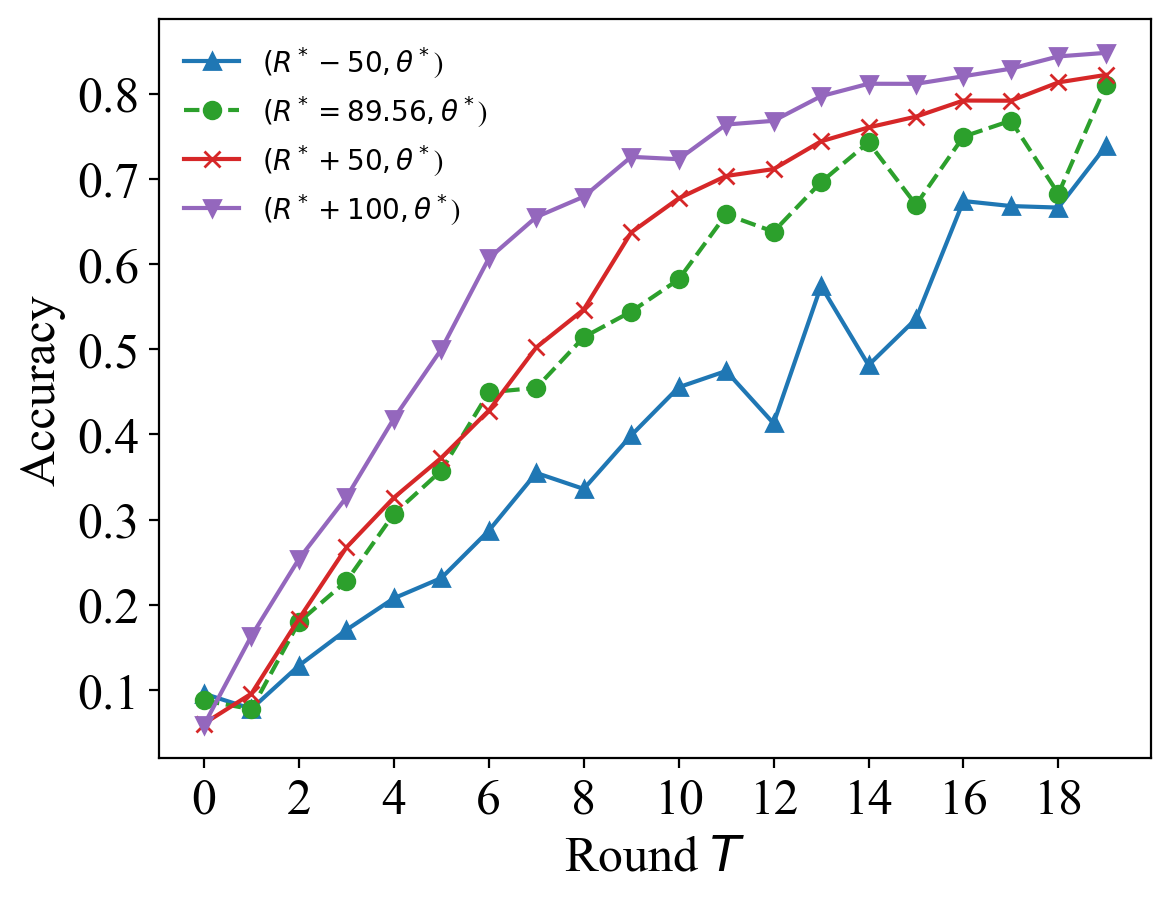
\includegraphics[width=\textwidth]{figures/figure_74_A.png}
    \caption{$\sigma=0.1$}
	\end{subfigure}
  \quad
	\begin{subfigure}{0.31\textwidth}
		\centering
		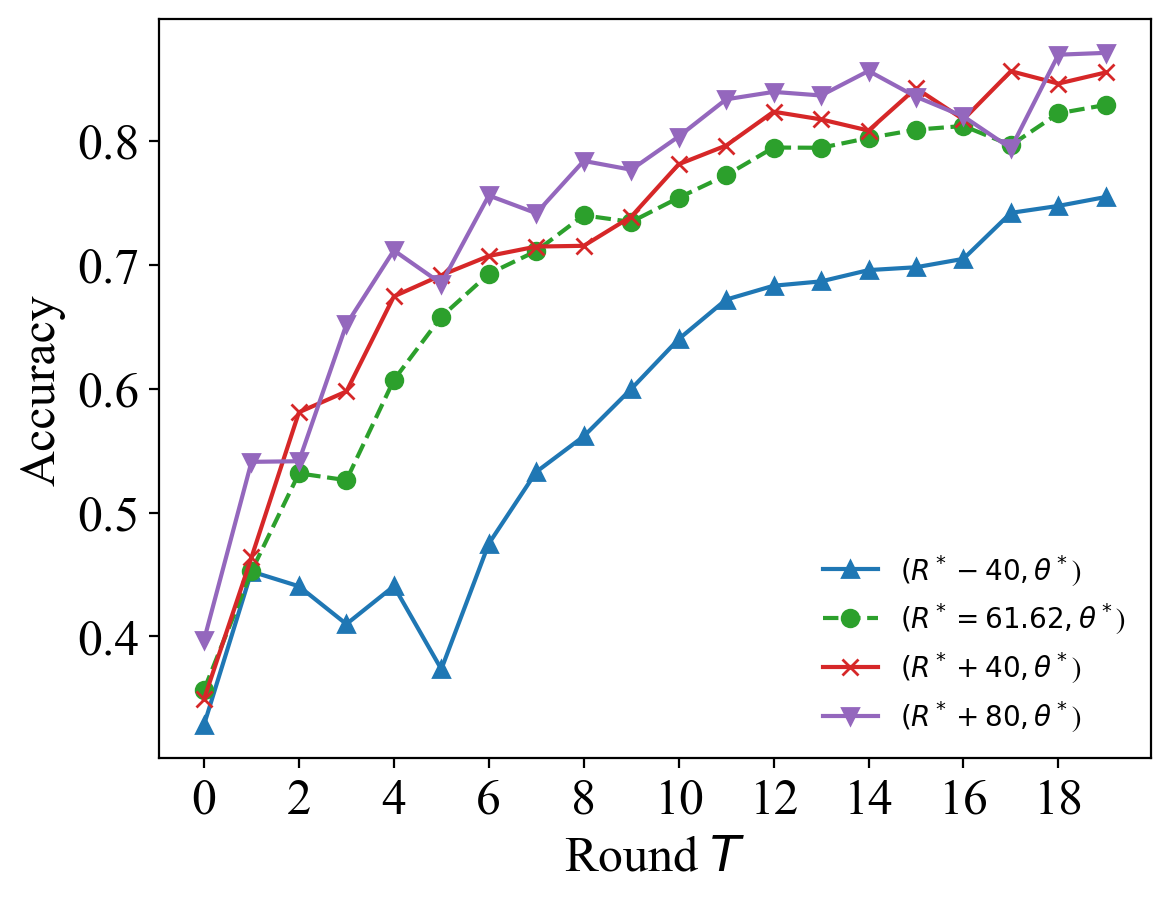
\includegraphics[width=\textwidth]{figures/figure_74_B.png}
    \caption{$\sigma=0.3$}
	\end{subfigure}
  \quad
  \begin{subfigure}{0.31\textwidth}
		\centering
		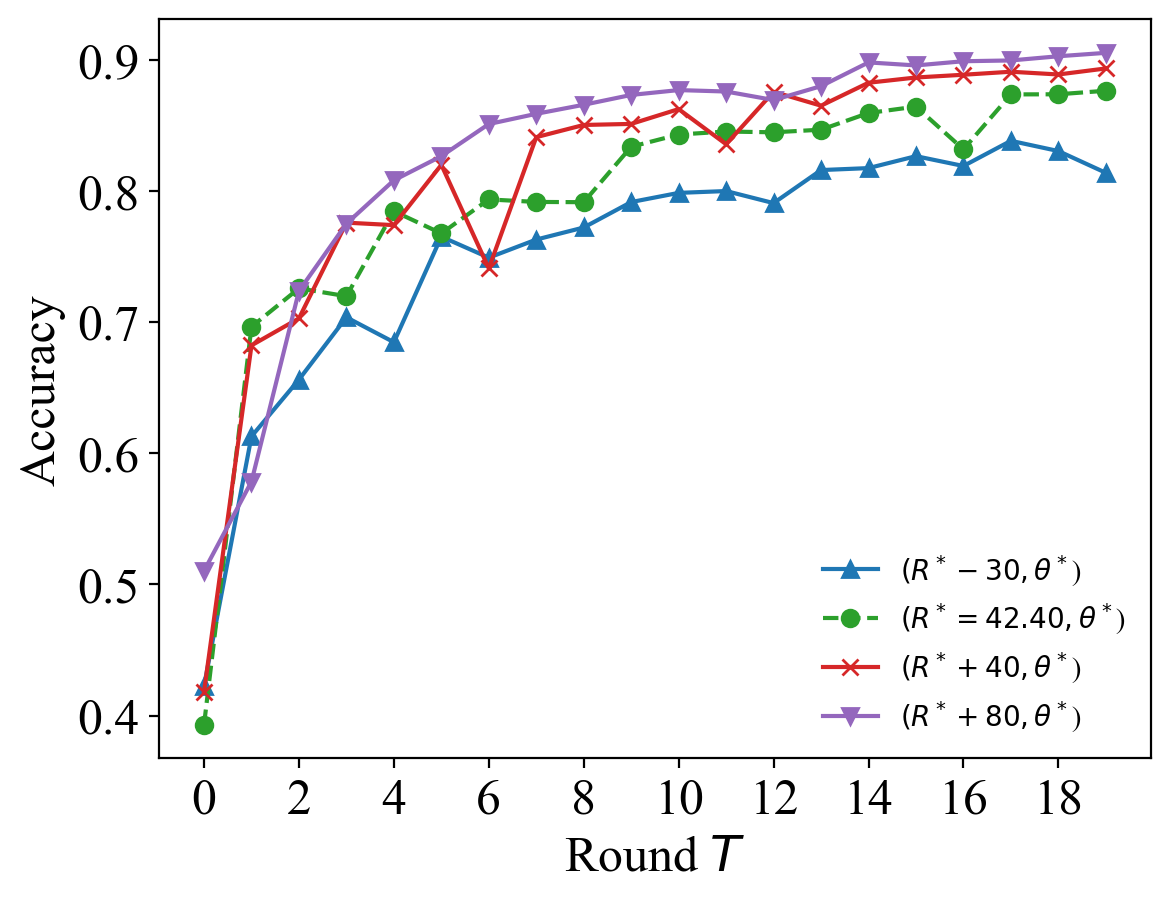
\includegraphics[width=\textwidth]{figures/figure_74_C.png}
    \caption{$\sigma=0.7$}
	\end{subfigure}
	\caption{The effect of $R$ on model performance}
\end{figure}

\textit{Effect of initiative data on server' cost:}
\begin{figure}
	\begin{subfigure}{0.31\textwidth}
		\centering
    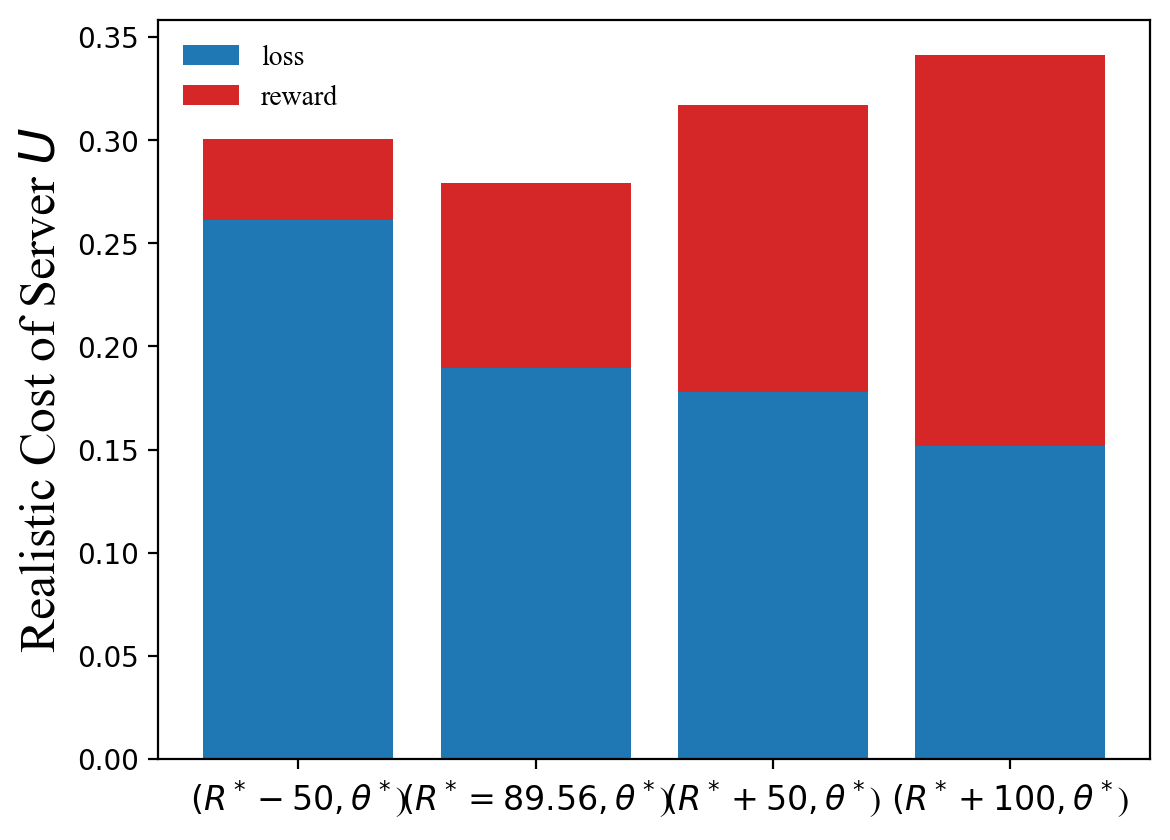
\includegraphics[width=\textwidth]{figures/figure_75_A.png}
    \caption{$\sigma=0.1$}
	\end{subfigure}
  \quad
	\begin{subfigure}{0.31\textwidth}
		\centering
		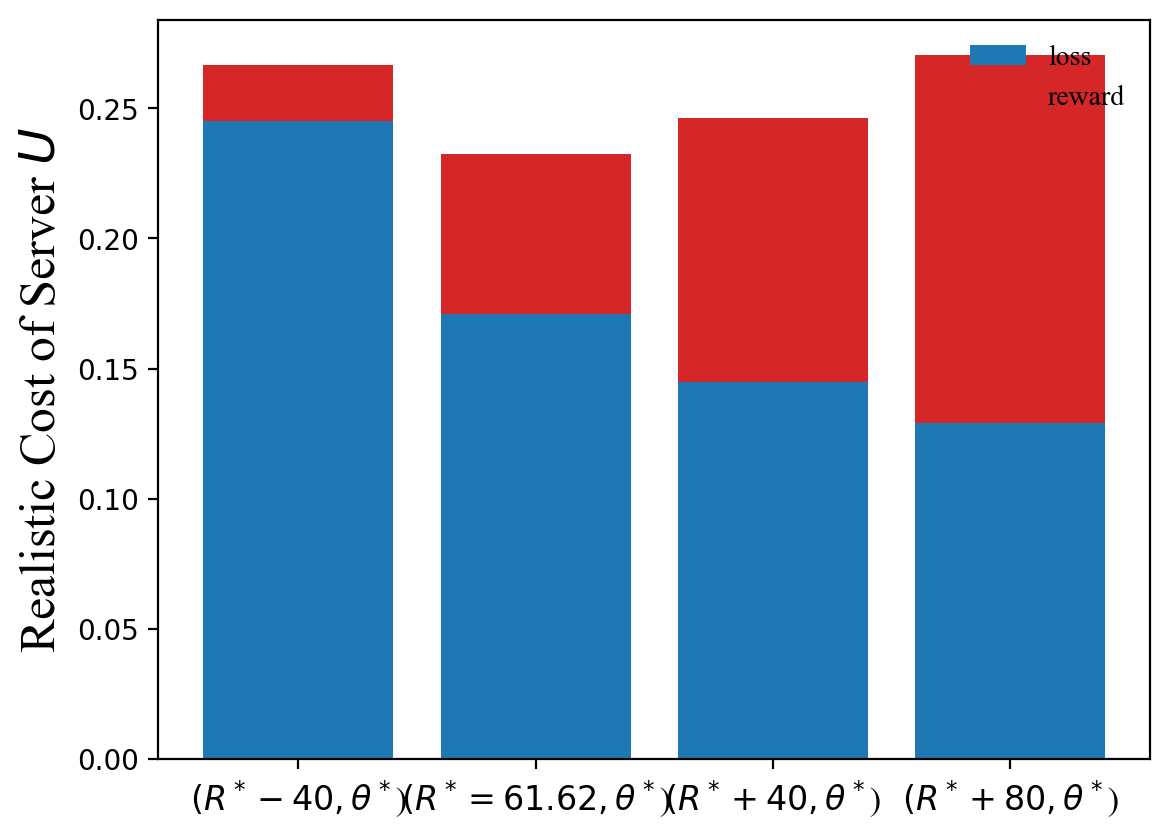
\includegraphics[width=\textwidth]{figures/figure_75_B.png}
    \caption{$\sigma=0.3$}
	\end{subfigure}
  \quad
  \begin{subfigure}{0.31\textwidth}
		\centering
		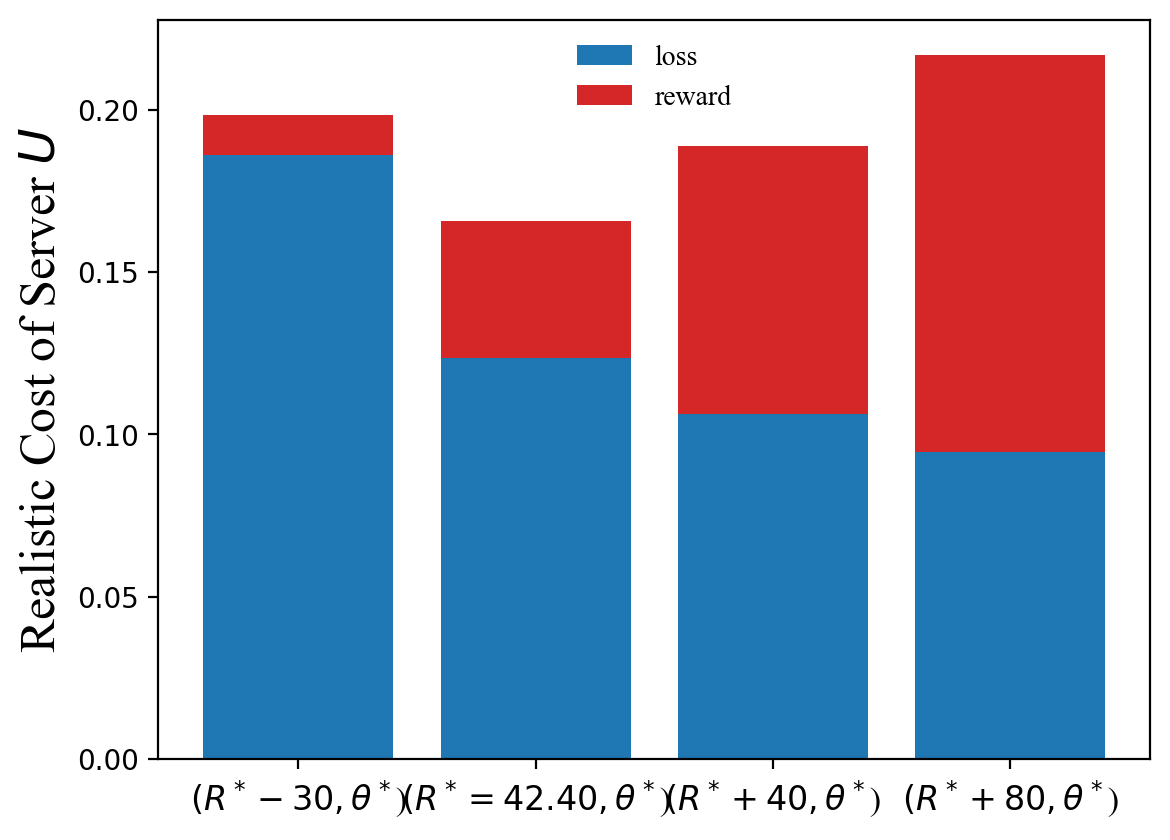
\includegraphics[width=\textwidth]{figures/figure_75_C.png}
    \caption{$\sigma=0.7$}
	\end{subfigure}
	\caption{The effect of $R$ on cost}
\end{figure}

\textit{Effect of initiative data on server' cost:}
\begin{figure}
	\begin{minipage}{0.32\linewidth}
		\vspace{3pt}
        %这个图片路径替换成你的图片路径即可使用
		\centerline{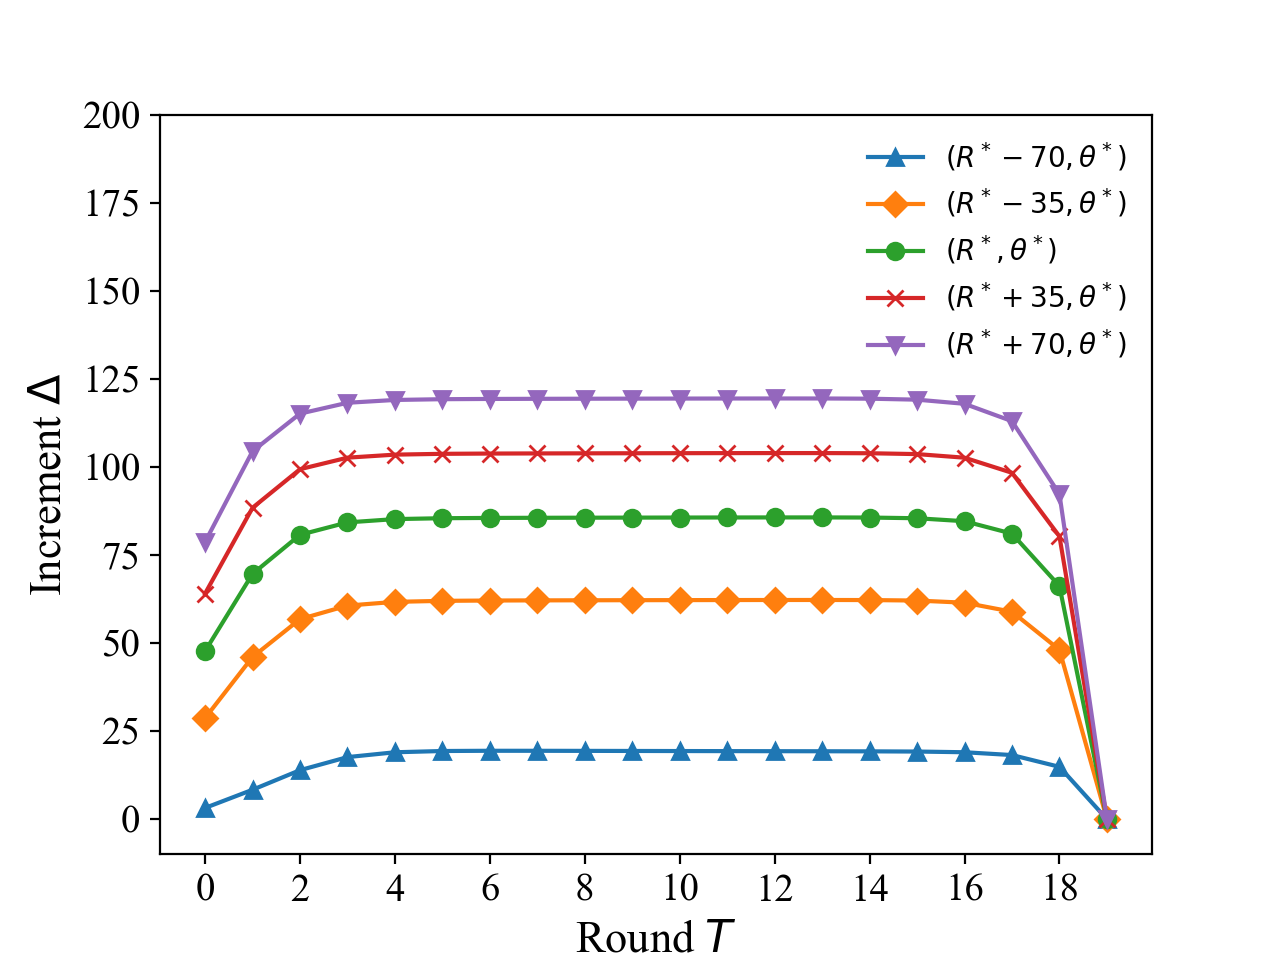
\includegraphics[width=\textwidth]{figures/figure_55_A.png}}
	\end{minipage}
	\begin{minipage}{0.32\linewidth}
		\vspace{3pt}
		\centerline{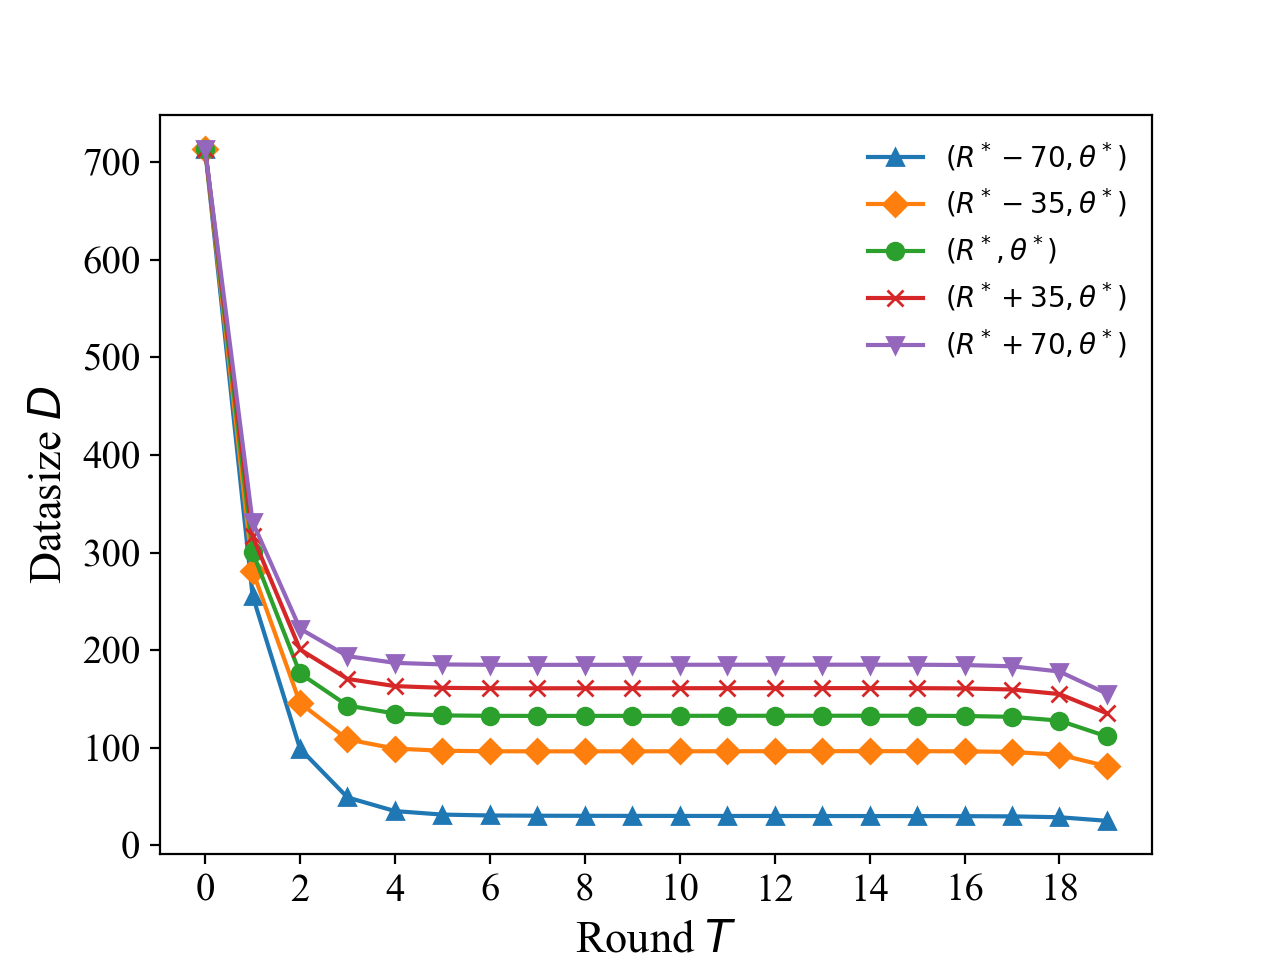
\includegraphics[width=\textwidth]{figures/figure_55_B.png}}
	\end{minipage}
  \begin{minipage}{0.32\linewidth}
		\vspace{3pt}
		\centerline{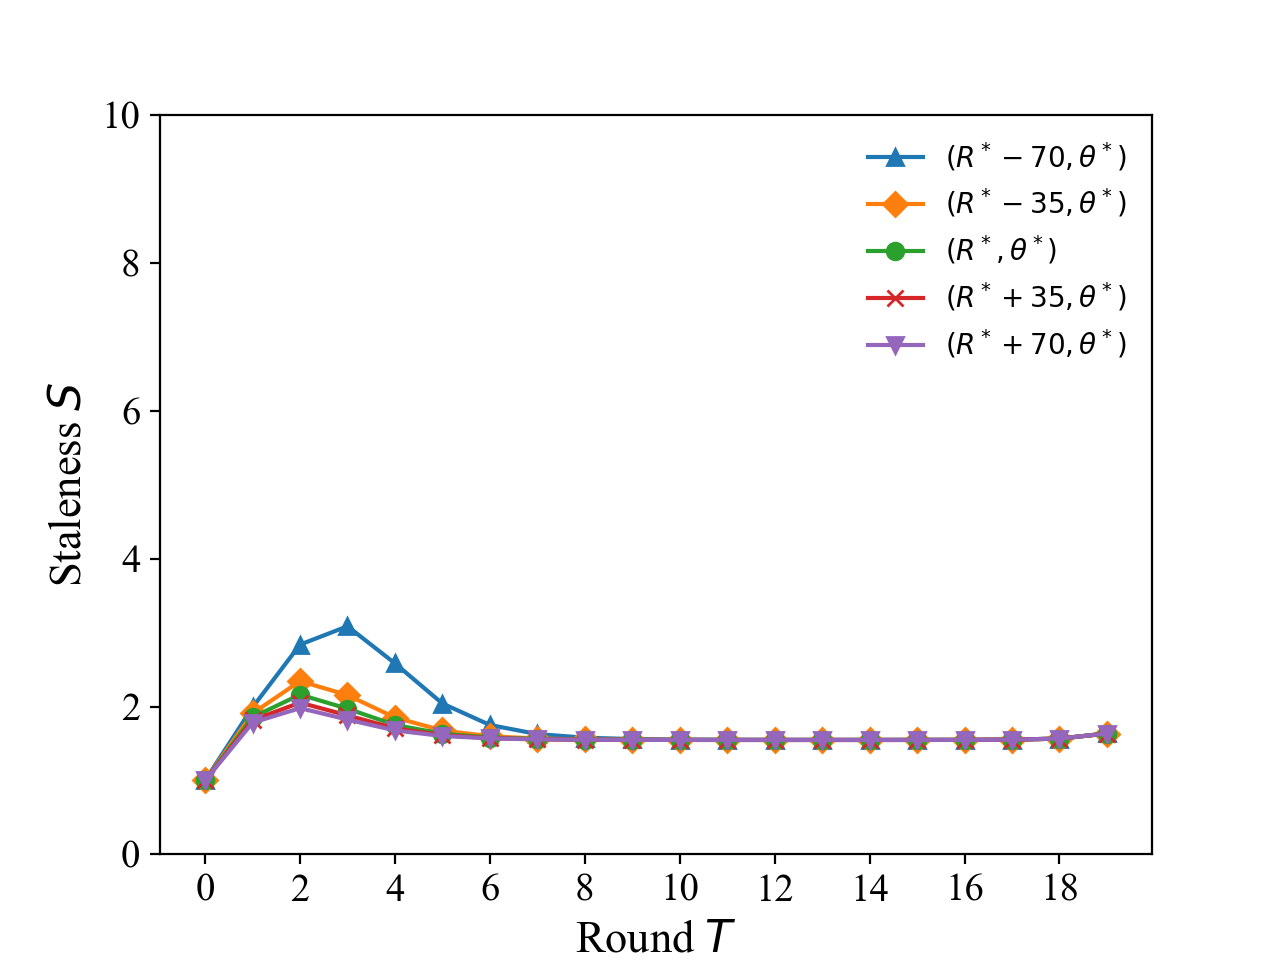
\includegraphics[width=\textwidth]{figures/figure_55_C.png}}
	\end{minipage}
  \qquad
	\begin{minipage}{0.32\linewidth}
		\vspace{3pt}
        %这个图片路径替换成你的图片路径即可使用
		\centerline{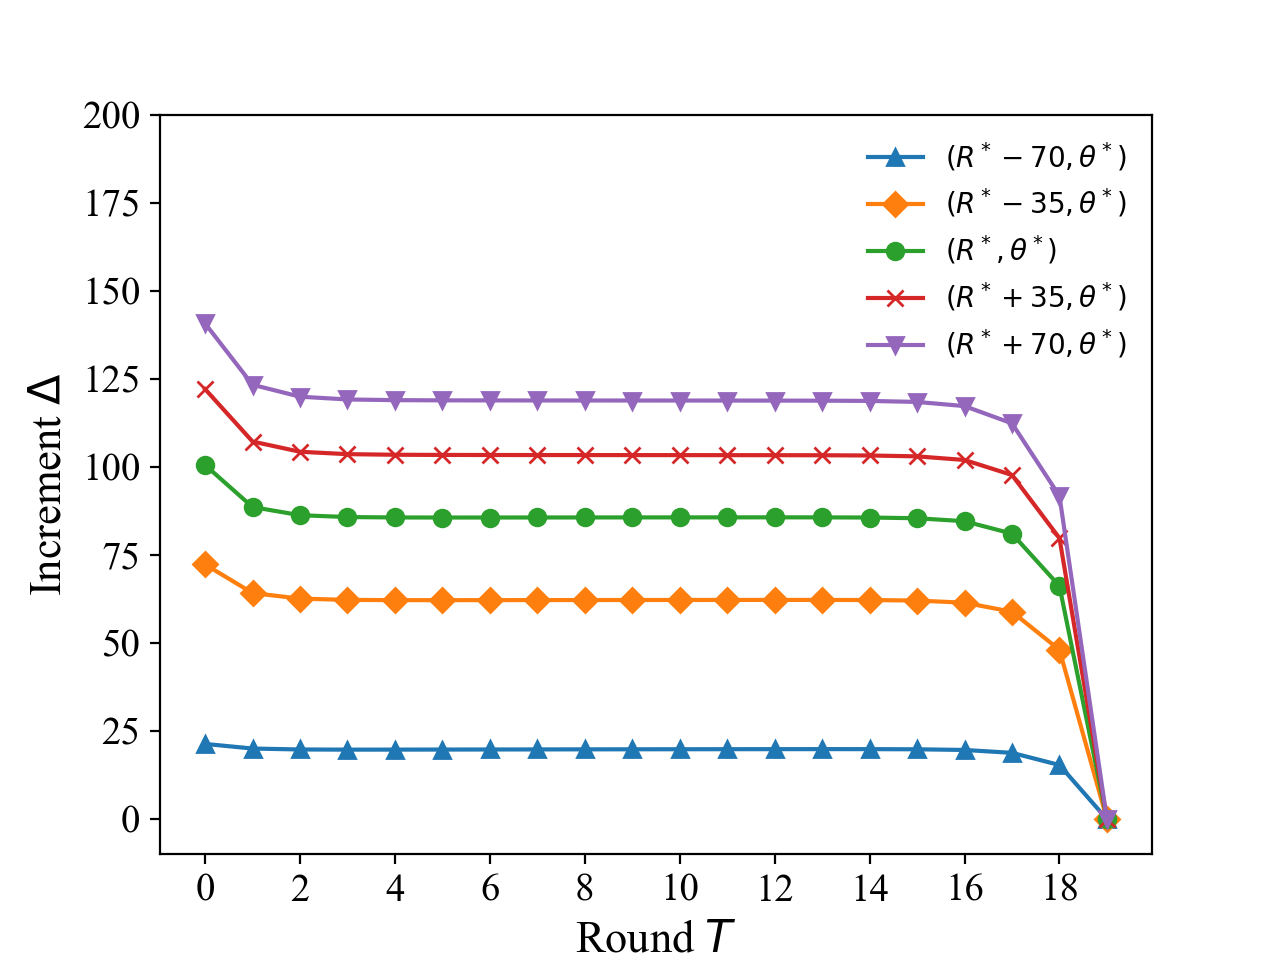
\includegraphics[width=\textwidth]{figures/figure_59_A.png}}
	\end{minipage}
	\begin{minipage}{0.32\linewidth}
		\vspace{3pt}
		\centerline{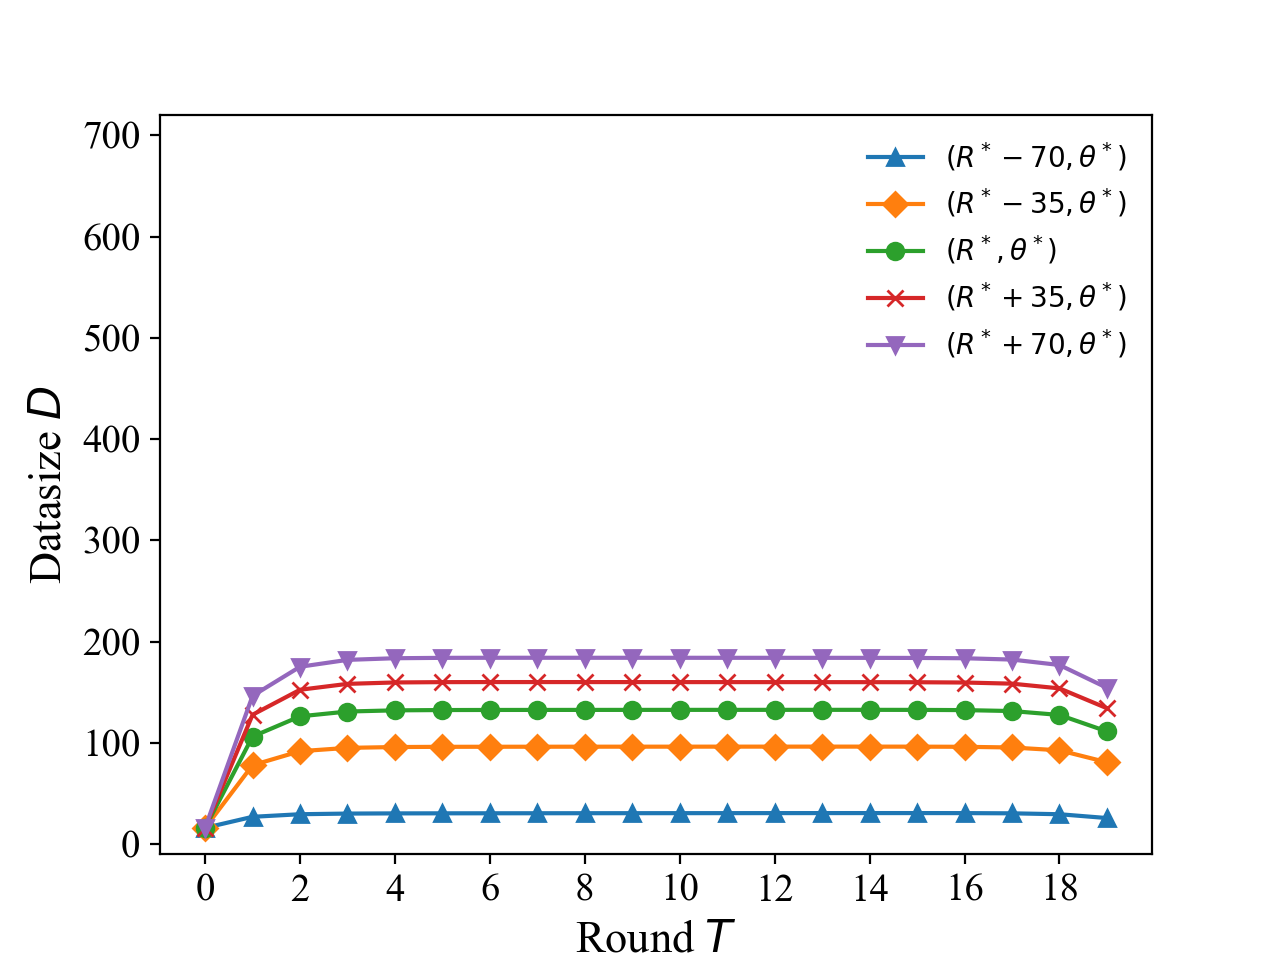
\includegraphics[width=\textwidth]{figures/figure_59_B.png}}
	\end{minipage}
  \begin{minipage}{0.32\linewidth}
		\vspace{3pt}
		\centerline{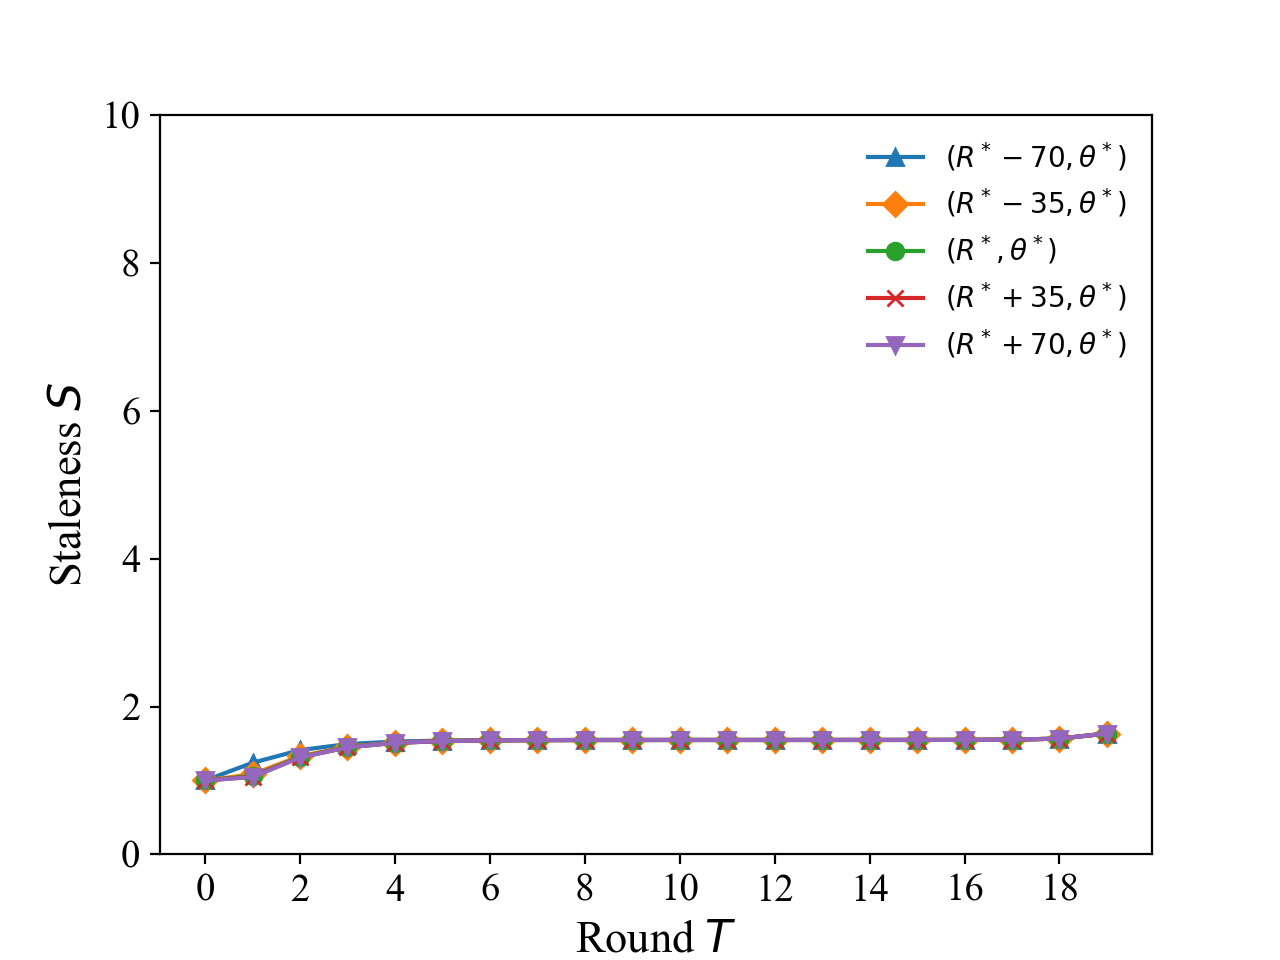
\includegraphics[width=\textwidth]{figures/figure_59_C.png}}
	\end{minipage}  
	\caption{The effect of $D_k(0)$ on data quality and quantity}
\end{figure}

\textit{Effect of initiative data on server' cost:}
\begin{figure}
	\begin{minipage}{0.32\linewidth}
		\vspace{3pt}
        %这个图片路径替换成你的图片路径即可使用
		\centerline{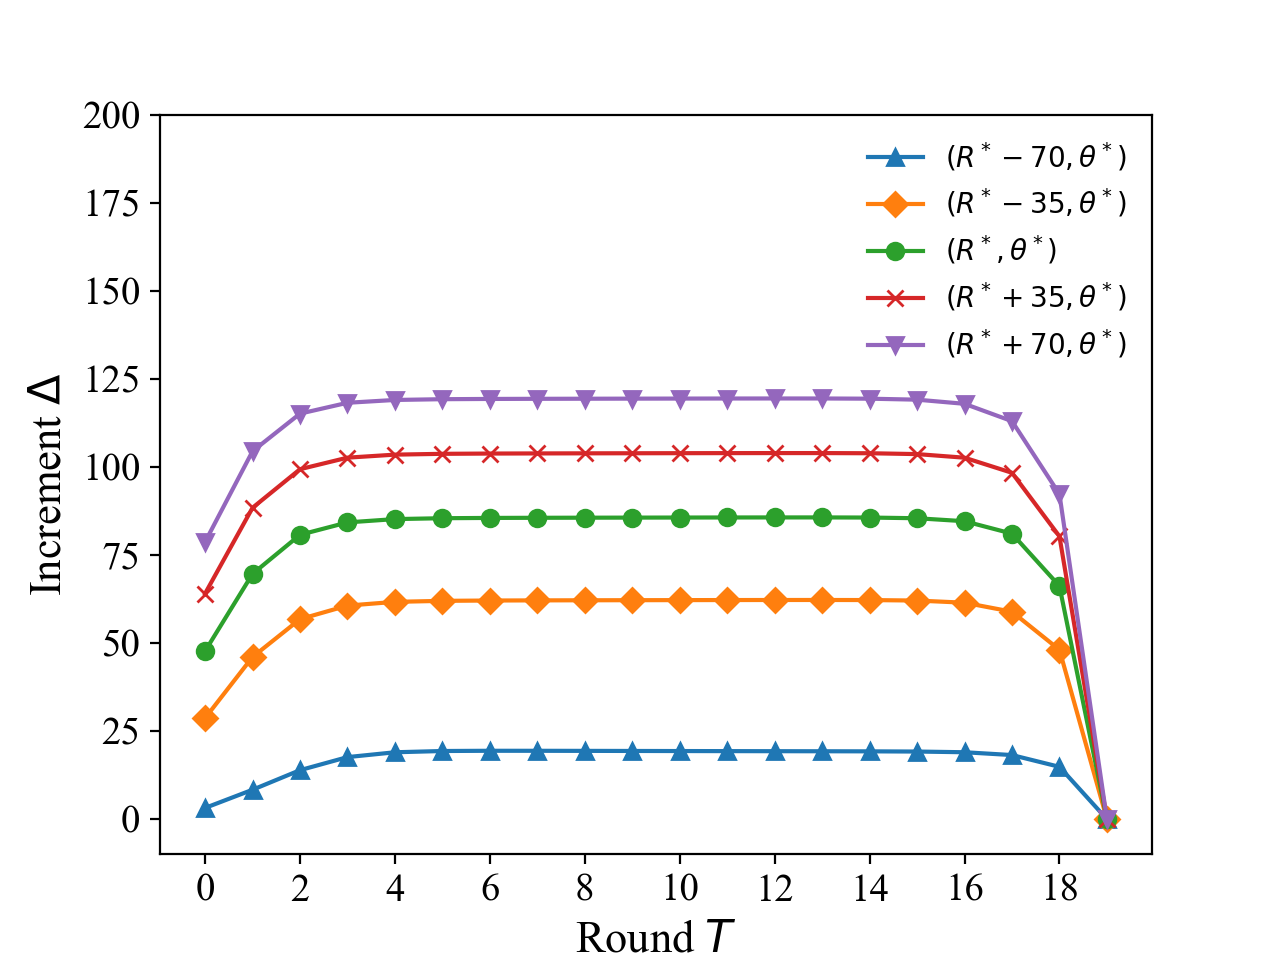
\includegraphics[width=\textwidth]{figures/figure_55_A.png}}
	\end{minipage}
	\begin{minipage}{0.32\linewidth}
		\vspace{3pt}
		\centerline{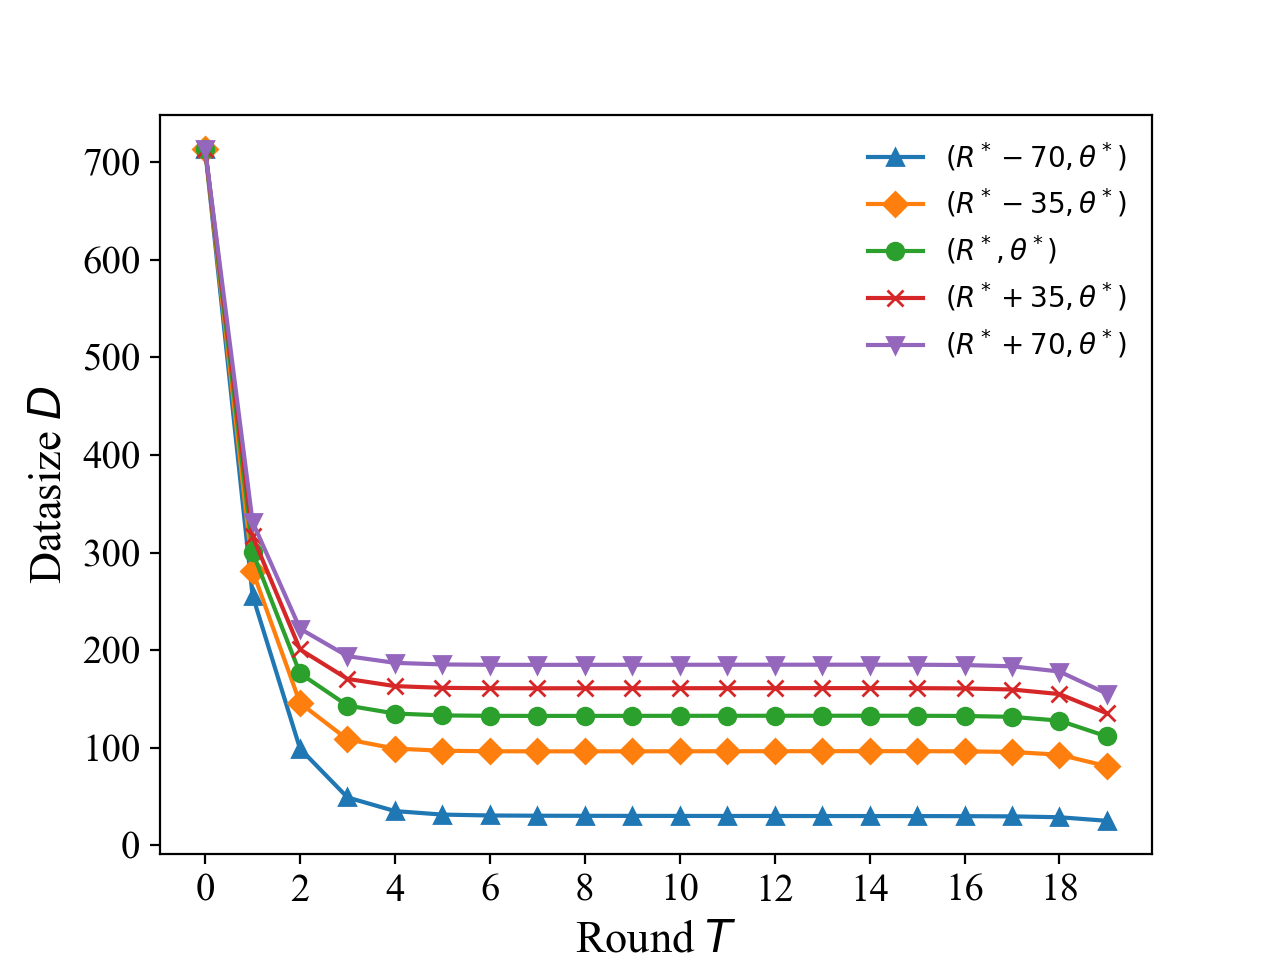
\includegraphics[width=\textwidth]{figures/figure_55_B.png}}
	\end{minipage}
  \begin{minipage}{0.32\linewidth}
		\vspace{3pt}
		\centerline{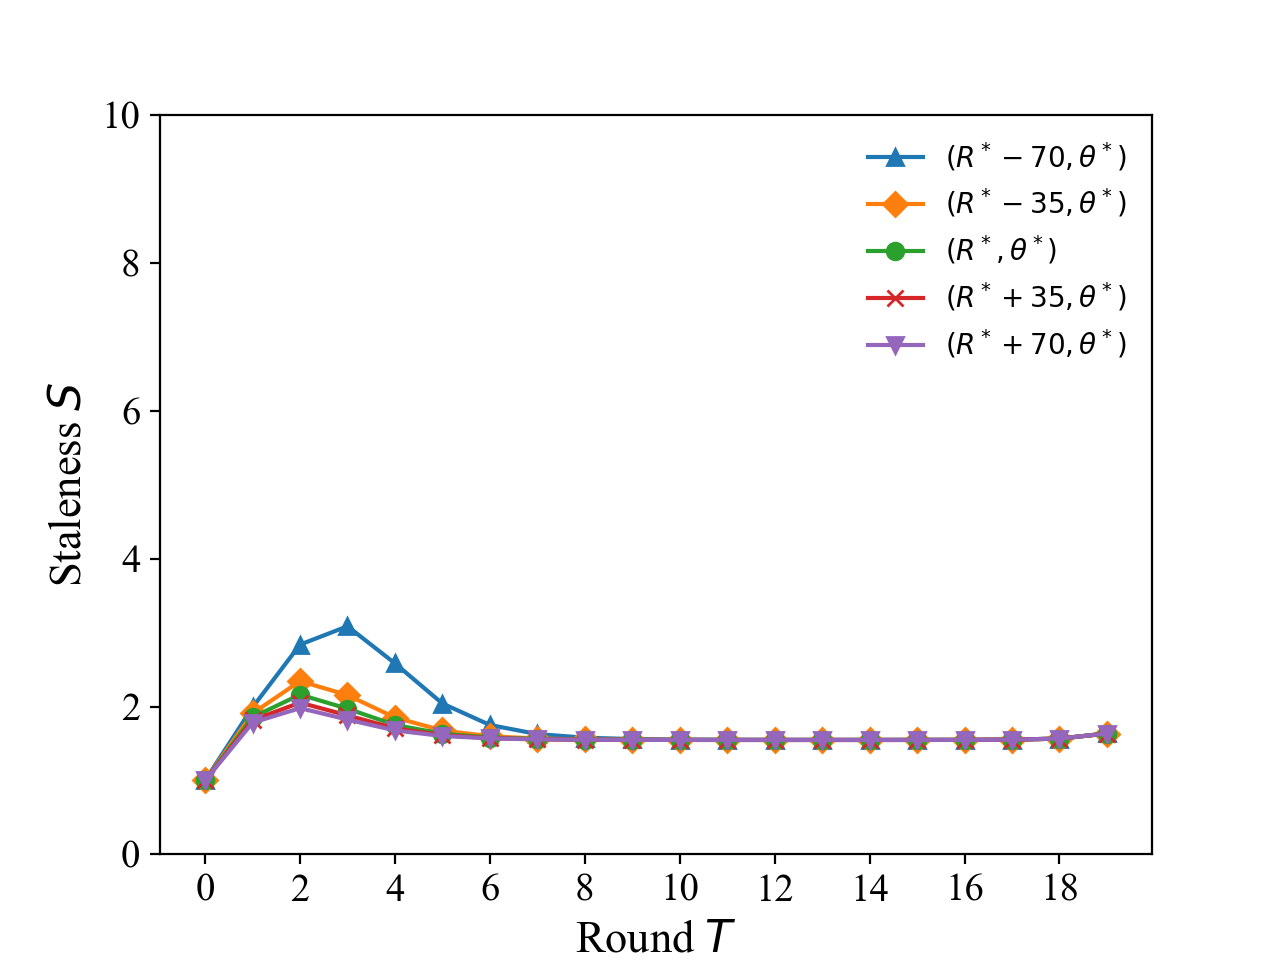
\includegraphics[width=\textwidth]{figures/figure_55_C.png}}
	\end{minipage}
  \qquad
	\begin{minipage}{0.33\linewidth}
		\vspace{3pt}
        %这个图片路径替换成你的图片路径即可使用
		\centerline{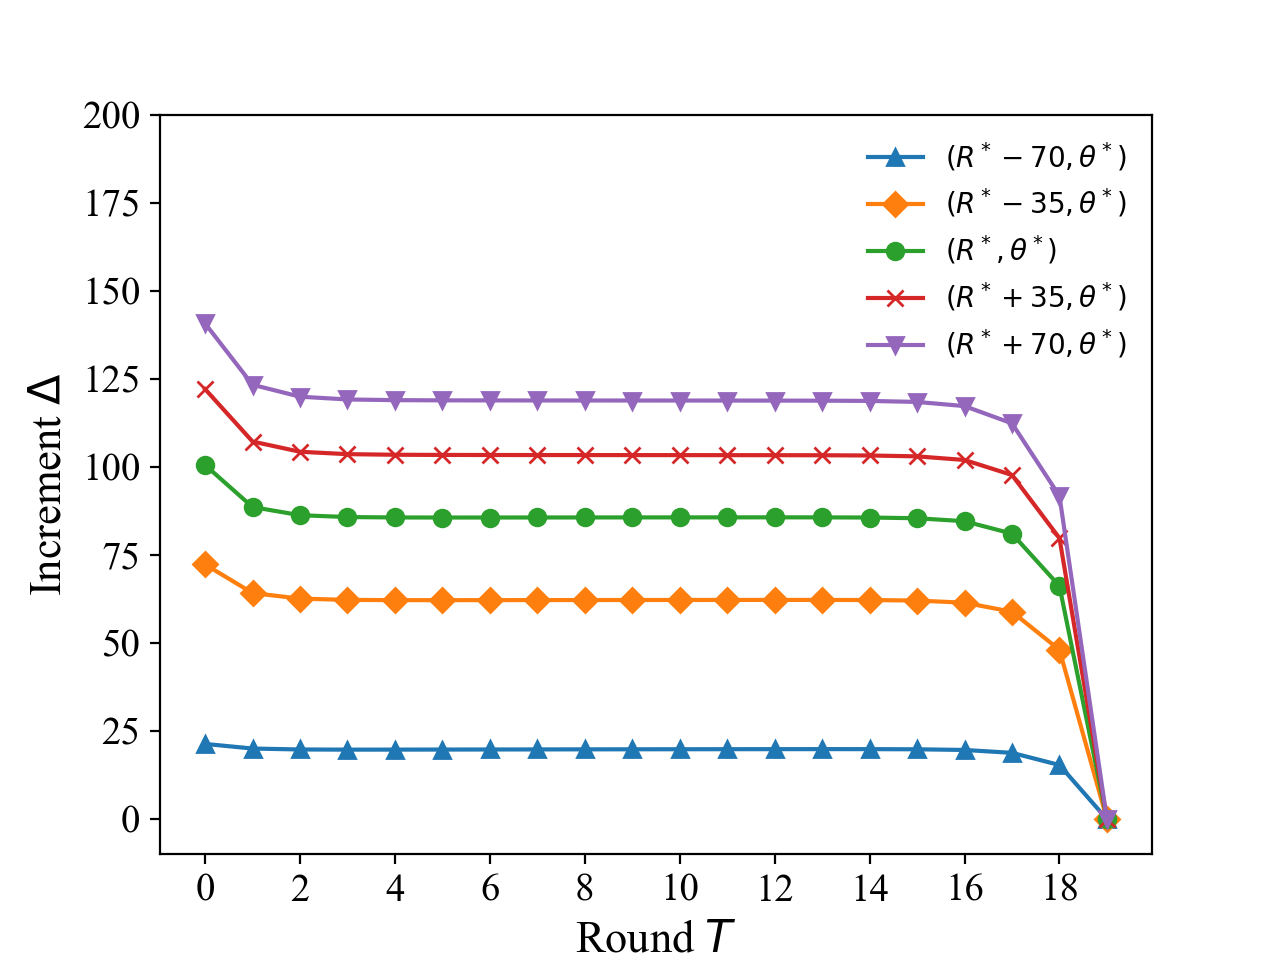
\includegraphics[width=\textwidth]{figures/figure_59_A.png}}
	\end{minipage}
	\begin{minipage}{0.33\linewidth}
		\vspace{3pt}
		\centerline{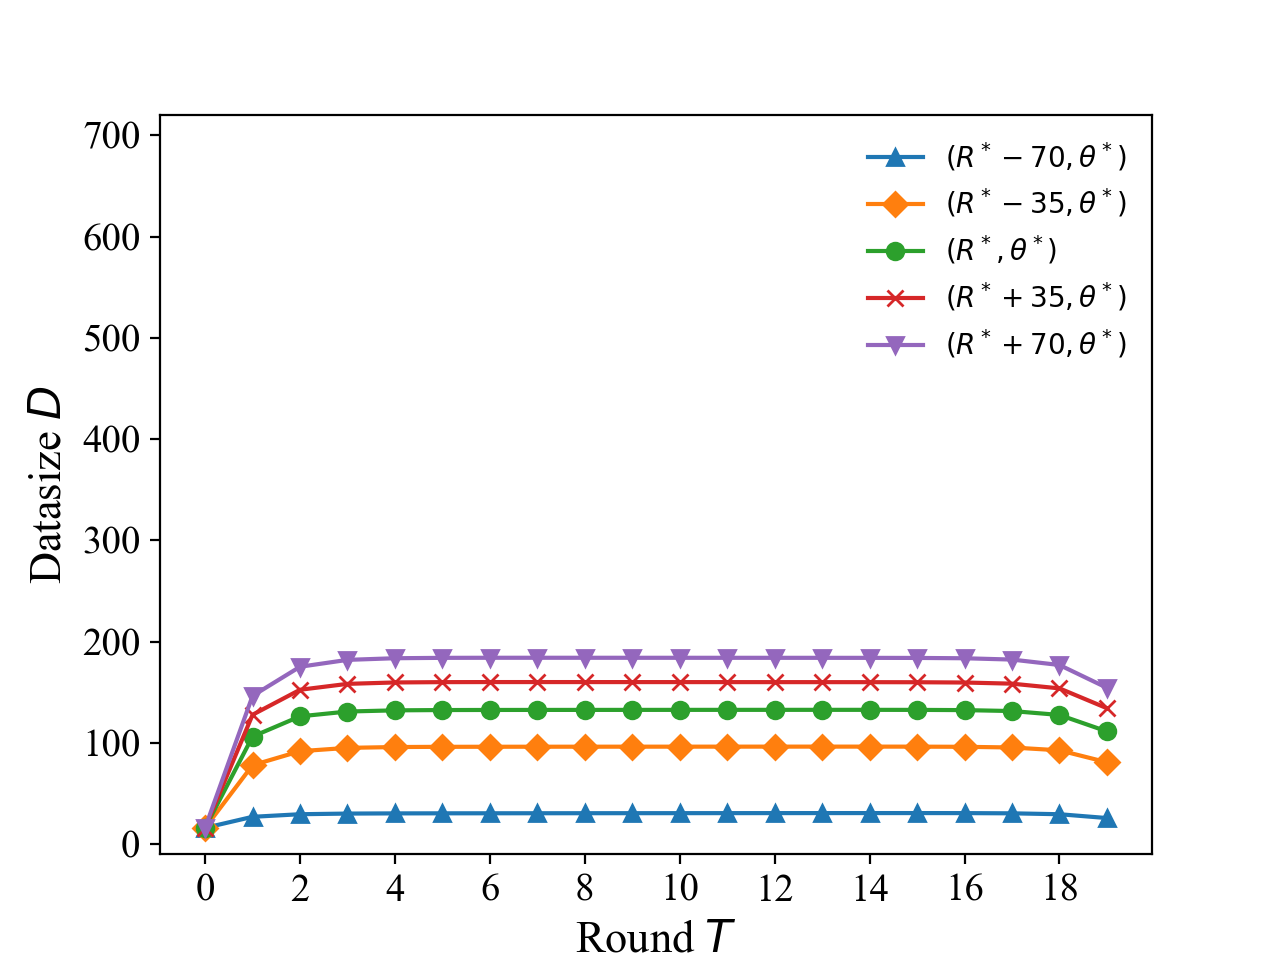
\includegraphics[width=\textwidth]{figures/figure_59_B.png}}
	\end{minipage}
  \begin{minipage}{0.33\linewidth}
		\vspace{3pt}
		\centerline{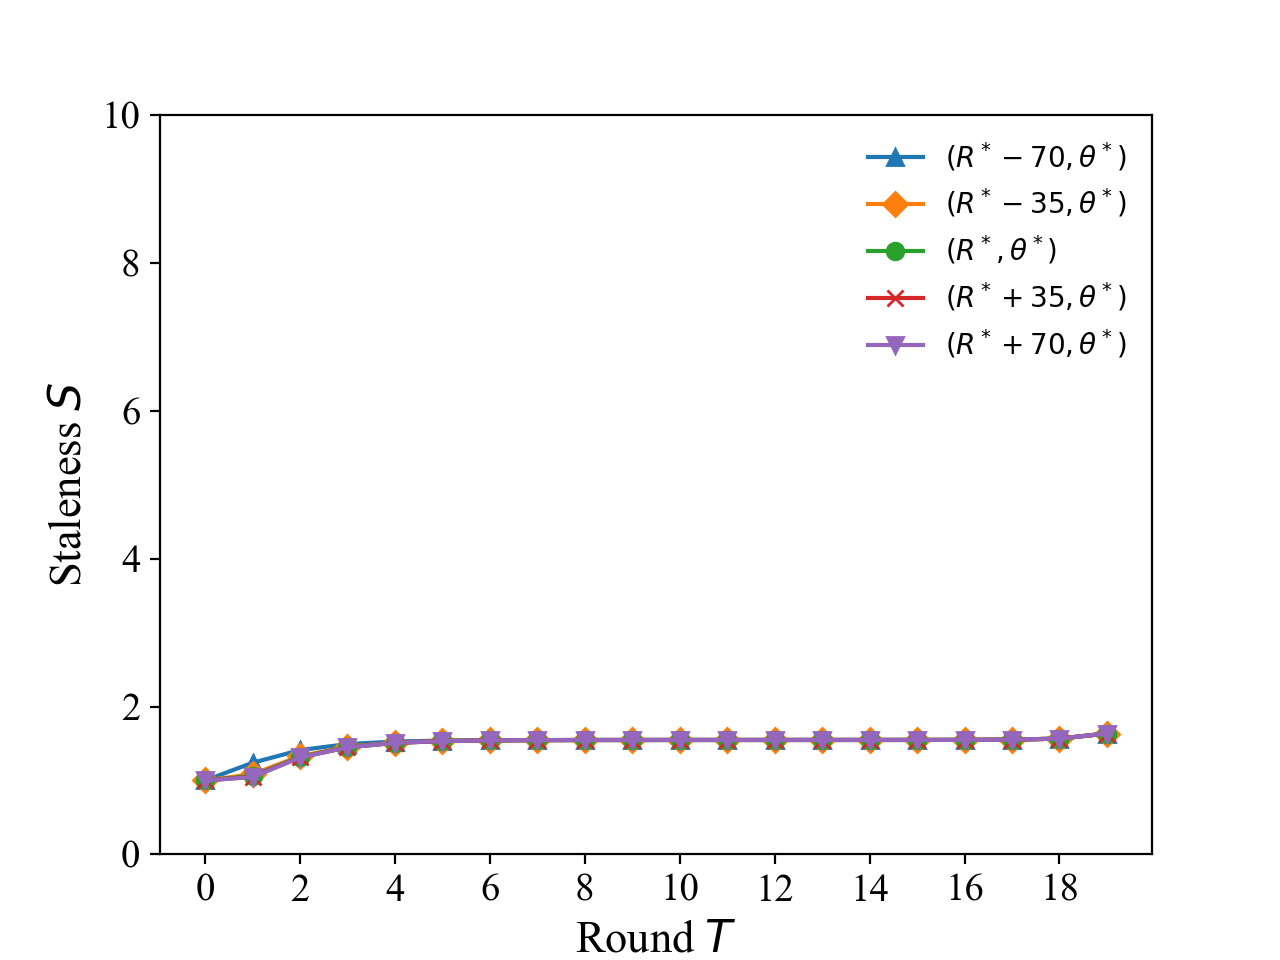
\includegraphics[width=\textwidth]{figures/figure_59_C.png}}
	\end{minipage}  
	\caption{The effect of $D_k(0)$ on data quality and quantity}
\end{figure}


\section{Electronic Submission}
\label{submission}

Submission to ICML 2025 will be entirely electronic, via a web site
(not email). Information about the submission process and \LaTeX\ templates
are available on the conference web site at:
\begin{center}
\textbf{\texttt{http://icml.cc/}}
\end{center}

The guidelines below will be enforced for initial submissions and
camera-ready copies. Here is a brief summary:
\begin{itemize}
\item Submissions must be in PDF\@. 
\item If your paper has appendices, submit the appendix together with the main body and the references \textbf{as a single file}. Reviewers will not look for appendices as a separate PDF file. So if you submit such an extra file, reviewers will very likely miss it.
\item Page limit: The main body of the paper has to be fitted to 8 pages, excluding references and appendices; the space for the latter two is not limited in pages, but the total file size may not exceed 10MB. For the final version of the paper, authors can add one extra page to the main body.
\item \textbf{Do not include author information or acknowledgements} in your
    initial submission.
\item Your paper should be in \textbf{10 point Times font}.
\item Make sure your PDF file only uses Type-1 fonts.
\item Place figure captions \emph{under} the figure (and omit titles from inside
    the graphic file itself). Place table captions \emph{over} the table.
\item References must include page numbers whenever possible and be as complete
    as possible. Place multiple citations in chronological order.
\item Do not alter the style template; in particular, do not compress the paper
    format by reducing the vertical spaces.
\item Keep your abstract brief and self-contained, one paragraph and roughly
    4--6 sentences. Gross violations will require correction at the
    camera-ready phase. The title should have content words capitalized.
\end{itemize}

\subsection{Submitting Papers}

\textbf{Anonymous Submission:} ICML uses double-blind review: no identifying
author information may appear on the title page or in the paper
itself. \cref{author info} gives further details.

\medskip

Authors must provide their manuscripts in \textbf{PDF} format.
Furthermore, please make sure that files contain only embedded Type-1 fonts
(e.g.,~using the program \texttt{pdffonts} in linux or using
File/DocumentProperties/Fonts in Acrobat). Other fonts (like Type-3)
might come from graphics files imported into the document.

Authors using \textbf{Word} must convert their document to PDF\@. Most
of the latest versions of Word have the facility to do this
automatically. Submissions will not be accepted in Word format or any
format other than PDF\@. Really. We're not joking. Don't send Word.

Those who use \textbf{\LaTeX} should avoid including Type-3 fonts.
Those using \texttt{latex} and \texttt{dvips} may need the following
two commands:

{\footnotesize
\begin{verbatim}
dvips -Ppdf -tletter -G0 -o paper.ps paper.dvi
ps2pdf paper.ps
\end{verbatim}}
It is a zero following the ``-G'', which tells dvips to use
the config.pdf file. Newer \TeX\ distributions don't always need this
option.

Using \texttt{pdflatex} rather than \texttt{latex}, often gives better
results. This program avoids the Type-3 font problem, and supports more
advanced features in the \texttt{microtype} package.

\textbf{Graphics files} should be a reasonable size, and included from
an appropriate format. Use vector formats (.eps/.pdf) for plots,
lossless bitmap formats (.png) for raster graphics with sharp lines, and
jpeg for photo-like images.

The style file uses the \texttt{hyperref} package to make clickable
links in documents. If this causes problems for you, add
\texttt{nohyperref} as one of the options to the \texttt{icml2025}
usepackage statement.


\subsection{Submitting Final Camera-Ready Copy}

The final versions of papers accepted for publication should follow the
same format and naming convention as initial submissions, except that
author information (names and affiliations) should be given. See
\cref{final author} for formatting instructions.

The footnote, ``Preliminary work. Under review by the International
Conference on Machine Learning (ICML). Do not distribute.'' must be
modified to ``\textit{Proceedings of the
$\mathit{42}^{nd}$ International Conference on Machine Learning},
Vancouver, Canada, PMLR 267, 2025.
Copyright 2025 by the author(s).''

For those using the \textbf{\LaTeX} style file, this change (and others) is
handled automatically by simply changing
$\mathtt{\backslash usepackage\{icml2025\}}$ to
$$\mathtt{\backslash usepackage[accepted]\{icml2025\}}$$
Authors using \textbf{Word} must edit the
footnote on the first page of the document themselves.

Camera-ready copies should have the title of the paper as running head
on each page except the first one. The running title consists of a
single line centered above a horizontal rule which is $1$~point thick.
The running head should be centered, bold and in $9$~point type. The
rule should be $10$~points above the main text. For those using the
\textbf{\LaTeX} style file, the original title is automatically set as running
head using the \texttt{fancyhdr} package which is included in the ICML
2025 style file package. In case that the original title exceeds the
size restrictions, a shorter form can be supplied by using

\verb|\icmltitlerunning{...}|

just before $\mathtt{\backslash begin\{document\}}$.
Authors using \textbf{Word} must edit the header of the document themselves.





\section{Format of the Paper}

All submissions must follow the specified format.

\subsection{Dimensions}




The text of the paper should be formatted in two columns, with an
overall width of 6.75~inches, height of 9.0~inches, and 0.25~inches
between the columns. The left margin should be 0.75~inches and the top
margin 1.0~inch (2.54~cm). The right and bottom margins will depend on
whether you print on US letter or A4 paper, but all final versions
must be produced for US letter size.
Do not write anything on the margins.

The paper body should be set in 10~point type with a vertical spacing
of 11~points. Please use Times typeface throughout the text.

\subsection{Title}

The paper title should be set in 14~point bold type and centered
between two horizontal rules that are 1~point thick, with 1.0~inch
between the top rule and the top edge of the page. Capitalize the
first letter of content words and put the rest of the title in lower
case.

\subsection{Author Information for Submission}
\label{author info}

ICML uses double-blind review, so author information must not appear. If
you are using \LaTeX\/ and the \texttt{icml2025.sty} file, use
\verb+\icmlauthor{...}+ to specify authors and \verb+\icmlaffiliation{...}+ to specify affiliations. (Read the TeX code used to produce this document for an example usage.) The author information
will not be printed unless \texttt{accepted} is passed as an argument to the
style file.
Submissions that include the author information will not
be reviewed.

\subsubsection{Self-Citations}

If you are citing published papers for which you are an author, refer
to yourself in the third person. In particular, do not use phrases
that reveal your identity (e.g., ``in previous work \cite{langley00}, we
have shown \ldots'').

Do not anonymize citations in the reference section. The only exception are manuscripts that are
not yet published (e.g., under submission). If you choose to refer to
such unpublished manuscripts \cite{anonymous}, anonymized copies have
to be submitted
as Supplementary Material via OpenReview\@. However, keep in mind that an ICML
paper should be self contained and should contain sufficient detail
for the reviewers to evaluate the work. In particular, reviewers are
not required to look at the Supplementary Material when writing their
review (they are not required to look at more than the first $8$ pages of the submitted document).

\subsubsection{Camera-Ready Author Information}
\label{final author}

If a paper is accepted, a final camera-ready copy must be prepared.
%
For camera-ready papers, author information should start 0.3~inches below the
bottom rule surrounding the title. The authors' names should appear in 10~point
bold type, in a row, separated by white space, and centered. Author names should
not be broken across lines. Unbolded superscripted numbers, starting 1, should
be used to refer to affiliations.

Affiliations should be numbered in the order of appearance. A single footnote
block of text should be used to list all the affiliations. (Academic
affiliations should list Department, University, City, State/Region, Country.
Similarly for industrial affiliations.)

Each distinct affiliations should be listed once. If an author has multiple
affiliations, multiple superscripts should be placed after the name, separated
by thin spaces. If the authors would like to highlight equal contribution by
multiple first authors, those authors should have an asterisk placed after their
name in superscript, and the term ``\textsuperscript{*}Equal contribution"
should be placed in the footnote block ahead of the list of affiliations. A
list of corresponding authors and their emails (in the format Full Name
\textless{}email@domain.com\textgreater{}) can follow the list of affiliations.
Ideally only one or two names should be listed.

A sample file with author names is included in the ICML2025 style file
package. Turn on the \texttt{[accepted]} option to the stylefile to
see the names rendered. All of the guidelines above are implemented
by the \LaTeX\ style file.

\subsection{Abstract}

The paper abstract should begin in the left column, 0.4~inches below the final
address. The heading `Abstract' should be centered, bold, and in 11~point type.
The abstract body should use 10~point type, with a vertical spacing of
11~points, and should be indented 0.25~inches more than normal on left-hand and
right-hand margins. Insert 0.4~inches of blank space after the body. Keep your
abstract brief and self-contained, limiting it to one paragraph and roughly 4--6
sentences. Gross violations will require correction at the camera-ready phase.

\subsection{Partitioning the Text}

You should organize your paper into sections and paragraphs to help
readers place a structure on the material and understand its
contributions.

\subsubsection{Sections and Subsections}

Section headings should be numbered, flush left, and set in 11~pt bold
type with the content words capitalized. Leave 0.25~inches of space
before the heading and 0.15~inches after the heading.

Similarly, subsection headings should be numbered, flush left, and set
in 10~pt bold type with the content words capitalized. Leave
0.2~inches of space before the heading and 0.13~inches afterward.

Finally, subsubsection headings should be numbered, flush left, and
set in 10~pt small caps with the content words capitalized. Leave
0.18~inches of space before the heading and 0.1~inches after the
heading.

Please use no more than three levels of headings.

\subsubsection{Paragraphs and Footnotes}

Within each section or subsection, you should further partition the
paper into paragraphs. Do not indent the first line of a given
paragraph, but insert a blank line between succeeding ones.

You can use footnotes\footnote{Footnotes
should be complete sentences.} to provide readers with additional
information about a topic without interrupting the flow of the paper.
Indicate footnotes with a number in the text where the point is most
relevant. Place the footnote in 9~point type at the bottom of the
column in which it appears. Precede the first footnote in a column
with a horizontal rule of 0.8~inches.\footnote{Multiple footnotes can
appear in each column, in the same order as they appear in the text,
but spread them across columns and pages if possible.}

\begin{figure}[ht]
\vskip 0.2in
\begin{center}
\centerline{\includegraphics[width=\columnwidth]{icml_numpapers}}
\caption{Historical locations and number of accepted papers for International
Machine Learning Conferences (ICML 1993 -- ICML 2008) and International
Workshops on Machine Learning (ML 1988 -- ML 1992). At the time this figure was
produced, the number of accepted papers for ICML 2008 was unknown and instead
estimated.}
\label{icml-historical}
\end{center}
\vskip -0.2in
\end{figure}

\subsection{Figures}

You may want to include figures in the paper to illustrate
your approach and results. Such artwork should be centered,
legible, and separated from the text. Lines should be dark and at
least 0.5~points thick for purposes of reproduction, and text should
not appear on a gray background.

Label all distinct components of each figure. If the figure takes the
form of a graph, then give a name for each axis and include a legend
that briefly describes each curve. Do not include a title inside the
figure; instead, the caption should serve this function.

Number figures sequentially, placing the figure number and caption
\emph{after} the graphics, with at least 0.1~inches of space before
the caption and 0.1~inches after it, as in
\cref{icml-historical}. The figure caption should be set in
9~point type and centered unless it runs two or more lines, in which
case it should be flush left. You may float figures to the top or
bottom of a column, and you may set wide figures across both columns
(use the environment \texttt{figure*} in \LaTeX). Always place
two-column figures at the top or bottom of the page.

\subsection{Algorithms}

If you are using \LaTeX, please use the ``algorithm'' and ``algorithmic''
environments to format pseudocode. These require
the corresponding stylefiles, algorithm.sty and
algorithmic.sty, which are supplied with this package.
\cref{alg:example} shows an example.

\begin{algorithm}[tb]
   \caption{Bubble Sort}
   \label{alg:example}
\begin{algorithmic}
   \STATE {\bfseries Input:} data $x_i$, size $m$
   \REPEAT
   \STATE Initialize $noChange = true$.
   \FOR{$i=1$ {\bfseries to} $m-1$}
   \IF{$x_i > x_{i+1}$}
   \STATE Swap $x_i$ and $x_{i+1}$
   \STATE $noChange = false$
   \ENDIF
   \ENDFOR
   \UNTIL{$noChange$ is $true$}
\end{algorithmic}
\end{algorithm}

\subsection{Tables}

You may also want to include tables that summarize material. Like
figures, these should be centered, legible, and numbered consecutively.
However, place the title \emph{above} the table with at least
0.1~inches of space before the title and the same after it, as in
\cref{sample-table}. The table title should be set in 9~point
type and centered unless it runs two or more lines, in which case it
should be flush left.

% Note use of \abovespace and \belowspace to get reasonable spacing
% above and below tabular lines.

\begin{table}[t]
\caption{Classification accuracies for naive Bayes and flexible
Bayes on various data sets.}
\label{sample-table}
\vskip 0.15in
\begin{center}
\begin{small}
\begin{sc}
\begin{tabular}{lcccr}
\toprule
Data set & Naive & Flexible & Better? \\
\midrule
Breast    & 95.9$\pm$ 0.2& 96.7$\pm$ 0.2& $\surd$ \\
Cleveland & 83.3$\pm$ 0.6& 80.0$\pm$ 0.6& $\times$\\
Glass2    & 61.9$\pm$ 1.4& 83.8$\pm$ 0.7& $\surd$ \\
Credit    & 74.8$\pm$ 0.5& 78.3$\pm$ 0.6&         \\
Horse     & 73.3$\pm$ 0.9& 69.7$\pm$ 1.0& $\times$\\
Meta      & 67.1$\pm$ 0.6& 76.5$\pm$ 0.5& $\surd$ \\
Pima      & 75.1$\pm$ 0.6& 73.9$\pm$ 0.5&         \\
Vehicle   & 44.9$\pm$ 0.6& 61.5$\pm$ 0.4& $\surd$ \\
\bottomrule
\end{tabular}
\end{sc}
\end{small}
\end{center}
\vskip -0.1in
\end{table}

Tables contain textual material, whereas figures contain graphical material.
Specify the contents of each row and column in the table's topmost
row. Again, you may float tables to a column's top or bottom, and set
wide tables across both columns. Place two-column tables at the
top or bottom of the page.

\subsection{Theorems and such}
The preferred way is to number definitions, propositions, lemmas, etc. consecutively, within sections, as shown below.
\begin{definition}
\label{def:inj}
A function $f:X \to Y$ is injective if for any $x,y\in X$ different, $f(x)\ne f(y)$.
\end{definition}
Using \cref{def:inj} we immediate get the following result:
\begin{proposition}
If $f$ is injective mapping a set $X$ to another set $Y$, 
the cardinality of $Y$ is at least as large as that of $X$
\end{proposition}
\begin{proof} 
Left as an exercise to the reader. 
\end{proof}
\cref{lem:usefullemma} stated next will prove to be useful.
\begin{lemma}
\label{lem:usefullemma}
For any $f:X \to Y$ and $g:Y\to Z$ injective functions, $f \circ g$ is injective.
\end{lemma}
\begin{theorem}
\label{thm:bigtheorem}
If $f:X\to Y$ is bijective, the cardinality of $X$ and $Y$ are the same.
\end{theorem}
An easy corollary of \cref{thm:bigtheorem} is the following:
\begin{corollary}
If $f:X\to Y$ is bijective, 
the cardinality of $X$ is at least as large as that of $Y$.
\end{corollary}
\begin{assumption}
The set $X$ is finite.
\label{ass:xfinite}
\end{assumption}
\begin{remark}
According to some, it is only the finite case (cf. \cref{ass:xfinite}) that is interesting.
\end{remark}
%restatable

\subsection{Citations and References}

Please use APA reference format regardless of your formatter
or word processor. If you rely on the \LaTeX\/ bibliographic
facility, use \texttt{natbib.sty} and \texttt{icml2025.bst}
included in the style-file package to obtain this format.

Citations within the text should include the authors' last names and
year. If the authors' names are included in the sentence, place only
the year in parentheses, for example when referencing Arthur Samuel's
pioneering work \yrcite{Samuel59}. Otherwise place the entire
reference in parentheses with the authors and year separated by a
comma \cite{Samuel59}. List multiple references separated by
semicolons \cite{kearns89,Samuel59,mitchell80}. Use the `et~al.'
construct only for citations with three or more authors or after
listing all authors to a publication in an earlier reference \cite{MachineLearningI}.

Authors should cite their own work in the third person
in the initial version of their paper submitted for blind review.
Please refer to \cref{author info} for detailed instructions on how to
cite your own papers.

Use an unnumbered first-level section heading for the references, and use a
hanging indent style, with the first line of the reference flush against the
left margin and subsequent lines indented by 10 points. The references at the
end of this document give examples for journal articles \cite{Samuel59},
conference publications \cite{langley00}, book chapters \cite{Newell81}, books
\cite{DudaHart2nd}, edited volumes \cite{MachineLearningI}, technical reports
\cite{mitchell80}, and dissertations \cite{kearns89}.

Alphabetize references by the surnames of the first authors, with
single author entries preceding multiple author entries. Order
references for the same authors by year of publication, with the
earliest first. Make sure that each reference includes all relevant
information (e.g., page numbers).

Please put some effort into making references complete, presentable, and
consistent, e.g. use the actual current name of authors.
If using bibtex, please protect capital letters of names and
abbreviations in titles, for example, use \{B\}ayesian or \{L\}ipschitz
in your .bib file.

\section*{Accessibility}
Authors are kindly asked to make their submissions as accessible as possible for everyone including people with disabilities and sensory or neurological differences.
Tips of how to achieve this and what to pay attention to will be provided on the conference website \url{http://icml.cc/}.

\section*{Software and Data}

If a paper is accepted, we strongly encourage the publication of software and data with the
camera-ready version of the paper whenever appropriate. This can be
done by including a URL in the camera-ready copy. However, \textbf{do not}
include URLs that reveal your institution or identity in your
submission for review. Instead, provide an anonymous URL or upload
the material as ``Supplementary Material'' into the OpenReview reviewing
system. Note that reviewers are not required to look at this material
when writing their review.

% Acknowledgements should only appear in the accepted version.
\section*{Acknowledgements}

\textbf{Do not} include acknowledgements in the initial version of
the paper submitted for blind review.

If a paper is accepted, the final camera-ready version can (and
usually should) include acknowledgements.  Such acknowledgements
should be placed at the end of the section, in an unnumbered section
that does not count towards the paper page limit. Typically, this will 
include thanks to reviewers who gave useful comments, to colleagues 
who contributed to the ideas, and to funding agencies and corporate 
sponsors that provided financial support.

\section*{Impact Statement}

Authors are \textbf{required} to include a statement of the potential 
broader impact of their work, including its ethical aspects and future 
societal consequences. This statement should be in an unnumbered 
section at the end of the paper (co-located with Acknowledgements -- 
the two may appear in either order, but both must be before References), 
and does not count toward the paper page limit. In many cases, where 
the ethical impacts and expected societal implications are those that 
are well established when advancing the field of Machine Learning, 
substantial discussion is not required, and a simple statement such 
as the following will suffice:

``This paper presents work whose goal is to advance the field of 
Machine Learning. There are many potential societal consequences 
of our work, none which we feel must be specifically highlighted here.''

The above statement can be used verbatim in such cases, but we 
encourage authors to think about whether there is content which does 
warrant further discussion, as this statement will be apparent if the 
paper is later flagged for ethics review.


% In the unusual situation where you want a paper to appear in the
% references without citing it in the main text, use \nocite
\nocite{langley00}

\bibliography{example_paper}
\bibliographystyle{icml2025}


%%%%%%%%%%%%%%%%%%%%%%%%%%%%%%%%%%%%%%%%%%%%%%%%%%%%%%%%%%%%%%%%%%%%%%%%%%%%%%%
%%%%%%%%%%%%%%%%%%%%%%%%%%%%%%%%%%%%%%%%%%%%%%%%%%%%%%%%%%%%%%%%%%%%%%%%%%%%%%%
% APPENDIX
%%%%%%%%%%%%%%%%%%%%%%%%%%%%%%%%%%%%%%%%%%%%%%%%%%%%%%%%%%%%%%%%%%%%%%%%%%%%%%%
%%%%%%%%%%%%%%%%%%%%%%%%%%%%%%%%%%%%%%%%%%%%%%%%%%%%%%%%%%%%%%%%%%%%%%%%%%%%%%%
\newpage
\appendix
\onecolumn
In the appendix, the complete proofs of theoretic results provided in the main text and more contents about experiment will be exhibited in detail.
\section{Proof of Theoretic Results}
\subsection{Proof of Collary 3.2}
\begin{proof}
    According to the definition of DoS, we have
    \begin{align}
      S_k(t+1) & = S_k(t) \frac{\theta D_k(t)}{D_k(t+1)} + 1 = S_k(t)\left(1 - \frac{\Delta_k(t)}{D_k(t+1)}\right) + 1 \notag \\
               & = \left(S_k(t-1) \frac{\theta D_k(t-1)}{D_k(t)} + 1\right) \frac{\theta D_k(t)}{D_k(t+1)} + 1 \notag \\
               & = S_k(t-1) \frac{\theta^2 D_k(t-1)}{D_k(t+1)} + \frac{\theta D_k(t)}{D_k(t+1)} + 1 \notag \\
               & = S_k(t-2) \frac{\theta^3 D_k(t-2)}{D_k(t+1)} + \frac{\theta^2 D_k(t-1)}{D_k(t+1)} + \frac{\theta D_k(t)}{D_k(t+1)} + 1 \notag \\
               & = \cdots \notag \\
               & = S_k(0) \frac{\theta^{t+1} D_k(0)}{D_k(t+1)} + \frac{\theta^t D_k(1)}{D_k(t+1)} + \cdots + \frac{\theta^2 D_k(t-1)}{D_k(t+1)} + \frac{\theta D_k(t)}{D_k(t+1)} + 1 \notag \\
               & = \sum_{\tau = 0}^{t+1} \frac{\theta^{t+1-\tau} D_k(\tau)}{D_k(t+1)}.
    \end{align}
  \end{proof}

\subsection{Proof of Theorem 3.10}
\begin{proof}
  Let's pay attention to the round $t+1$.
  \begin{align}
         & E[F(w(t+1)|\mathcal{D})-F(w(t)|\mathcal{D})] \notag \\
    \leq & \underbrace{E\left\langle \nabla F(w(t)|\mathcal{D}), w(t+1)-w(t)|\mathcal{D}\right\rangle}_{A1} + \underbrace{\frac{\beta}{2}E{\Vert w(t+1)-w(t)|\mathcal{D} \Vert}^2}_{A2} \\
  \end{align}
  We focus on bounding $A1$ at first:
  \begin{align}
         & E\left\langle \nabla F(w(t)|D(t)), w(t+1) - w(t) | D(t)\right\rangle \notag \\
    =    & E\left\langle \nabla F(w(t)|D(t)), (-\eta)\nabla F(w(t)|D(t))\right\rangle \notag \\ 
    =    & E\left\langle \nabla F(w(t)|D(t)), \sum_{k=1}^{N} \frac{D_k(t)}{D(t)} \left(-\eta\nabla F_k(w_k(t)|D_k(t))\right) \right\rangle \notag \\
    =    & (-\eta)\sum_{k=1}^{N} \frac{D_k(t)}{D(t)}E\left\langle\nabla F(w(t)|D(t)), \nabla F_k(w(t)|D_k(t))\right\rangle \notag \\    
    =    & (-\eta)\sum_{k=1}^{N} \frac{D_k(t)}{D(t)}\left\langle\nabla F(w(t)|D(t)), \nabla F_k(w(t)|\mathcal{D}_k)\right\rangle \notag \\
    =    & (-\eta)\sum_{k=1}^{N} \frac{D_k(t)}{D(t)}\frac{\Vert\nabla F(w(t)|D(t))\Vert^2 + \Vert \nabla F_k(w(t)|\mathcal{D}_k)\Vert^2 - \Vert\nabla F(w(t)|D(t)) - \nabla F_k(w(t)|\mathcal{D}_k)\Vert^2}{2} \notag \\
    \leq & (-\eta)\sum_{k=1}^{N} \frac{D_k(t)}{D(t)}\frac{2\Vert\nabla F(w(t)|D(t))\Vert\Vert\nabla F_k(w(t)|\mathcal{D}_k)\Vert - \delta_k(t)^2}{2} \notag \\
    =    & (-\eta)\sum_{k=1}^{N} \frac{D_k(t)}{D(t)}\frac{2\Vert\nabla F(w(t)|D(t))\Vert(\Vert\nabla F(w(t)|D(t))\Vert - \delta_k(t)) - \delta_k(t)^2}{2} \notag \\
    \leq & (-\eta)\sum_{k=1}^{N} \frac{D_k(t)}{D(t)}\frac{2(\Vert\nabla F(w(t)|D(t))\Vert^2 - \delta_k(t)\Vert\nabla F(w(t)|D(t))\Vert) - \delta_k(t)^2}{2} \notag \\
    \leq & (-\eta)\sum_{k=1}^{N} \frac{D_k(t)}{D(t)}\frac{2(\Vert\nabla F(w(t)|D(t))\Vert^2 - \rho \delta_k(t)) - \delta_k(t)^2}{2} \notag \\
    =    & (-\eta) \Vert \nabla F(w(t)|D(t))\Vert^2 + \rho \eta \sum_{k=1}^{N} \frac{D_k(t)}{D(t)} \delta_k(t) + \frac{\eta}{2}\sum_{k=1}^{N} \frac{D_k(t)}{D(t)} \delta_k(t)^2
  \end{align}
  
  Then, we focus on bounding $A2$:
  \begin{align}
         & \frac{\beta}{2} E {\Vert w(t+1) - w(t) | D(t) \Vert}^2 \notag \\
    =    & \frac{\beta}{2} E {\Vert (-\eta) \nabla F(w(t)|D(t))\Vert}^2 \notag \\
    \leq & \beta\eta^2 E{\Vert\nabla F(w(t)|D(t))\Vert}^2 \notag \\
    =    & \beta\eta^2 E{\left\Vert \sum_{k=1}^{N} \frac{D_k(t)}{D(t)} \nabla F_k(w(t)|D_k(t))\right\Vert}^2 \notag \\
    \leq & \beta\eta^2 \sum_{k=1}^{N} \frac{D_k(t)}{D(t)} E\Vert\nabla F_k(w(t)|D_k(t))\Vert^2 \notag \\
    \leq & \beta\eta^2 \sum_{k=1}^{N} \frac{D_k(t)}{D(t)} \left(2\Vert\nabla F(w(t)|D(t))\Vert^2 + 2\delta_k(t)^2 + \frac{\psi^2}{D_k(t)} + S_k(t)\sigma^2\right) \notag \\
    =    & 2\beta\eta^2 \Vert\nabla F(w(t)|D(t))\Vert^2 + 2\beta\eta^2 \sum_{k=1}^{N} \frac{D_k(t)}{D(t)} \delta_k(t)^2 + \beta\eta^2 \frac{N\psi^2}{D(t)} + \beta\eta^2 \sum_{k=1}^{N} \frac{D_k(t)}{D(t)} S_k(t) \sigma^2.
  \end{align}

  Combining $A1$ and $A2$, we have:
  \begin{align}
         & E[F(w(t+1)|D(t)) - F(w(t)|D(t))] \notag \\
    \leq & (2\beta \eta^2 - \eta) E{\Vert\nabla F(w(t)|D(t))\Vert}^2 + 2\beta\eta^2 \frac{N\psi^2}{D(t)} + + \beta\eta^2 \sum_{k=1}^{N} \frac{D_k(t)}{D(t)} S_k(t) \sigma^2 \notag \\
         & + \rho \eta \sum_{k=1}^{N} \frac{D_k(t)}{D(t)} \delta_k(t) + (2\beta\eta^2 + \frac{\eta}{2}) \sum_{k=1}^{N} \frac{D_k(t)}{D(t)} \delta_k(t)^2 \notag \\
    \leq & \underbrace{(2\beta \eta^2 - \eta) E{\Vert\nabla F(w(t)|D(t))\Vert}^2}_{B1} + \underbrace{2\beta\eta^2 \frac{N\psi^2}{D(t)}}_{B2} \notag \\
         & + \underbrace{\beta\eta^2 \sum_{k=1}^{N} \frac{D_k(t)}{D(t)} S_k(t) \sigma^2}_{B3} + \underbrace{\xi(2\beta\eta^2 + \frac{\eta}{2}) \sum_{k=1}^{N} \frac{D_k(t)}{D(t)} \delta_k(t)^2}_{B4}
  \end{align}
  where $\xi \geq 2$.

  Then we bound $B1$. We set $\eta < \frac{1}{2\beta}$, then $2\beta\eta^2 - \eta < 0$. According to Polyak Lojasiewicz condition from 3) in assumption,
  \begin{alignat}{2}
    E[F(w(t)|D(t))-F(w^*)] \leq \frac{1}{2\mu}E{\Vert\nabla F(w(t)|D(t))\Vert}_2^2
  \end{alignat}

  Then we have
  \begin{alignat}{2}
    2\mu (2\beta\eta^2 - \eta)E[(F(w(t)|D(t))-F(w^*))] \geq (2\beta \eta^2 - \eta) E{\Vert\nabla F(w(t)|D(t))\Vert}_2^2
  \end{alignat}

  Combining $B1$, $B2$, $B3$ and $B4$, we have:
  \begin{align}
         & E[F(w(t+1)|D(t)) - F(w(t)|D(t))] \notag \\
    \leq & 2 \mu(2\beta\eta^2-\eta)E[F(w(t)|D(t))-F(w^*)] + 2\beta\eta^2 \frac{N\psi^2}{D(t)} \notag \\
         & + \beta\eta^2 \sum_{k=1}^{N} \frac{D_k(t)}{D(t)} S_k(t) \sigma^2 + \xi(2\beta\eta^2 + \frac{\eta}{2}) \sum_{k=1}^{N} \frac{D_k(t)}{D(t)} \delta_k(t)^2
  \end{align}

  Therefore,
  \begin{align}
         & E[F(w(t+1)|D(t+1))-F(w(t)|D(t))] \notag \\
    =    & E[F(w(t+1)|D(t))-F(w(t)|D(t))] \notag \\
         & + E[F(w(t+1)|D(t+1))-F(w(t+1)|D(t))] \notag \\
    \leq & 2 \mu(2\beta\eta^2-\eta)E[F(w(t-1)|D(t))-F(w^*|D(t))] \notag \\
         & + 2\beta\eta^2 \frac{N\psi^2}{D(t)} + \beta\eta^2 \sum_{k=1}^{N} \frac{D_k(t)}{D(t)} S_k(t) \sigma^2 + \xi(2\beta\eta^2 + \frac{\eta}{2}) \sum_{k=1}^{N} \frac{D_k(t)}{D(t)} \delta_k(t)^2 \notag \\
         & + E[F(w(t+1)|D(t+1))-F(w(t+1)|D(t))]
  \end{align}

  Adding $E[F(w(t)|D(t))-F(w^*)]$ on both sides, we get
  \begin{align}
         & E[F(w(t+1)|D(t+1)) - F(w^*)] \notag \\
    \leq & (1+4\mu\beta\eta^2-2\mu\eta)E[F(w(t)|D(t))-F(w^*)] \notag \\
         & + 2\beta\eta^2 \frac{N\psi^2}{D(t)} + \beta\eta^2 \sum_{k=1}^{N} \frac{D_k(t)}{D(t)} S_k(t) \sigma^2 + \xi(2\beta\eta^2 + \frac{\eta}{2}) \sum_{k=1}^{N} \frac{D_k(t)}{D(t)} \delta_k(t)^2 \notag \\
         & + E[F(w(t)|D(t+1)) - F(w(t)|D(t))] \notag \\
    % =    & (1+4\mu\beta\eta^2-2\mu\eta)E[F(w(t)|D(t))-F(w^*)] \notag \\
    %      & + (4\xi\beta\eta^2 + \xi\eta) \frac{\sum_{k=1}^{N} \upsilon_k^2}{D(t)} + (8\beta d\ln\frac{1.25}{\delta}\eta^2C^2)\frac{\sum_{k=1}^{N} \frac{1}{\varepsilon_k^2}}{D(t)^2} + (4\xi\beta\eta^2 + \xi\eta) \sum_{k=1}^{N} \frac{D_k(t)}{D(t)} \Upsilon_{k,t}^2 \notag \\
    %      & + E[F(w(t+1)|D(t+1)) - F(w(t+1)|D(t))] \notag \\
  \end{align}

  Then use (74) recursively
  \begin{align}
         & E[F(w(t+1)|D(t+1)) - F(w^*)] \notag \\
    \leq & (1+4\mu\beta\eta^2-2\mu\eta)E[F(w(t)|D(t))-F(w^*)] \notag \\
         & + 2\beta\eta^2 \frac{N\psi^2}{D(t)} + \beta\eta^2 \sum_{k=1}^{N} \frac{D_k(t)}{D(t)} S_k(t) \sigma^2 + \xi(2\beta\eta^2 + \frac{\eta}{2}) \sum_{k=1}^{N} \frac{D_k(t)}{D(t)} \delta_k(t)^2 \notag \\
         & + E[F(w(t+1)|D(t+1)) - F(w(t+1)|D(t))] \notag \\
    \leq & (1+4\mu\beta\eta^2-2\mu\eta)^2E[F(w(t-1)|D(t-1))-F(w^*)] \notag \\
         & + (1+4\mu\beta\eta^2-2\mu\eta)\left[2\beta\eta^2 \frac{N\psi^2}{D(t-1)} + \beta\eta^2 \sum_{k=1}^{N} \frac{D_k(t-1)}{D(t-1)} S_k(t-1) \sigma^2 \right. \notag \\
         & \left.  + \xi(2\beta\eta^2 + \frac{\eta}{2}) \sum_{k=1}^{N} \frac{D_k(t-1)}{D(t-1)} \delta_k(t-1)^2 + E[F(w(t)|D(t)) - F(w(t)|D(t-1))]\right] \notag \\
         & + \left[2\beta\eta^2 \frac{N\psi^2}{D(t)} + \beta\eta^2 \sum_{k=1}^{N} \frac{D_k(t)}{D(t)} S_k(t) \sigma^2 \right. \notag \\
         & \left. + \xi(2\beta\eta^2 + \frac{\eta}{2}) \sum_{k=1}^{N} \frac{D_k(t)}{D(t)} \delta_k(t)^2 + E[F(w(t+1)|D(t+1)) - F(w(t+1)|D(t))] \right] \notag \\
    \leq & \cdots \notag \\
    \leq & (1+4\mu\beta\eta^2-2\mu\eta)^{t+1}E[F(w(0)|D(0))-F(w^*)] \notag \\
         & + \sum_{r=0}^t(1+4\mu\beta\eta^2-2\mu\eta)^r \left[2\beta\eta^2 \frac{N\psi^2}{D(t-r)} + \beta\eta^2 \sum_{k=1}^{N} \frac{D_k(t-r)}{D(t-r)} S_k(t-r) \sigma^2 \right. \notag \\
         & \left. + \xi(2\beta\eta^2 + \frac{\eta}{2}) \sum_{k=1}^{N} \frac{D_k(t-r)}{D(t-r)} \delta_k(t-r)^2 + E[F(w(t+1-r)|D(t+1-r)) - F(w(t+1-r)|D(t-r))] \right]
  \end{align}

  For ease of representation, let $\kappa_1 = 1 + 4\mu\beta\eta^2 - 2\mu\eta$, $\kappa_2 = 2\beta\eta^2$, $\kappa_3 = \beta\eta^2$ and $\kappa_4 = 2\xi\beta\eta^2 + \frac{1}{2}\xi\eta$.
  Let $\Omega_{t}=E[F(w(t+1)|D(t+1)) - F(w(t+1)|D(t))]$
  \begin{align}
         & E[F(w(T+1)|D(T+1)) - F(w^*)] \notag \\
    \leq & \kappa_1^{T+1} E[F(w(0)|D(0))-F(w^*)] \notag \\
         & + \sum_{t=0}^T\kappa_1^t \left[\kappa_2 \frac{N\psi^2}{D(T-t)} + \kappa_3 \sum_{k=1}^{N} \frac{D_k(T-t)}{D(T-t)} S_k(T-t) \sigma^2 + \kappa_4\sum_{k=1}^{N} \frac{D_k(T-t)}{D(T-t)} \delta_k(T-t)^2 + \Omega_{T-t} \right] \notag \\
    =    & \kappa_1^{T+1} E[F(w(0)|D(0))-F(w^*)] \notag \\
         & + \sum_{t=0}^{T}\kappa_1^{T-t} \left[\kappa_2 \frac{N\psi^2}{D(t)} + \kappa_3 \sum_{k=1}^{N} \frac{D_k(t)}{D(t)} S_k(t) \sigma^2 + \kappa_4\sum_{k=1}^{N} \frac{D_k(t)}{D(t)} \delta_k(t)^2 + \Omega_{t}\right] \notag \\
  \end{align}

  Therefore,
  \begin{align}
      & E[F(w(T)|D(T)) - F(w^*)] \notag \\ 
    = & \kappa_1^{T} E[F(w(0)|D(0))-F(w^*)] \notag \\
      & + \sum_{t=0}^{T-1}\kappa_1^{T-1-t} \left[\kappa_2 \frac{N\psi^2}{D(t)} + \kappa_3 \sum_{k=1}^{N} \frac{D_k(t)}{D(t)} S_k(t) \sigma^2 + \kappa_4\sum_{k=1}^{N} \frac{D_k(t)}{D(t)} \delta_k(t)^2 + \Omega_{t}\right]. \notag \\ 
  \end{align}
  Proof ended.
\end{proof}

\subsection{Proof of Proposition 5.1}
\begin{proof}
    To find the optimal buffer size $D_k(t)$ for client $k$, we can construct the  Hamilton equation $H_k(t)$ as
    \begin{align}
      H_k(t) & = \frac{\overline{\delta_k}^{-1}D_k(t)}{\phi(t)}R - \alpha_k {\Delta_k(t)}^2 - \beta_k {D_k(t)^2} \nonumber \\
            & + \lambda_k(t+1)\left((\theta-1) D_k(t) + \Delta_k(t)\right).
    \end{align}
    Then we have
    \begin{align}
      \frac{\partial H_k(t)}{\partial \Delta_k(t)} & = -2 \alpha_k \Delta_k(t) + \lambda_k(t+1) = 0, \\
      \Delta_k(t)                                  & = \frac{1}{2\alpha_k} \lambda_k(t+1), 
    \end{align}
    with
    \begin{align}
      \frac{\partial^2 H_k(t)}{\partial {\Delta_k(t)}^2} & = -2\alpha_k < 0.
    \end{align}
    Moreover,
    \begin{align}
      \frac{\partial H_k(t)}{\partial D_k(t)} & = \frac{\overline{\delta_k}^{-1}R}{\phi(t)} - 2\beta_k D_k(t) + \lambda_k(t+1)(\theta - 1) = \lambda_k(t) - \lambda_k(t+1), \\
      \lambda_k(t)                            & = \theta \lambda_k(t+1) + \frac{\overline{\delta_k}^{-1}R}{\phi(t)} - 2\beta_k D_k(t).
    \end{align}
  
    In addition, it can be derived that $\Delta_k(T-1) = 0$ because $\Delta_k(T-1)$ decides round $T$'s data increment for client $k$.
    The newly sampled data points $D_k(T)$ will not be involved in the training rounds which ranges from 0 to $T-1$.
    Therefore $D_k(T)$ cannot bring any benefit for client $k$ under high collection cost.
    So it's feasible for client $k$ to set $\Delta_k(T-1) = 0$ and stop data collection.
  
    Based on this, the boundary condition can be expressed as
    \begin{align}
      \lambda_k(T-1) & = \frac{\partial \left(\frac{\overline{\delta_k}^{-1}D(T-1)}{\phi(T-1)} R - \beta_k{D_k(T-1)}^2 \right)}{\partial D_k(T-1)} \\
                     & = \frac{\overline{\delta_k}^{-1}R}{\phi(T-1)}- 2\beta_k D_k(T-1).
    \end{align}
  
    According to (34) and (35), we have
    \begin{align}
      \lambda_k(t) & = \theta \lambda_k(t+1) + \frac{\overline{\delta_k}^{-1}R}{\phi(t)} - 2\beta_k D_k(t) \notag \\
                  & = \theta^2 \lambda_k(t+2) + \theta\left(\frac{\overline{\delta_k}^{-1}R}{\phi(t+1)} - 2\beta_kD_k(t+1)\right) + \frac{\overline{\delta_k}^{-1}R}{\phi(t)} - 2\beta_kD_k(t) \notag \\
                  & = \cdots \notag \\
                  & = \theta^{T-1-t} \lambda_k(T-1) + \sum_{\tau=0}^{T-2-t} \theta^{\tau} \left(\frac{\overline{\delta_k}^{-1}R}{\phi(t + \tau)} - 2\beta_kD_k(t + \tau)\right) \notag \\
                  & = \theta^{T-1-t} \left(\frac{\overline{\delta_k}^{-1}R}{\phi(T-1)} - 2\beta_k D_k(T-1)\right) + \sum_{\tau=0}^{T-2-t} \theta^{\tau} \left(\frac{\overline{\delta_k}^{-1}R}{\phi(t + \tau)} - 2\beta_k D_k(t + \tau)\right) \notag \\
                  & = \sum_{\tau = 0}^{T - 1 - t} \theta^{\tau} \left(\frac{\overline{\delta_k}^{-1}R}{\phi(t + \tau)} - 2\beta_k D(t + \tau)\right) \notag \\
                  & = \sum_{\tau = t}^{T - 1} \theta^{\tau - t} \left(\frac{\overline{\delta_k}^{-1}R}{\phi(\tau)} - 2\beta_k D_k(\tau)\right).
    \end{align}
  
    Then,
    \begin{align}
      \lambda_k(t+1) = \sum_{\tau = t + 1}^{T - 1} \theta^{\tau - t - 1} \left(\frac{\overline{\delta_k}^{-1}R}{\phi(\tau)} - 2\beta_k D_k(\tau)\right).
    \end{align}
    Substituting (29) into (22), we obtain
    \begin{align}
      \Delta_k(t) = \frac{1}{2 \alpha_k} \sum_{\tau = t + 1}^{T - 1} \theta^{\tau - t - 1} \left(\frac{\overline{\delta_k}^{-1}R}{\phi(\tau)} - 2\beta_k D_k(\tau)\right).
    \end{align}
    Substituting (30) into (9), we obtain
    \begin{align}
      D_k(t+1) & = \theta D_k(t) + \Delta_k(t) \notag \\
            & = \theta^2 D_k(t-1) + \theta \Delta_k(t-1) + \Delta_k(t) \notag \\
            & = \cdots \notag \\
            & = \theta^{t+1} D_k(0) + \sum_{\tau = 0}^{t} \theta^{t-\tau} \Delta_k(\tau).
    \end{align}
    with $t \in [0, T-2]$ and $\Delta_k(T-1) = 0$.
  \end{proof}

\subsection{Proof of Proposition 5.3}
\begin{proof}
    According to the Brouwer's fixed point theorem, we need to prove that $\Psi$ is a continuous mapping from a closed set to itself.
  
    First, we try to prove that $\Psi$ is a mapping from a close set to itself.
    We bound $D_k(t)$ as [0, U], where $D_k(t) \geq 0$ means data size must be non-negative, and $D_k(t) \leq U$ means the maximum of data size cannot exceed $U$.
    It's especially feasible when a client considers its memory limit, resource budget, training expenditure and so on.
    Then, the domain of $\Psi$ can be bounded as
    \begin{alignat}{2}
      \Pi = [0, U] \times [0, U] \times \cdots \times [0, U]
    \end{alignat}
    Therefore, $\Psi$ is a mapping from a close set $\Pi$ to itself.
  
    Then, we try to prove that $\Psi$ is a continuous mapping in $\Pi$.
    It's obvious that $\Psi_k(t)$ is continuous because $D_k(t)$ is continuous.
    $\Psi$ is a linear combination of $\Psi_k(t)$, which refers that it's continuous. \\
    Proof ended.
  \end{proof}


You can have as much text here as you want. The main body must be at most $8$ pages long.
For the final version, one more page can be added.
If you want, you can use an appendix like this one.  

The $\mathtt{\backslash onecolumn}$ command above can be kept in place if you prefer a one-column appendix, or can be removed if you prefer a two-column appendix.  Apart from this possible change, the style (font size, spacing, margins, page numbering, etc.) should be kept the same as the main body.
%%%%%%%%%%%%%%%%%%%%%%%%%%%%%%%%%%%%%%%%%%%%%%%%%%%%%%%%%%%%%%%%%%%%%%%%%%%%%%%
%%%%%%%%%%%%%%%%%%%%%%%%%%%%%%%%%%%%%%%%%%%%%%%%%%%%%%%%%%%%%%%%%%%%%%%%%%%%%%%

% \textit{Effect of both reward and conservation rate on server' cost:}
% \begin{figure}
% 	\begin{minipage}{0.49\linewidth}
% 		\vspace{3pt}
%         %这个图片路径替换成你的图片路径即可使用
% 		\centerline{\includegraphics[width=\textwidth]{51.png}}
%           % 加入对这列的图片说明
% 		\centerline{$(\theta^*, R^*)$ vs. $(\theta^*, \hat{R})$}
% 	\end{minipage}
% 	\begin{minipage}{0.49\linewidth}
% 		\vspace{3pt}
% 		\centerline{\includegraphics[width=\textwidth]{52.png}}
% 		\centerline{$(\theta^*, R^*)$ vs. $(\hat{\theta}, R^*)$}
% 	\end{minipage}

% 	\caption{The effect of server's decisions}
% \end{figure}


% \begin{figure}
% 	\begin{minipage}{0.49\linewidth}
% 		\vspace{3pt}
%         %这个图片路径替换成你的图片路径即可使用
% 		\centerline{\includegraphics[width=\textwidth]{figure_38_3D.png}}
%           % 加入对这列的图片说明
% 		\centerline{$N=3, T=5$}
% 	\end{minipage}
% 	\begin{minipage}{0.49\linewidth}
% 		\vspace{3pt}
% 		\centerline{\includegraphics[width=\textwidth]{figure_38_3D.png}}
% 		\centerline{$N=5, T=10$}
% 	\end{minipage}

% 	\caption{The effect of both $R$ and $\theta$ on the cost and accuracy respectively}
% \end{figure}


% \section{Conclusion}
% \bibliographystyle{unsrt}
% \bibliography{reference}
% [10]W. Y. B. Lim et al., “Hierarchical incentive mechanism design for federated machine learning in mobile networks,” IEEE Internet Things J., vol. 7, no. 10, pp. 9575–9588, Oct. 2020.
% [11]fl with dp
% [12]fl repeated game
% [13]Y. Jiao, P. Wang, D. Niyato, B. Lin, and D. I. Kim, “Toward an automated auction framework for wireless federated learning services market,” 
% [14]When information freshness meets service latency in federated learning: A task-aware incentive scheme for smart industries,
% [15]Incentive mechanism for reliable federated learning: A joint optimization approach to combining reputation and contract theory
% [17]InFEDge: A Blockchain-Based Incentive Mechanism in Hierarchical Federated Learning for End-Edge-Cloud Communications



\end{document}


% This document was modified from the file originally made available by
% Pat Langley and Andrea Danyluk for ICML-2K. This version was created
% by Iain Murray in 2018, and modified by Alexandre Bouchard in
% 2019 and 2021 and by Csaba Szepesvari, Gang Niu and Sivan Sabato in 2022.
% Modified again in 2023 and 2024 by Sivan Sabato and Jonathan Scarlett.
% Previous contributors include Dan Roy, Lise Getoor and Tobias
% Scheffer, which was slightly modified from the 2010 version by
% Thorsten Joachims & Johannes Fuernkranz, slightly modified from the
% 2009 version by Kiri Wagstaff and Sam Roweis's 2008 version, which is
% slightly modified from Prasad Tadepalli's 2007 version which is a
% lightly changed version of the previous year's version by Andrew
% Moore, which was in turn edited from those of Kristian Kersting and
% Codrina Lauth. Alex Smola contributed to the algorithmic style files.
